\documentclass[a4paper,titlepage,oneside,11pt]{book}
%*******************************************************************************************
% USEPACKAGE
%*******************************************************************************************
\usepackage[ansinew]{inputenc}
\usepackage[T1]{fontenc}
\usepackage[english]{babel}
\usepackage{indentfirst}
\usepackage{makeidx}
\usepackage{graphicx}
\usepackage[usenames]{color}
\usepackage{float}
\usepackage{amsmath,amssymb}
\usepackage{mathtools}
\usepackage{multicol}
\usepackage{multirow/multirow}
\usepackage{calc}
\usepackage{caption}
\usepackage{subcaption}
\usepackage[a4paper,top=4.5cm,bottom=4.5cm,left=4.5cm,right=4.5cm]{geometry}
\usepackage[pdfauthor={Giuseppe Congiu},pdftitle={PhD Thesis},bookmarks,colorlinks]{hyperref}
\usepackage[all]{hypcap}
\usepackage{fancyvrb}
\usepackage{fancybox}
\usepackage{paralist}
\usepackage{listings}
\usepackage{acronym}
\usepackage{array, booktabs}
\usepackage{microtype}
\usepackage[htt]{hyphenat}
\usepackage{titlesec}
\usepackage[parfill]{parskip}
%\setcounter{tocdepth}{5}
%\setcounter{secnumdepth}{5}
\newcommand{\ra}[1]{\renewcommand{\arraystretch}{#1}}
\newcolumntype{M}[1]{>{\centering\arraybackslash}m{#1}}
%\usepackage{mypref}
%*******************************************************************************************
% END USEPACKAGE
%*******************************************************************************************

\DeclarePairedDelimiter\ceil{\lceil}{\rceil}
\DeclarePairedDelimiter\floor{\lfloor}{\rfloor}

\pagestyle{headings}
\definecolor{myblue}{rgb}{0,0,1}
\definecolor{mygreen}{rgb}{0,0.6,0}
\definecolor{mykey}{rgb}{0.7,0.4,0}
\definecolor{stringa}{rgb}{1,0.4,0}
\newcommand{\codeword}{\texttt}

\definecolor{codegreen}{rgb}{0,0.6,0}
\definecolor{codegray}{rgb}{0.5,0.5,0.5}
\definecolor{codepurple}{rgb}{0.58,0,0.82}
%\definecolor{backcolour}{rgb}{0.95,0.95,0.92}
\definecolor{backcolour}{rgb}{1,1,1}
 
\lstdefinestyle{mystyle}{
        backgroundcolor=\color{backcolour},   
        commentstyle=\color{codegray},
        keywordstyle=\color{codegray},
        numberstyle=\tiny\color{codegray},
        stringstyle=\color{codegray},
        basicstyle=\footnotesize\ttfamily,
        breakatwhitespace=false,         
        breaklines=true,                 
        captionpos=b,                    
        keepspaces=true,                 
        numbers=left,                    
        numbersep=5pt,                  
        showspaces=false,                
        showstringspaces=false,
        showtabs=false,                  
        tabsize=2
}

\lstset{style=mystyle}
%*******************************************************************************************
% FRONTESPIZIO
%*******************************************************************************************
% title
%\title{Exploiting File Caching Infrastructures in HPC Using Guided I/O Interfaces}
%\title{Improving I/O Performance in HPC Using Hint Driven Caching}

%authors
\author{Giuseppe Congiu}

\makeglossary
\makeindex

\begin{document}

\hypersetup{citecolor=black,filecolor=black,linkcolor=black,urlcolor=blue} %settare i calori dei link

\begin{titlepage}
\thispagestyle{empty}

\begin{flushleft}
\vbox to0pt{
\vbox to\textheight{\vfil
\vspace{10cm}

\includegraphics[width=5cm]{figures/uni-mainz}
\vfil}\vss}
\end{flushleft}

\begin{center}
        \large JOHANNES GUTENBERG-UNIVERSIT{\"A}T MAINZ \\
        \large \textbf{Department of Computer Science}
\end{center}

\begin{center}
	\vspace{2cm}{
                \Huge \textsc{\textbf{Improving I/O Performance in HPC Through Guided Prefetching and Non-Volatile Memory Devices}}\\
	        \vspace{0.45cm}
	        \rule{\textwidth}{1.5mm}
        } \\
	\vspace{0.2cm}
\end{center}
\vspace{1.7cm}

\begin{flushright}
	Candidate:\\
	\textbf{Giuseppe Congiu}\\
%	Version 1.0, \today
\end{flushright}

\begin{flushright}
	Advisors:\\
	\textbf{Prof. Dr. Andr\'e Brinkmann}\\
        \textbf{Dr. Sai Narasimhamurthy}
\end{flushright}

\vspace{\fill}
\small This work has been funded by the FP7 program of the European Commission through the Scalus (Grant Agreement no. 238808) and DEEP-ER (Grant Agreement no. 610476) projects.

\end{titlepage}
%*******************************************************************************************
%END FRONTESPIZIO
%*******************************************************************************************

\newpage
\thispagestyle{empty}
\newpage
%\begin{center}
%\textit{To my family.}\\
%\textit{Dedicato alla mia famiglia che mi \`e sempre stata vicino in questi anni.}
%\end{center}
%\pagenumbering{roman}\setcounter{page}{1}
%\newpage
\thispagestyle{empty}
\null
\newpage
\pagenumbering{roman}\setcounter{page}{1}
\chapter*{\centering \small Abstract}% \addcontentsline{toc}{chapter}{Abstract}
High performance computing has become one of the fundamental contributors to the progress of science and technology. However, one challenge of high performance computing remains 
the gap between compute components and hard disk drives performance, used to persistently store data, that has made I/O the main limitation to the scalability of applications.
Over the years many research efforts have been dedicated to the alleviation of the I/O gap; a consistent portion of these has focused on caching techniques to hide disk accesses 
and reduce the time applications spend stalled on I/O transfers. Two popular caching techniques used to improve read and write performance are, respectively, prefetching and 
write-behind. Prefetching can mask disk accesses by preemptively loading data into main memory and serving it to applications from there, while write-behind buffers data updates 
into main memory and allows applications to return to compute faster, taking care of moving data to the disk at a later time.

More recently the emergence of larger dynamic random access memories and new storage technologies has opened up a new range of possibilities to implement caching. In this thesis 
we focus on guided prefetching in Linux and collective write optimizations based on write-behind that exploit solid state drives on compute nodes of high performance computing clusters.
Our prefetching strategy is directed to improve the I/O throughput of the parallel file system and hide its access time to scientific analysis codes; while our collective I/O solution 
is directed to improve the I/O throughput of applications writing their datasets to the parallel file system for defensive checkpoint restart.

We have implemented our prefetching strategy into a new middleware prototype called Mercury and extended the ROMIO MPI-IO implementation with additional support for solid state
drives; these can be exploited during collective write operations to locally buffer bursts of I/O activity in compute nodes, postponing the transfer of the data to the global file
system at a later time. 

Experimental results in real environments demonstrate the effectiveness of our ideas and provide a base for the development of future production ready solutions based on these.

\tableofcontents
\mainmatter

%\begin{bibunit}
% The \nocite{*} command simply lists all of the references found in the 
% bibliography file, without a corresponding reference number in the text.
%\nocite{*}
% Here publications refers to our "publications.bib" file containing our 
% publications list. Change it to the path to your publications list file
%\putbib[publications]
%\end{bibunit}

%*******************************************************************************************
% CHAPTERS
%*******************************************************************************************
\pagenumbering{roman}\setcounter{page}{5}
\chapter*{Acknowledgments}
This work would have not been possible without the many people that I have worked with in these years at Xyratex and Seagate. First of all Malcolm Muggeridge who offered me the possibility to work with his team of professionals.
Among the people in the team special thanks go to Dr. Sai Narasimhamurthy and James Morse for their technical supervision and to Stuart Smithson for his helpful advice and encouragement. I would also like to thank my academic advisor 
Prof. Andr\'e Brinkmann for his valuable help in overcoming difficulties with the progression of the Ph.D. and to all his team of Ph.D. students and Postdocs I had the pleasure to work with. Finally, I cannot forget my family and friends 
that supported me morally during all these years.

\newpage
\pagenumbering{arabic}\setcounter{page}{1}
\chapter{Introduction} \label{chapt: introduction}
Today \textit{high performance computing} (HPC) has penetrated both industry and science domains and is effectively employed in the design and development of new products~\cite{Isaac2013} as well as the study of 
complex natural phenomena ranging from high-energy physics~\cite{Chatrchyan2011} to space weather~\cite{Markidis2010}~\cite{Deca2013} and earth science~\cite{Sobhaninejad2011}. Codes running on HPC clusters need 
to process large amounts of data that frequently do not fit into the available system memory and thus need to be stored out-of-core into an external storage system. These codes have large demand for storage capacity 
that, due to their low cost, is frequently satisfied by means of \textit{hard disk drives} (HDDs). 

Although HDDs can offer high capacity at low cost, their access performance is limited by the mechanical parts used to store and retrieve information on the magnetic media. The gap between hard disk access time and 
CPU compute capabilities imposes a performance gap on applications that have to spend a large portion of their run-time waiting on data transfers between out-of-core storage (HDDs) to in-core \textit{dynamic random
access memory} (DRAM)~\cite{CarnsHABLLR11}~\cite{ChenR10}. 

In order to alleviate this performance gap, designers have built distributed storage systems in which many hard disks can be accessed concurrently through a high-performance network and corresponding parallel file system 
softwares~\cite{Braam02}~\cite{SchmuckH02}~\cite{CarnsLRT}~\cite{Mcpeek2002} to efficiently manage them; such systems are optimized for large sequential I/O transfers that exploit the characteristics of the underlying storage media. 
To further reduce the I/O latency file systems use a DRAM cache to buffer frequently accessed data that, in this way, can be served faster from memory instead of fetching it from remote disks.

Prefetching is a well known technique that allows to anticipate I/O needs by preemptively fetching data from disks into the cache before it is referenced by the application. In order to effectively hide disk 
access time to applications, prefetching has to be performed at the right moment and for the right amount of data. Because the amount of memory dedicated to caching is limited, prefetching too much data or
prefetching it too early might cause more urgently needed data to be removed from the cache, forcing the application to fetch it again from disk. Similarly, prefetching too little data or prefetching it too late 
might only partially hide disk latency or add no benefit if requested data is already in the cache; even worse, delayed prefetching might cause data to be re-fetched from disk although no longer needed. If performed 
appropriately prefetching can boost application performance completely hiding I/O latency. %however, many scientific codes are write intensive and do only little reading.

Jobs running on HPC cluster also have to be protected from the failure of hardware components and soft-errors by periodically writing their computational context to stable storage (process commonly known as checkpointing)
~\cite{Schroeder2006}~\cite{Schroeder2007}; 
while reads are limited to the loading of initial configuration parameters at the beginning of the simulation or to restore the computational context after a system crash and restart. The computational context is 
represented by large multi-dimensional variables which value is determined by the collaboration of the application's processes running concurrently on different nodes of the cluster. When transferring program 
variables from memory to disk the layout of data is changed to adapt the multi-dimensional domain to the single-dimensional representation on the device (i.e., sequence of blocks). This conversion causes a mismatch 
between memory and storage representations that results into a large number of small non-contiguous disk requests which degrades the overall I/O performance~\cite{Nieuwejaar1996}~\cite{Simitci1998}. 

To address the mismatch between memory and storage layout additional software components, called I/O middlewares, have been added to the I/O stack. I/O middlewares can transparently adapt the I/O behaviour of the 
application to the storage system by converting the original access pattern into an intermediate representation that is presented to the parallel file system. The intermediate representation is built keeping into 
consideration the characteristics of the storage hardware and extract maximum performance from it~\cite{ThakurC96}~\cite{Bent2009}~\cite{Moody2010_2}~\cite{Frings2009}~\cite{Lofstead2008}.

Storage devices like \textit{solid state drives} (SSDs) offer another opportunity for reducing the I/O gap. SSDs based on \textit{flash} technology are block based and provide better I/O throughput at higher cost
tag compared to HDDs. Solutions using SSDs in combination with I/O middlewares can be adopted to implement an additional, faster, storage tier between DRAM and disks that buffer bursts of writes generated by
checkpointing activity~\cite{Liu2012}. These block based buffers can effectively absorb the intense I/O activity of applications, hiding to them the latency of slower disk based tiers. Buffered data is kept in the SSD until
it is full or when the user explicitly requests to flush it to its final location on disk; however, control is returned to the application as soon as data is persisted into the SSD buffer, allowing it to proceed 
with its tasks. 

More recently, the emergence of new storage and memory devices like \textit{storage class memories} (SCMs)~\cite{Wang2013}~\cite{Zhang2015}, providing access times comparable to DRAM, opens up a new range of possibilities 
to implement storage systems in memory. \textit{Non volatile main memory} (NVMM) implemented using SCM devices can be exploited as persistent storage media to implement a new class of file systems. These file systems will be 
based on totally different assumptions compared to current disk based implementations. For example, classical file systems use a buffer cache to consolidate writes in memory before transferring data to the storage device; this 
design choice is forced by the geometry of hard disks in which accesses are more efficient for large contiguous blocks of data instead of small non-contiguous requests. With the new devices the buffer cache only adds an extra 
memory copy that does not bring any benefit to access performance. In this case, file systems can bypass the buffer cache and write directly to the NVMM.

\section{Contributions}
In the depicted scenario the contribution of this work is two fold. First, we present Mercury~\cite{Congiu2017}, a transparent guided I/O framework able to optimize file read patterns in scientific applications, 
allowing users and administrators to control the I/O behavior of their applications without modifying them. Mercury is especially helpful for converting numerous small read requests into a few larger requests using 
a technique called data sieving. The immediate effect of this optimization is the increase of the application perceived I/O bandwidth, the reduction of the number of I/O requests reaching the remote back-end storage 
devices and, ultimately, the reduction of the running time of the application. Additionally, we also present a \textit{virtual file system} (VFS) modification of the Linux kernel that allows Mercury to forward prefetching 
hints to the Lustre file system. Second, we present an optimization for parallel write operations that exploits SSDs in HPC compute nodes~\cite{Congiu2016}; we demonstrate that the use of SSDs as additional persistent 
cache layer on file system clients can speed up parallel write performance to a shared file in MPI-IO. We have integrated SSDs support into the ROMIO middleware using additional MPI-IO hints and service routines, and 
implemented a ROMIO driver for the BeeGFS file system, which can autonomously handle the local SSDs.

\section{Remainder}
The remainder of this thesis is organized as follows: Chapter~\ref{chapt: background} reviews the technical background on high performance storage systems, current and emerging storage technologies, caching and
prefetching, and I/O middleware solutions employed to improve checkpointing patterns; Chapter~\ref{chapt: prefetching} presents the Mercury middleware design and implementation, outlining the modifications required to
the Linux kernel to enable forwarding of prefetch calls to the Lustre parallel file system; Chapter~\ref{chapt: checkpointing} presents our solution to integrate SSDs into MPI-IO using ROMIO; Chapter~\ref{chapt: evaluation}
presents experimental results for read and write intensive I/O patterns using, respectively, Mercury and our extended ROMIO implementation; and finally Chapter~\ref{chapt: conclusion} presents conclusions.

%\section{Introduction to HPC I/O}

%\section{Memory Technologies}

%\section{Caching}

%\section{Middlewares}

%\section{Contributions}

%\section{Remainder}

%!TEX root = ../main.tex
\section{Background on Guided I/O Interfaces}
\label{sec: background}
In this section we describe in detail the POSIX advice provided by the Linux kernel as well as the GPFS hints. Some of the specifics presented in this section will be useful to understand our design choices explored in Section~\ref{sec: concept}.  

\subsection{The POSIX Advice API}
\label{subsec: posix_advice_api}
The Linux kernel allows users to control page cache functionalities through the \texttt{posix\_fadvise()} system call: $$\textit{\textbf{int} posix\_fadvise(\textbf{int} fd, \textbf{off\_t} offset, \textbf{off\_t} len, \textbf{int} advice)}$$ This system call takes four input parameters: a valid file descriptor representing an open file, starting offset and length of the file region the advice will apply to, and finally the type of advice. The implementation provides five different types of advice, that reflect different aspects of caching. 

\begin{table}[h]
    \caption{Values for \textit{advice} in the \textit{posix\_fadvise()} system call}
\centering
\resizebox{0.85\textwidth}{!}{\begin{minipage}{\textwidth}
\begin{tabular}{ | l | l |}
\hline\hline
\normalsize & \\
\normalsize Advice & \normalsize Description \\[0.5ex]
\hline
 \normalsize & \\
 \normalsize\ttfamily POSIX\_FADV\_SEQUENTIAL & \normalsize file access pattern is sequential \\[0.5ex]
 \normalsize\ttfamily POSIX\_FADV\_RANDOM & \normalsize file access pattern is random \\[0.5ex]
 \normalsize\ttfamily POSIX\_FADV\_NORMAL & \normalsize reset file access pattern to normal \\[0.5ex]
 \normalsize\ttfamily POSIX\_FADV\_WILLNEED & \normalsize a file region will be needed \\[0.5ex]  
 \normalsize\ttfamily POSIX\_FADV\_DONTNEED & \normalsize a file region will not be needed \\[0.5ex]
 \normalsize\ttfamily POSIX\_FADV\_NOREUSE & \normalsize file is read once (not implemented) \\[0.5ex]
\hline
\end{tabular}
\end{minipage}}
\label{table: advice_table}
\end{table}  

The first two advice in Table~\ref{table: advice_table} have an impact on spatial locality of elements of the cache. \texttt{POSIX\_FADV\_SEQUENTIAL} can be used to advise the kernel that a file will be accessed sequentially. As result the kernel will double the maximum read-ahead window size in order to have a greedier read-ahead algorithm. \texttt{POSIX\_FADV\_RANDOM}, on the other hand, can be used when a file is accessed randomly and has the effect of completely disabling read-ahead, therefore only ever reading the requested data. Finally, \texttt{POSIX\_FADV\_NORMAL} can be used to cancel the previous two advice-messages and reset the read-ahead algorithm to its defaults. These three advice types apply to the whole file, the offset and length parameters are ignored for these `modes'.

Two of the remaining three advice types have an impact on the temporal locality of cache elements. \texttt{POSIX\_FADV\_WILLNEED} can be used to advise the kernel that the defined file region will be accessed soon, and therefore the kernel should prefetch the data and make it available in the page cache. \texttt{POSIX\_FADV\_DONTNEED} has the opposite effect, making the kernel release the specified file region from the cache, on the condition that the corresponding pages are clean (dirty pages are not released). Finally, the implementation for \texttt{POSIX\_FADV\_NOREUSE} is not provided in the kernel. %Table~\ref{table: advice_table} summarizes all the advice types just described.

One important aspect of \texttt{posix\_fadvise()} is that it is a synchronous system call. This means that every time an application invokes it, it blocks and returns only after the triggered read-ahead operations have completed. This represents a big limitation especially if we consider \texttt{POSIX\_FADV\_WILLNEED} that may need to prefetch an arbitrarily large chunk of data. In this scenario the application may be idle for a long period of time while the data is being retrieved by the file system.

%\subsection{POSIX Advice in the Linux Kernel}
%\label{subsec: posix_advice_kernel}

\subsection{The GPFS Hints API}
\label{subsec: gpfs_hints_api}
Similarly to POSIX advice, GPFS provides users with the ability to control page pool functions through the \texttt{gpfs\_fcntl()} subroutine: $$\textit{\textbf{int} gpfs\_fcntl(\textbf{int} fileDesc, \textbf{void}* fcntlArgP)}$$ The subroutine takes two inputs: the file descriptor of the open file that hints will be applied to, and a pointer to a data structure residing in the application's address space. The indicated data structure contains all the information regarding what hints should be sent to GPFS. Specific hints are described by means of additional data structures that are contained in the main struct. Table~\ref{table: hints_table} summarizes all the available hints data structures and reports the corresponding description for each of them.

\begin{table}[h]
    \caption{Data structures provided by GPFS to describe different hints}
\centering
\resizebox{0.85\textwidth}{!}{\begin{minipage}{\textwidth}
\begin{tabular}{ | l | p{4.4cm}|}
\hline\hline
\normalsize & \\
\normalsize Hint data structure & \normalsize Description \\[0.5ex]
\hline
 \normalsize & \\
 \normalsize\ttfamily gpfsAccessRange\_t & \normalsize defines a region of the file that needs to be accessed \\ [0.5ex]
 \normalsize\ttfamily gpfsFreeRange\_t & \normalsize defines a region of the file that needs to be released \\ [0.5ex]
 \normalsize\ttfamily gpfsMultipleAccessRange\_t & \normalsize defines multiple regions of the file that needs to be accessed \\ [0.5ex]
 \normalsize\ttfamily gpfsClearFileCache\_t & \normalsize releases all the page pool buffers held by a certain file \\ [0.5ex]  
\hline
\end{tabular}
\end{minipage}}
\label{table: hints_table}
\end{table}  

Hints are not mandatory and GPFS can decide to accept or ignore them depending on specific conditions. Let us consider the multiple access range hint as an example (\texttt{gpfsMultipleAccessRange\_t} in table~\ref{table: hints_table}). The data structure corresponding to this hint is reported in Listing~\ref{mar}. \\
\\
\\

\lstset{
        captionpos=b,
        language=C,
        keywordstyle=\color{blue}\footnotesize\ttfamily,
        breaklines=true,
        basicstyle=\footnotesize\ttfamily,
        caption={Multiple access range hint data structure},
        label=mar
}
\begin{lstlisting}[frame=single]
#define GPFS_MAX_RANGE_COUNT 8
#define MAX_RANGE_COUNT GPFS_MAX_RANGE_COUNT

typedef struct 
{
    int              structLen;      
    int              structType;     
    int              accRangeCnt;    
    int              relRangeCnt;    
    gpfsRangeArray_t accRangeArray[MAX_RANGE_COUNT];
    gpfsRangeArray_t relRangeArray[MAX_RANGE_COUNT];

} gpfsMultipleAccessRange_t; 
\end{lstlisting}

\texttt{gpfsMultipleAccessRange\_t} contains two range arrays instead of just one: \texttt{accRangeArray}, used to define \texttt{accRangeCnt} blocks of the file that GPFS has to prefetch, and \texttt{relRangeArray} used to define \texttt{relRangeCnt} blocks of the file previously requested using \texttt{accRangeArray} and that are no longer needed. Unlike posix\_fadvise the user has to manage the list of blocks for which hints have been sent, updating whether they are still needed. Indeed, if the accessed blocks are not released, GPFS will stop accepting new hints once the maximum internal number of prefetch requests has been reached. %The same applies to file regions accessed through \texttt{gpfsAccessRange\_t} that need to be released once they are no longer needed using \texttt{gpfsFreeRange\_t}.



\chapter{Guided Prefetching in Linux} \label{chapt: prefetching}
The I/O gap represents a serious scalability limitation for scientific applications running on HPC clusters. Parallel file systems such as Lustre~\cite{Braam02} and GPFS~\cite{SchmuckH02} try to bridge this gap by striping files 
across multiple storage devices and providing parallel data paths to increase the aggregate I/O bandwidth and the number of I/O operations per second (IOPS). The ROMIO middleware implements extensions to the POSIX-IO interface, typically 
provided by parallel file systems, that result in a richer parallel I/O interface, and through the ADIO drivers enables transparent file access optimizations based on two-phase I/O and data sieving to adapt I/O patterns to the characteristics 
of the underlying file system~\cite{ThakurGL99}~\cite{Ying08}~\cite{ProstTHKW00}.

Nevertheless, as Carns et al.~\cite{CarnsHABLLR11} have pointed out, most of the scientific applications running on big clusters still use the POSIX-IO interface to access their data. Furthermore, it has also been ascertained that 
using POSIX-IO to access non-contiguous regions of the file causes extremely poor performance in the case of parallel file systems~\cite{ChingCLP06}. Indeed, parallel file systems provide best I/O bandwidth performance for large 
contiguous requests while they typically provide only a fraction of the maximum bandwidth in the opposite case. This is primarily due to the high number of remote procedure calls generated by the file system clients that overwhelms 
I/O servers, the resulting high number of HDDs' head movements in every I/O target (seek overhead) and ultimately by the file system block locking contention.

In Section~\ref{section: caching} we have seen that applications' I/O behaviour can be altered by using compiler inserted hints inside the source code. However, the resulting hints are not always accurate; sometimes the source code 
might not be even available. In this case hints can be still used through a binary modification tool that exploits speculative execution of the original code. Unfortunately, speculative execution requires special operating system 
support that is not provided in Linux systems. Therefore, currently there is no available solution to overcome limitations caused by non-optimal file I/O patterns generated by applications in Linux, except to re-write them.

In this context, the Linux kernel provides users with the capability to communicate access pattern information to the local file system through the \texttt{posix\_fadvise()}\footnote{\url{http://man7.org/linux/man-pages/man2/posix\_fadvise.2.html}.} 
system call. The file system can use this information to improve page cache efficiency, for example, by prefetching (or releasing) data that will (or will not) be required soon in the future or by disabling readahead in the case of 
random read patterns. However, the \texttt{posix\_fadvise()} system call automatically triggers a disk transfer and thus lacks the characteristics of a proper hint interface. Moreover, it is barely used in practice and has intrinsic 
limitations that discourage its employment in real applications.

The two most used parallel file systems in HPC nowadays, GPFS and Lustre, are both POSIX compliant. However, neither of them supports the POSIX advice mechanism previously described. GPFS compensates for the lack of POSIX advice 
support through a hints API that users can access by linking their programs against a service library. Hints are passed to GPFS through the \texttt{gpfs\_fcntl()}\footnote{\url{https://publib.boulder.ibm.com/infocenter/clresctr/vxrx/index.jsp?topic=
\%2Fcom.ibm.cluster.gpfs.v3r5.gpfs100.doc\%2Fbl1adm\_fcntl.htm}.} function and can be used to guide prefetching (or releasing) of file blocks in the page pool\footnote{GPFS pinned memory used for file system caching.}. However, 
unlike POSIX advice, GPFS hints can be discarded by the file system if certain requirements are not met. Lustre, on the other hand, does not provide any client side mechanism similar to GPFS hints or POSIX advice. Recently a new 
Lustre advice mechanism has been proposed by DDN during the Lustre User Group 2014 (LUG14) in Miami\footnote{\url{http://opensfs.org/wp-content/uploads/2014/04/D2\_S27\_LustreFileSystemAccelerationUsingServerorStorageSideCaching.pdf}.}. 
The DDN approach provides control over the \textit{object storage servers} (OSSs) cache instead of the file system client cache.

In this thesis we propose and evaluate a novel guided I/O framework called \textit{Mercury}~\cite{Congiu2014}~\cite{Congiu2017} able to optimize file access patterns at run-time through data prefetching using available hints 
mechanisms. Mercury communicates file I/O pattern information to the file system on behalf of running applications using a dedicated process that we call \textit{advice manager}. In every node of the cluster, processes can access 
their files using an \textit{assisted I/O library} that transparently forwards intercepted requests to the local advice manager. This uses \texttt{posix\_fadvise()} and \texttt{gpfs\_fcntl()} to prefetch (or release) data 
into (or from) the client's file system data cache. The assisted I/O library controls for which files advice or hints should be given, while the advice manager controls how much data to prefetch (or release) from each file. 
Monitored file paths and prefetching information are contained into a configuration file that can be generated either manually or automatically once the I/O behaviour of the target application is known. The configuration file 
mechanism allows us to decouple the specific hints API provided by the back-end file system from the generic interface exposed to the final user thus making our solution portable.

With this approach we are able to generate POSIX advice and GPFS hints for applications that do not use them but can receive a benefit from their use. We accomplish this asynchronously and without any modification of the original 
application. We demonstrate that our approach is effective in improving the I/O bandwidth, reducing the number of I/O requests and the execution time of a \textit{ROOT} \footnote{Data analysis framework developed at CERN, 
\url{http://root.cern.ch/drupal}.} based analytic application. Additionally, we propose and evaluate a modification to the Linux kernel that makes it possible for Lustre, and in principle other networked file systems, to participate 
in activity triggered by the \texttt{posix\_fadvise()} system call, thus allowing it to take advantage of our guided I/O framework benefits.

The remainder of this chapter is organised as follows. Section~\ref{section: hints_interface} reviews the POSIX advice and GPFS hints interface; Section~\ref{section: mercury_concept} presents concept, design and implementation 
of the Mercury prototype, highlighting the main contributions of the work. This section also describes the kernel modifications that enable POSIX advice on Lustre; Finally, Section~\ref{section: mercury_related_work} presents related 
work on data prefetching.

\section{File System Prefetching Intefaces} \label{section: hints_interface}
This section reviews the file system interfaces used by the Mercury middleware to drive prefetching in Linux environments.

\subsection{POSIX Advice}
The Linux kernel allows users to control page cache functionalities through the \texttt{posix\_fadvise()} system call: 
$$\textit{\textbf{int} posix\_fadvise(\textbf{int} fd, \textbf{off\_t} offset, \textbf{off\_t} len, \textbf{int} advice)}$$ 
This system call takes four input parameters: a valid file descriptor representing an open file, starting offset and length of the file region the advice will apply to, 
and finally the type of advice. The implementation provides five different types of advice, that reflect different aspects of caching. 

\begin{table}[!htb]
\centering
\ra{1.5}
\caption{Values for \textit{advice} in the \textit{posix\_fadvise()} system call}
\newcolumntype{K}{>{\centering\arraybackslash} m{4cm}}
\newcolumntype{V}{>{\centering\arraybackslash} m{5cm}}
\begin{tabular}{KV}
\toprule
\bf \small Advice & \bf \small Description \\
\midrule
\small \ttfamily POSIX\_FADV\_SEQUENTIAL & \small file I/O pattern is sequential \\
\small \ttfamily POSIX\_FADV\_RANDOM & \small file I/O pattern is random \\
\small \ttfamily POSIX\_FADV\_NORMAL & \small reset file I/O pattern to normal \\
\small \ttfamily POSIX\_FADV\_WILLNEED & \small file range will be needed \\
\small \ttfamily POSIX\_FADV\_DONTNEED & \small file range won't be needed \\
\small \ttfamily POSIX\_FADV\_NOREUSE & \small file is read once (not implemented) \\
\bottomrule
\end{tabular}
\label{table: advice_table}
\end{table}

The first two advice in Table~\ref{table: advice_table} have an impact on spatial locality of elements in the cache. \texttt{POSIX\_FADV\_SEQUENTIAL} can be used to advise the 
kernel that a file will be accessed sequentially. As result the kernel will double the maximum readahead window size in order to have a greedier readahead algorithm. 
\texttt{POSIX\_FADV\_RANDOM}, on the other hand, can be used when a file is accessed randomly and has the effect of completely disabling readahead, therefore only ever reading the 
requested data. Finally, \texttt{POSIX\_FADV\_NORMAL} can be used to cancel the previous two advice-messages and reset the readahead algorithm to its default. These three advice 
types apply to the whole file, the offset and length parameters are ignored for these modes.

Two of the remaining three advice types have an impact on the temporal locality of cache elements. \texttt{POSIX\_FADV\_WILLNEED} can be used to advise the kernel that the defined 
file region will be accessed soon, and therefore the kernel should prefetch the data and make it available in the page cache. \texttt{POSIX\_FADV\_DONTNEED} has the opposite effect, 
making the kernel release the specified file region from the cache, on the condition that the corresponding pages are clean (dirty pages are not released). Finally, the implementation 
for \texttt{POSIX\_FADV\_NOREUSE} is not provided in the kernel.

One important aspect of \texttt{posix\_fadvise()} is that it is a synchronous system call. This means that every time an application invokes it, it blocks and returns only after the 
triggered readahead operations have completed. This represents a big limitation especially if we consider \texttt{POSIX\_FADV\_WILLNEED} that may need to prefetch an arbitrarily large 
chunk of data. In this scenario the application may be idle for a long period of time while the data is being retrieved by the file system.

\subsection{GPFS Hints}
Similarly to POSIX advice, GPFS provides users with the ability to control page pool functions through the \texttt{gpfs\_fcntl()} subroutine: 
$$\textit{\textbf{int} gpfs\_fcntl(\textbf{int} fileDesc, \textbf{void}* fcntlArgP)}$$ 
The subroutine takes two inputs: the file descriptor of the open file that hints will be applied to, and a pointer to a data structure residing in the application's address space. The 
indicated data structure contains all the information regarding what hints should be sent to GPFS. Specific hints are described by means of additional data structures that are contained 
in the main struct. Table~\ref{table: gpfs_hints_table} summarizes all the available hints data structures and reports the corresponding description for each of them.

\begin{table}[!htb]
\centering
\ra{1.5}
\caption{GPFS hint data structures}
\newcolumntype{K}{>{\centering\arraybackslash} m{5cm}}
\newcolumntype{V}{>{\centering\arraybackslash} m{6cm}}
\begin{tabular}{KV}
\toprule
\bf \small Hint data structure & \bf \small Description \\
\midrule
\small \ttfamily gpfsAccessRange\_t & \small defines a file range to be accessed \\
\small \ttfamily gpfsFreeRange\_t & \small defines a file range to be released \\
\small \ttfamily gpfsMultipleAccessRange\_t & \small defines multiple file ranges to be accessed \\
\small \ttfamily gpfsClearFileCache\_t & \small releases all the page pool buffers for a certain file \\
\bottomrule
\end{tabular}
\label{table: gpfs_hints_table}
\end{table}

Hints are not mandatory and GPFS can decide to accept or ignore them depending on specific conditions. Let us consider the multiple access range hint as an example 
(\texttt{gpfsMultipleAccessRange\_t} in table~\ref{table: hints_table}). The data structure corresponding to this hint is reported in Listing~\ref{mar}. 

\begin{lstlisting}[language=C, caption=Multiple Access Range Hint Data Structure, label={mar}]
#define GPFS_MAX_RANGE_COUNT 8

typedef struct
{
    int              structLen;
    int              structType;
    int              accRangeCnt;
    int              relRangeCnt;
    gpfsRangeArray_t accRangeArray[GPFS_MAX_RANGE_COUNT];
    gpfsRangeArray_t relRangeArray[GPFS_MAX_RANGE_COUNT];

} gpfsMultipleAccessRange_t;
\end{lstlisting}

\texttt{gpfsMultipleAccessRange\_t} contains two range arrays instead of just one: \texttt{accRangeArray}, used to define \texttt{accRangeCnt} blocks of the file that 
GPFS has to prefetch, and \texttt{relRangeArray} used to define \texttt{relRangeCnt} blocks of the file previously requested using \texttt{accRangeArray} and that are no 
longer needed. Unlike \texttt{posix\_fadvise()} the user has to manage the list of blocks for which hints have been sent, updating whether they are still needed. Indeed, 
if the accessed blocks are not released, GPFS will stop accepting new hints once the maximum internal number of prefetch requests has been reached. 

\section{The Mercury Middleware} \label{section: mercury_concept}
The first part of this section presents the concept, design and the implementation of the Mercury prototype. The second part describes the Linux kernel modifications that allow Lustre to work with our solution through the \texttt{posix\_fadvise} interface.
The I/O software stack of Mercury is depicted in Figure~\ref{figure: softwarestack}. Besides the standard I/O libraries we add two software components, an \textit{assisted I/O library} (AIO), used to intercept I/O calls issued by applications and 
an \textit{advice manager} (AM) process that receives messages sent from the \textit{assisted I/O library} and generates POSIX advice and GPFS hints. The library is preloaded by the runtime linker before other libraries through the \texttt{LD\_PRELOAD} 
mechanism and uses UNIX domain sockets to communicate with the \textit{advice manager}. In the case of GPFS hints \textit{libgpfs} provides the correct hints API to the \textit{advice manager}, other file systems will use the \texttt{posix\_fadvise()} syscall.

\begin{figure}[!htb]
  \centering
  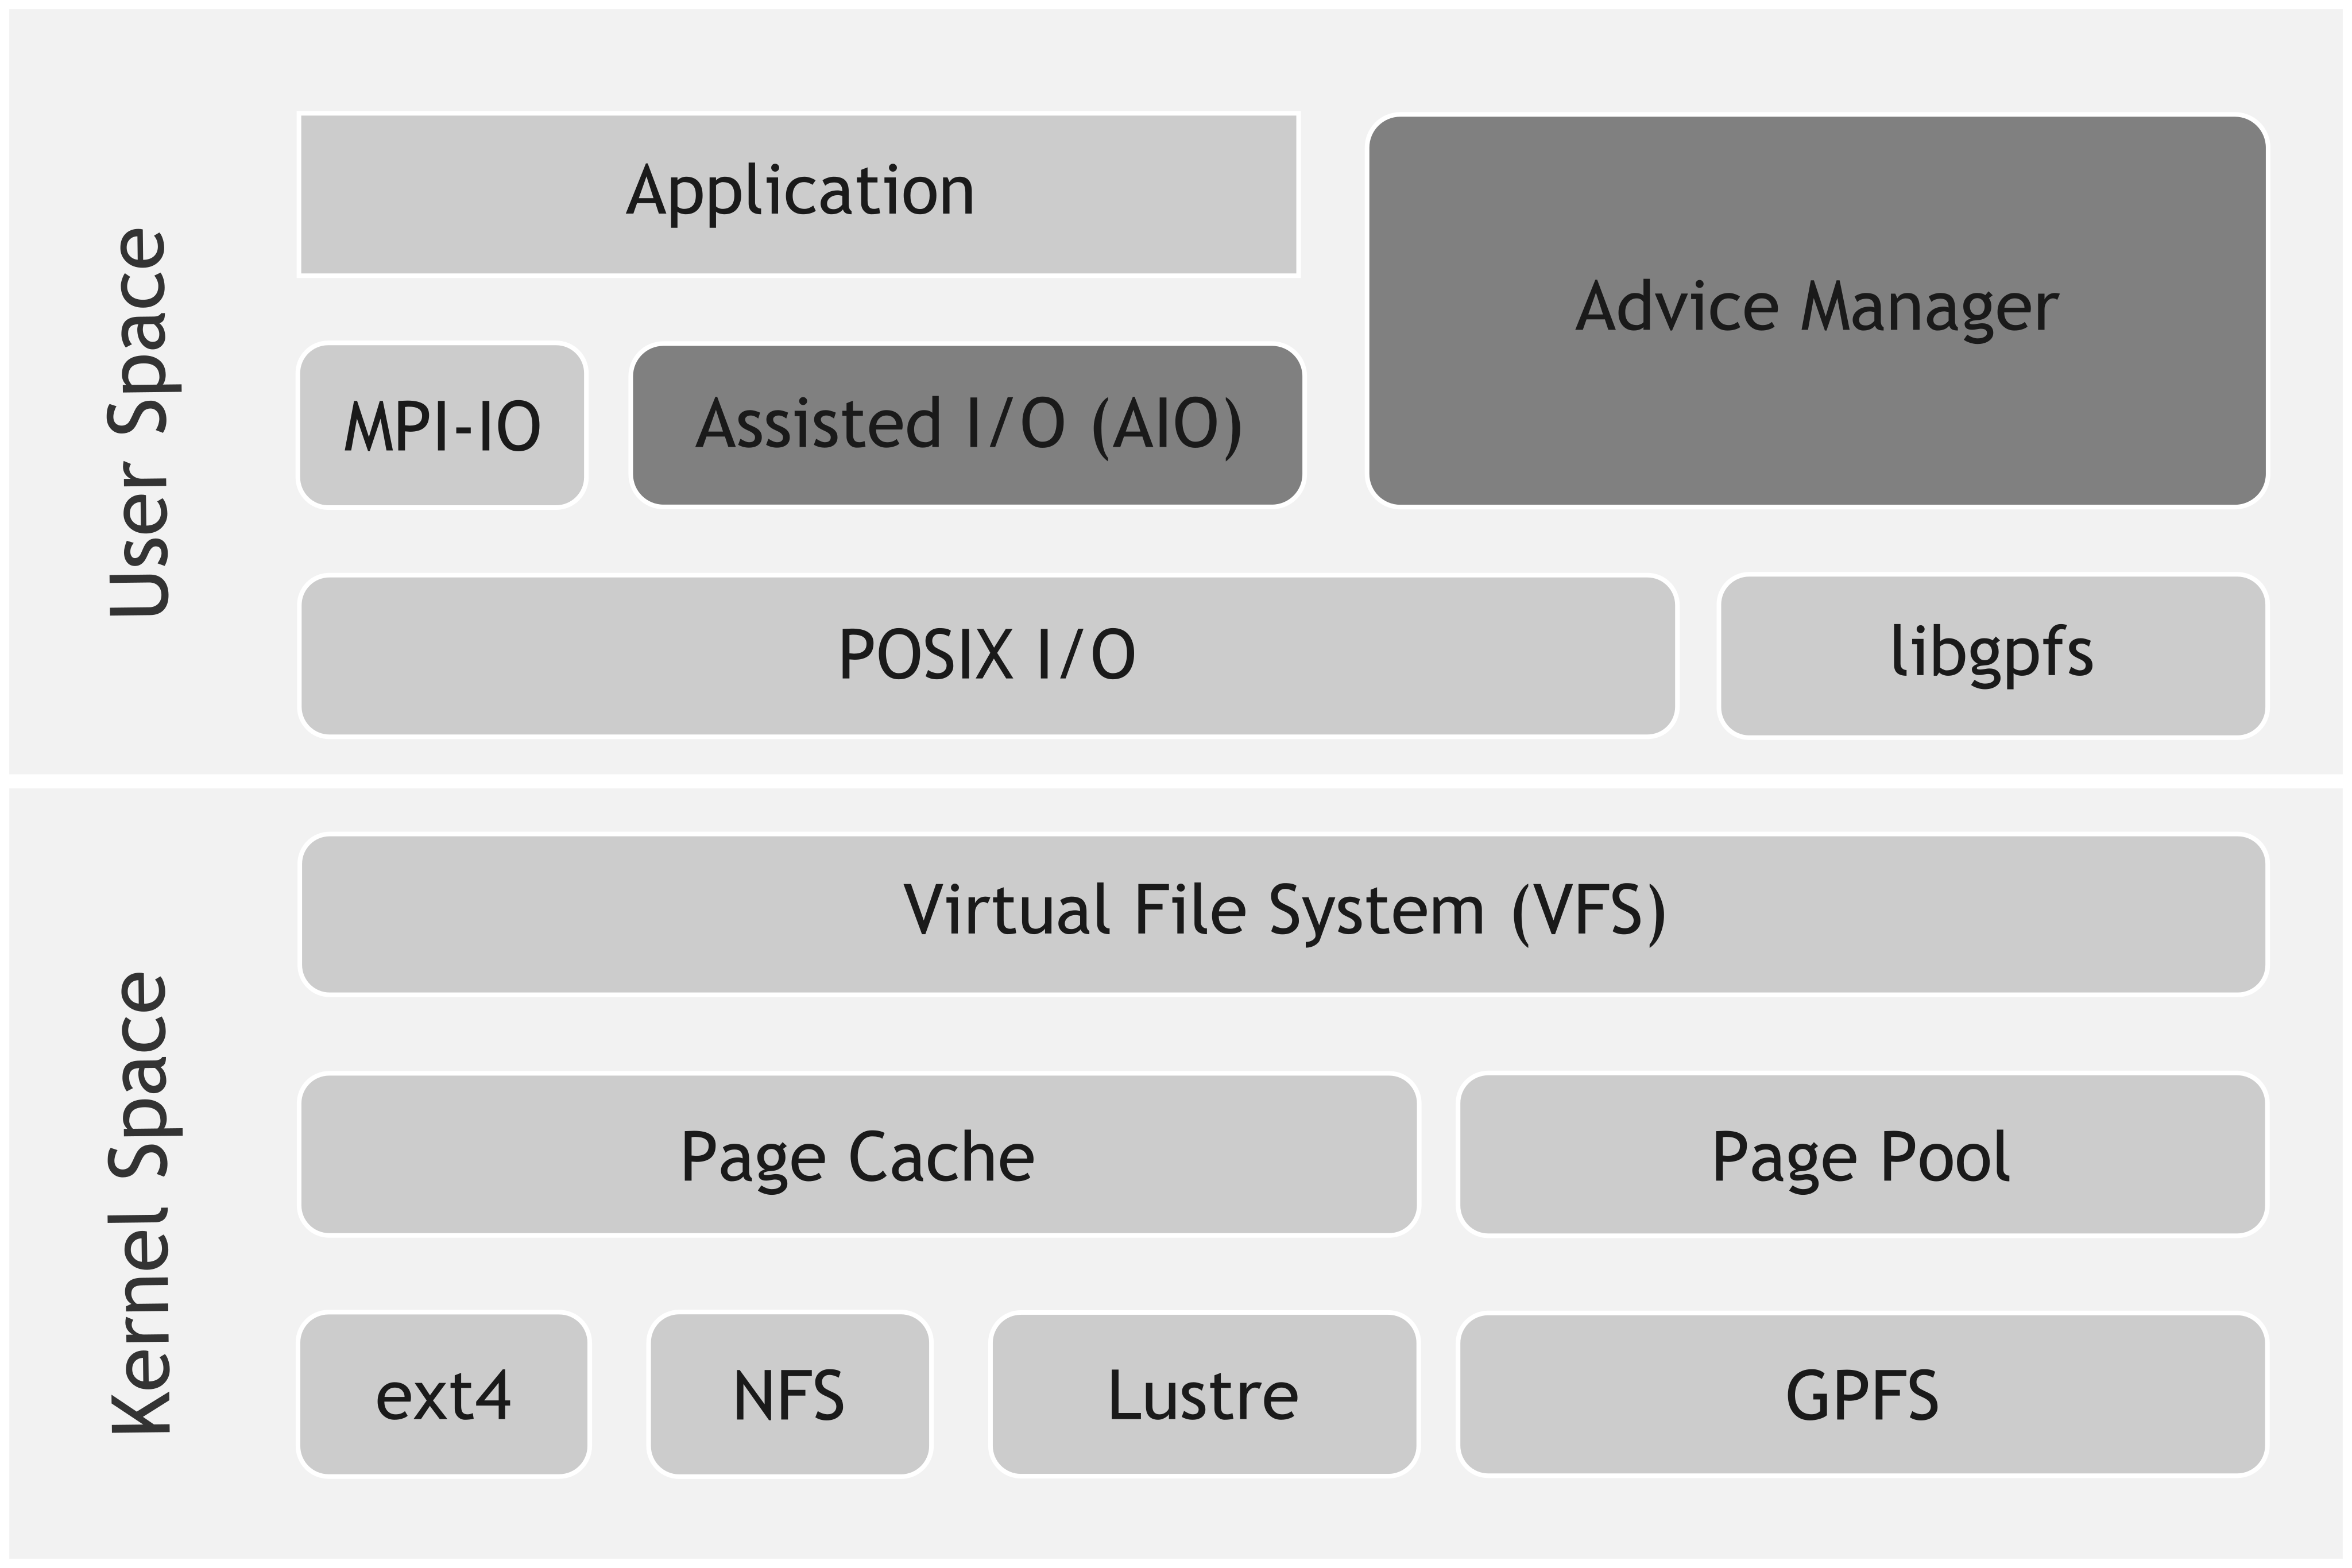
\includegraphics[width=0.8\textwidth]{figures/linux-software-stack-ext}
  \caption{Mercury I/O software stack. \textit{assisted I/O library} and \textit{advice manager} communicate through UNIX domain sockets. The AM binds its socket to the local file system pathname \texttt{/tmp/channel}, while the AIO connects its 
  socket to the same pathname; exactly in the same way they would bind and connect to an IP address if they were located on different nodes in the network. Unix domain sockets are used to pass ancillary data as well as custom messages between the 
  two software entities. Data can reside in a local Linux file system, in Lustre or in GPFS.}
  \label{figure: softwarestack}
\end{figure}

The proposed architecture adds two major contributions. First of all, it allows us to use the Linux advice API as well as the GPFS hints API asynchronously through the \textit{advice manager}. This means that we can effectively overlap I/O and 
computation phases in target applications. Secondly, it enables us to generate POSIX advice and GPFS hints transparently, without the need to modify the application. The information required by the \textit{advice manager} is extracted from 
observations of the application's I/O behaviour~\footnote{How this can be done effectivelly and in a generalized way is itself a research topic and is therefore left as part of future works.} during a set of preliminary runs and then written to 
a configuration file to be used in following runs.

In the rest of this section we describe the different aspects of our design including the interprocess communication between the two software entities and the prefetching request generation using the \texttt{posix\_fadvise()} system call or the 
\texttt{gpfs\_fcntl()} function.

\subsection{Interprocess Communication}
We now describe how interprocess communication is implemented and how messages sent from the \textit{assisted I/O library} are handled by the \textit{advice manager}. Figure~\ref{figure: architecture} depicts the architecture of the two software 
components introduced by our design. The \textit{advice manager} is made up of three smaller modules: a \textit{request manager} (RM) that receives requests sent by the \textit{assisted I/O library}, a \textit{register log} (RL) that keeps track 
of which files are currently handled by the \textit{advice manager}, and an \textit{advisor thread} (AT) that receives read requests from the \textit{request manager} through a queue and issues POSIX advice and GPFS hints.

In order to enable asynchronous prefetching we delegate the task of sending synchronous hints or advice to the \textit{advice manager}. When an application issues an open call for a file, the \textit{assisted I/O library} intercepts it, performs 
the open and then sends a message to the \textit{advice manager}. The message contains a string of the form: \texttt{"\textbf{Register} \textit{pid} \textit{pathname} \textit{fd}"}, plus additional ancillary information explained later. This string 
tells the \textit{request manager} to register the pid of the process opening the file with pathname and file descriptor number, in the register log. As a consequence the \textit{request manager} performs two operations, first it asks the 
\textit{request log} to register the new file. From this point on, future read calls for the file will be monitored by the \textit{advice manager}. Second, it creates a new \textit{advisor thread} that will take care of generating POSIX advice or 
GPFS hints depending on which file system the file resides in. I/O calls coming from the application are never blocked by the \textit{assisted I/O library}. The reason is that the \textit{advice manager} can become congested by too many requests 
coming from different processes and we do not want to reflect this on the behaviour of the application.  %The register operation is described by the flow diagram shown in Figure~\ref{figure: register_operation}.

\begin{figure}[!htb]
  \centering
  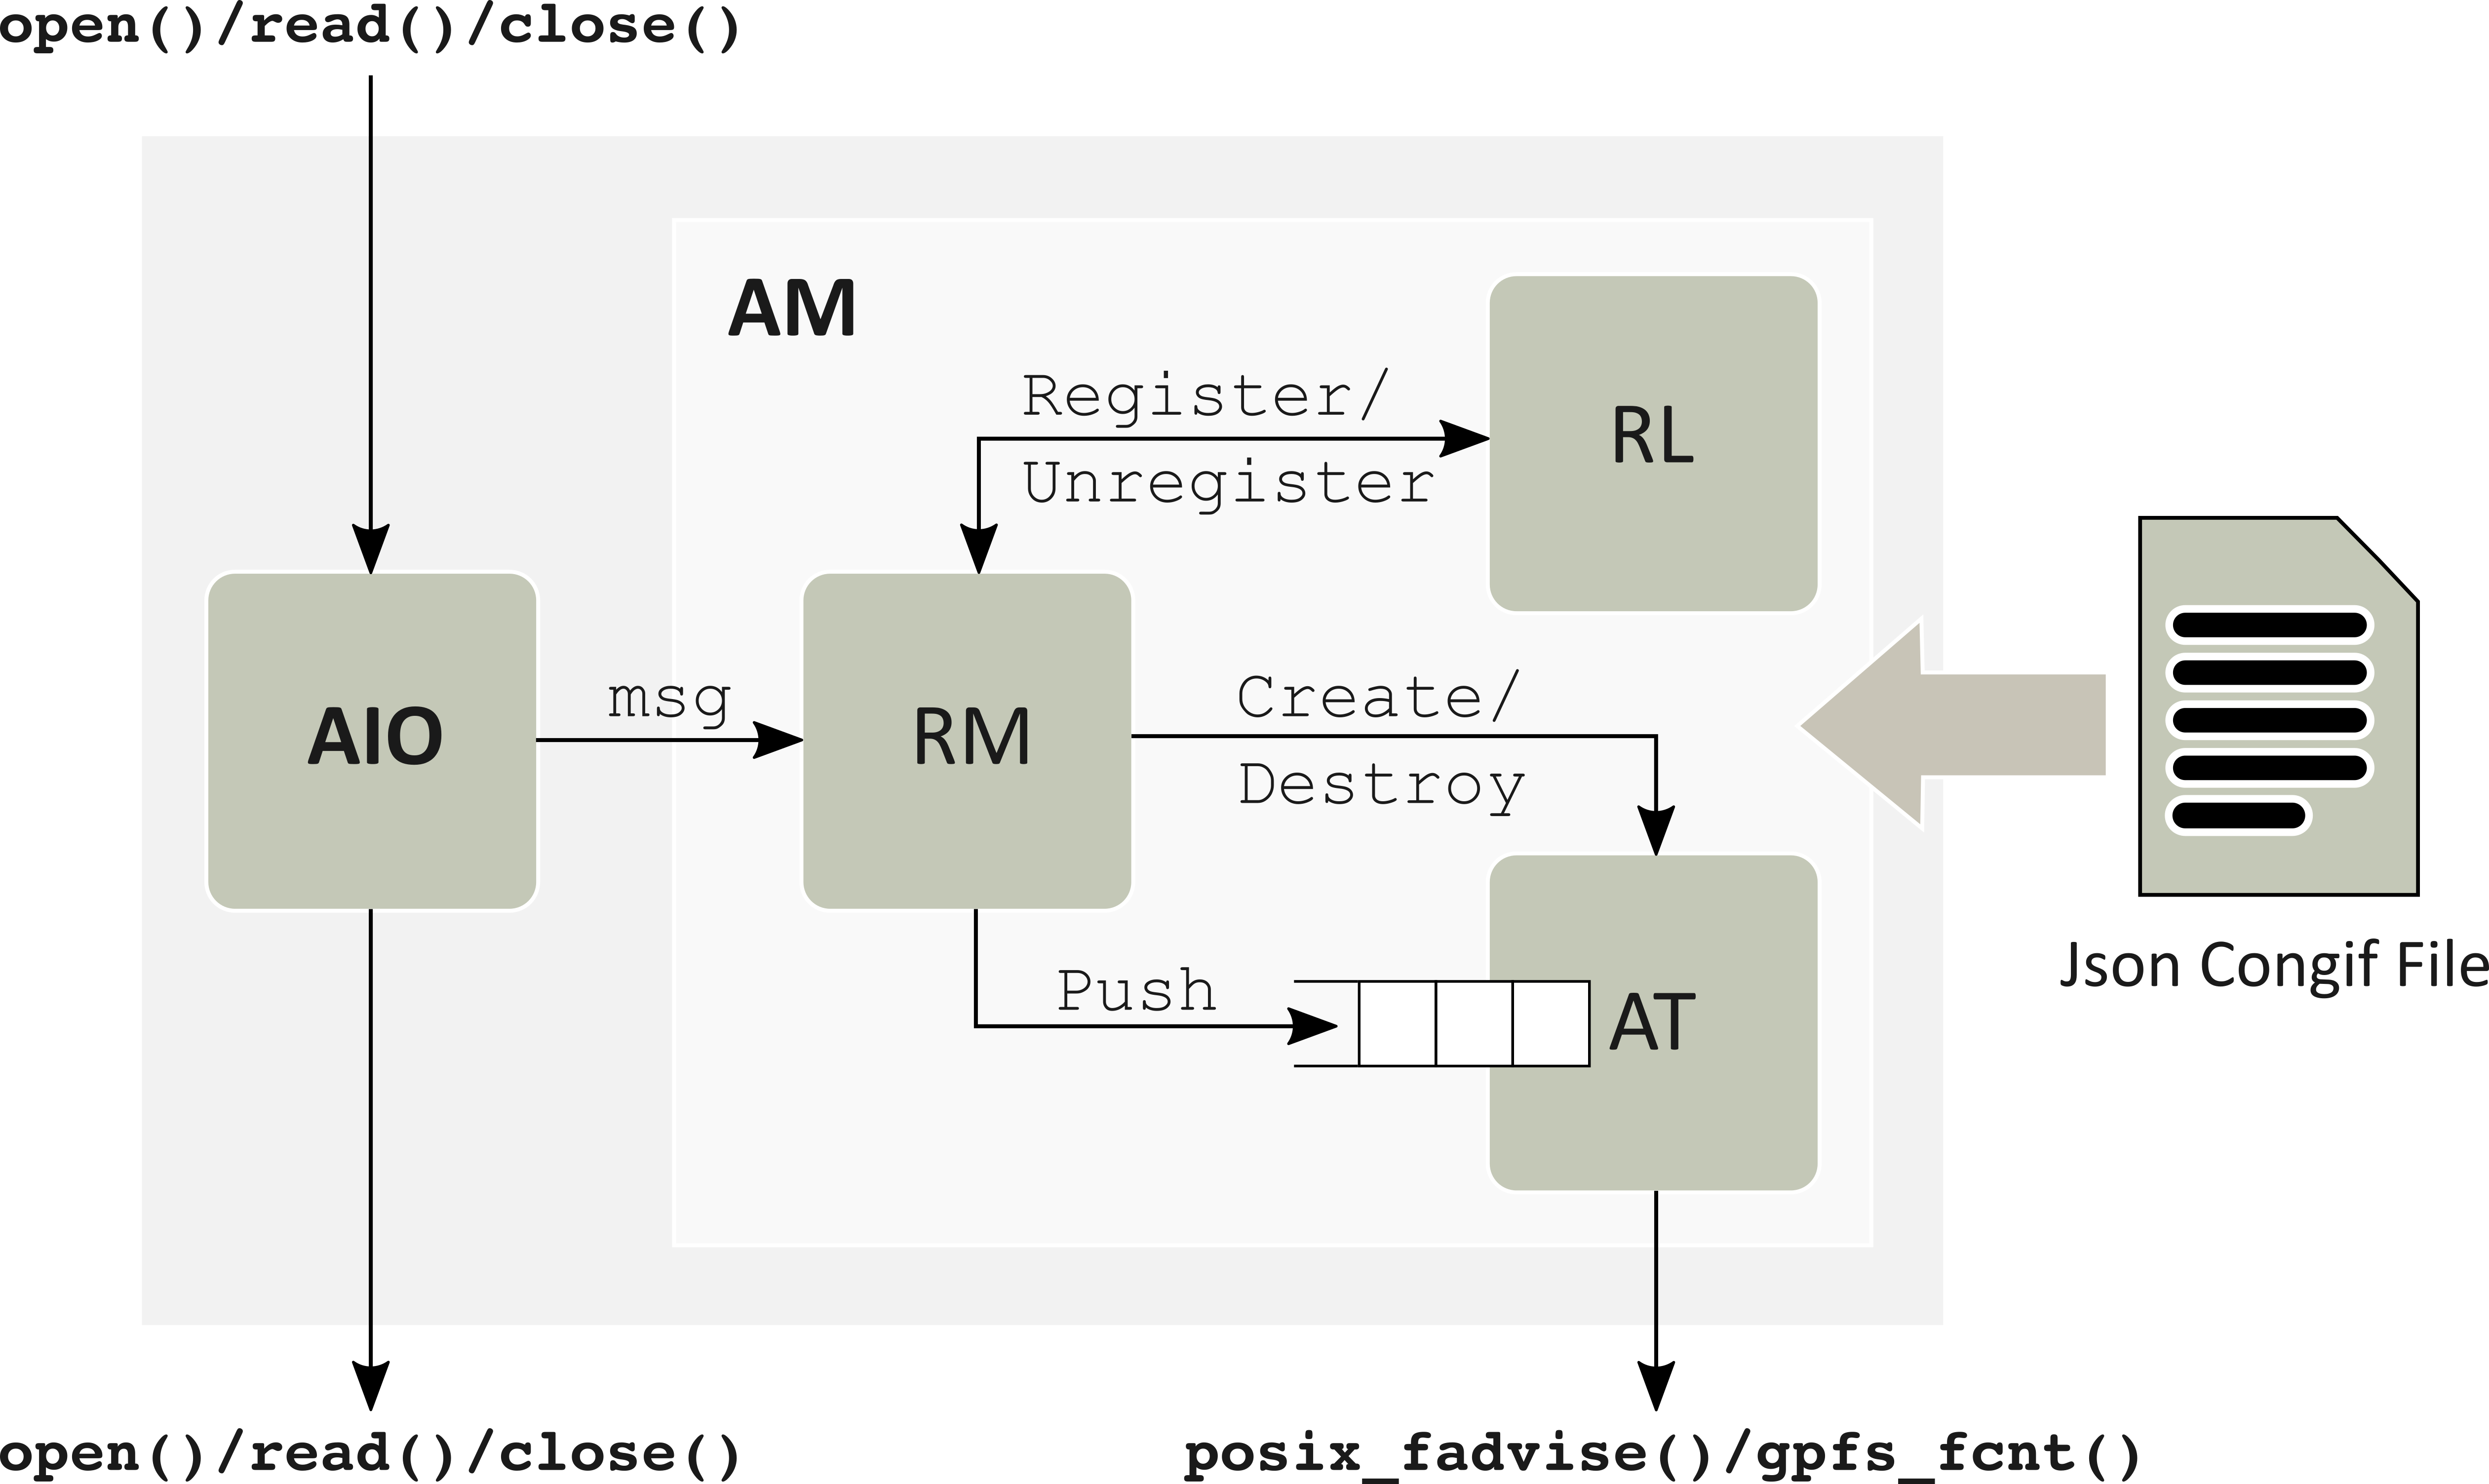
\includegraphics[width=0.8\textwidth]{figures/mercury-architecture}
  \caption{Detailed architecture for the \textit{Advice Manager} (AM) component. This can be further divided into three blocks: \textit{Request Manager} (RM), \textit{Register Log} (RL), and \textit{Advisor Thread} (AT).}
  \label{figure: architecture}
\end{figure}

Both POSIX advice and GPFS hints affect an open file, identified by its file descriptor number. For the \textit{advice manager} to send advice or hints on behalf of the application, it needs to share the open file with the application. When sending 
messages from the \textit{assisted I/O library} to the \textit{advice manager} we use \texttt{sendmsg()}. Besides normal data, this system call allows the transfer of ancillary (or control) information. One use of such information is to send a remote 
process a `file descriptor'~\cite{StevensR13} via a UNIX domain socket~\cite{UnixSock}. These numbers are just an index into the kernel's list of a process's open files. When sending a file descriptor using \texttt{sendmsg()}, the kernel copies a new 
reference to the open file descriptor, and adds it to the receiving process's open files list. The \textit{advice manager} receives a new file descriptor number, (which will likely be different to the number sent), which points to a file descriptor 
shared with the application. This allows us to send hints or advice for the shared file.

\subsection{File Data Prefetching}
POSIX advice and GPFS hints are issued using the \textit{advisor thread} created by the \textit{request manager} during the register operation (Figure~\ref{figure: architecture}). When an application performs a read operation for an open file, the 
\textit{assisted I/O library} sends to the \textit{advice manager} a message containing a string of the form: \texttt{"\textbf{Read} \textit{pid} \textit{fd} \textit{off} \textit{len}"}. This string includes the pid of the process, the application's 
file descriptor number for the file, the offset within the file and the length of the request. The pid and the file descriptor number are used by the \textit{request manager} module only to identify the corresponding \textit{advisor thread}. When the 
correct thread has been identified the \textit{request manager} pushes the offset and the length of the read request into a queue. This queue is accessed by the \textit{advisor thread} that uses the read information to trigger prefetch requests using 
the local file descriptor and keeps track of all the prefetched data using a block cache data structure. %Figure~\ref{figure: read_operation} shows the flow diagram for the read operation. 

The \textit{advisor thread} uses \texttt{posix\_fadvise()} and \texttt{gpfs\_fcntl()} to generate prefetch requests for the underlying file systems (Figure~\ref{figure: architecture}). For files residing in local file systems and Lustre, the 
\texttt{POSIX\_FADV\_WILLNEED} advice from Table~\ref{table: advice_table} is used to bring the data into the kernel page cache. For files residing in GPFS the \texttt{accRangeArray} in the \texttt{gpfsMultipleAccessRange\_t} data structure in 
Listing~\ref{mar} is used to define which blocks of the file should be brought into the GPFS internal cache (page pool). 
The size of the file regions to prefetch is defined inside a Json\footnote{Open standard format that uses human-readable text to transmit data objects consisting of attribute-value pairs (\url{http://www.rfc-editor.org/rfc/rfc7159.txt}).} configuration file, 
loaded at startup by both the \textit{advice manager} and the \textit{assisted I/O library}. This is the only point of configuration for the user and it contains, besides other information, a list of files and directories that the \textit{assisted I/O library} 
should monitor. An example configuration file is shown below. 

\begin{lstlisting}[language=python, caption=Example of Json Configuration File, label={config}]
{
    "File": {
        "Path": "/path/to/target/file",
        "BlockSize": 4194304,
        "CacheSize": 8,
        "ReadAheadSize": 4,
        "WillNeed": {
            "Offset": 0,
            "Length": 0
        }
    },
    "Directory": {
        "Path": "/path/to/target/dir",
        "Random": {
            "Offset": 0,
            "Length": 0
        }
    }
}
\end{lstlisting}

As it can be seen in Listing~\ref{config} the structure of the configuration file is very simple. It allows users to define which files POSIX advice or GPFS hints should be applied to by setting the \texttt{Path} field to the full file path and the regions of 
the file that are likely to be accessed in terms of offset and length. In the case of POSIX advice users can also define directories to which a global advice should be applied (e.g., randomly accessed files in the directory). Additionally, when indicating 
a \texttt{WillNeed} advice users can directly control the caching behaviour of the \textit{advisor thread} block cache. In particular, they can define the granularity of the prefetch request (\texttt{BlockSize}), how many blocks can be fitted into the \textit{advisor thread} 
cache (\texttt{CacheSize}) and how many blocks of data should be read ahead starting from the current accessed block (\texttt{ReadAheadSize}). Clearly the example in Listing~\ref{config} is not exhaustive. More complex configuration files can be generated by administrators 
(or automatic tools) to dynamically change the I/O patterns of applications in order to best adapt them to the underlying storage system.

The replacement policy for the block cache in the \textit{advisor thread} uses an LRU algorithm. In order to prefetch data, the open file is divided into blocks of size `BlockSize' and entire blocks are loaded/released into/from memory as the application 
progresses. In the case of GPFS the \texttt{accRangeArray} hint is used to prefetch up to `ReadAheadSize' blocks ahead starting from the block touched by the current request. When the number of blocks in the cache has reached `CacheSize', if more blocks are 
requested, older blocks will be released using the \texttt{relRangeArray} hint to make space for the new ones. In the case of POSIX advice, the behaviour is the same but blocks are loaded into memory using the \texttt{POSIX\_FADV\_WILLNEED} advice and released 
using the \texttt{POSIX\_FADV\_DONTNEED} advice. The hints interface is automatically selected by the \textit{advice manager} at runtime depending on the file system hosting the target file. 

The \textit{advisor thread} block cache also provides a very basic level of coordination among processes accessing the same file. In fact, different \textit{advisor thread} instances hinting the same file on behalf of different processes share the same block 
cache. Blocks requested by one process will appear in the block cache and future accesses to those blocks by other processes will not trigger new prefetching requests.

In general the configuration file can be used to describe any of the advice listed in Table~\ref{table: advice_table} and the hints listed in Table~\ref{table: hints_table}. To define a new scenario, we may consider a file region accessed sequentially for which 
the \texttt{POSIX\_FADV\_SEQUENTIAL} advice type could be used, and another region accessed randomly for which the \texttt{POSIX\_FADV\_RANDOM} advice type could be used. In this case, the configuration file would contain a list of file regions, specifying which 
type of advice messages are suitable. The right advice will be selected according to which part of the file is being accessed currently. This feature allows us to overcome another limitation of the Linux advice implementation that has been mentioned in 
Section~\ref{section: hints_interface}, namely, the first three advice types apply to the whole file since the implementation in the kernel completely disregards the byte ranges specified by the user.
 
Finally, when the application closes the file the \textit{assisted I/O library} sends to the \textit{advice manager} a message containing a string of the form: \texttt{"\textbf{Unregister} \textit{pid} \textit{fd}"}. This string includes the pid of the process 
and the file descriptor number of the file to be closed. In response to this request the \textit{request manager} tells the \textit{register log} to unregister the file and destroys the \textit{advisor thread}, it also closes its shared copy of the file.

\subsection{POSIX Advice integration with Lustre}
Lustre is a high performance parallel file system for Linux clusters. It works in kernel space and takes advantage of the available page cache infrastructure. Additionally, it extends POSIX read and write operations with distributed locks to provide data 
consistency across the whole cluster. Even though Lustre makes use of the Linux kernel page cache, the previously described POSIX advice syscall has no effect on Lustre. The reason can be understood by looking at Figure~\ref{figure: kernel}. This reports 
the simplified call graph for the Lustre read operation in the file system client. To simplify the explanation, the figure is divided into four quadrants. Along the x-axis we have the native kernel functions (e.g., \texttt{generic\_file\_aio\_read}), separated 
by the Lustre specific functions (e.g., \texttt{lustre\_generic\_file\_read}). Along the y-axis we have page operations (e.g., \texttt{find\_get\_page}) separated by the file operations (e.g., \texttt{generic\_file\_aio\_read}). 

We can notice that Lustre extends the kernel code with additional file and page operations through the Lustre Lite component. These are the functions used by the kernel to fill the file operations table and the address space operations table. The 
\texttt{posix\_fadvise()} system call in the kernel translates into \texttt{fadvise64()}. In the case of \texttt{POSIX\_FADV\_WILLNEED} this function directly invokes \texttt{force\_page\_cache\_readahead()} which has no effect on \texttt{ll\_readpage()}. 
Other advice such as \texttt{POSIX\_FADV\_\{NORMAL,SEQUENTIAL,RANDOM\}} are disabled in Lustre by setting the kernel readahead window size to zero. This is done so that lustre will not speculatively try to gain a highly-contended lock to fulfil an optimistic 
readahead request.

\begin{figure}[!htb]
  \centering
  \includegraphics[width=\textwidth]{figures/linux_lustre}
  \caption{Simplified function call graph for the read operation in Lustre. For page operations in the Linux kernel the picture also shows the call graph typically followed by local reads as well as the call graph for the 
  \texttt{POSIX\_FADV\_WILLNEED} advice in the \texttt{posix\_fadvise()} implementation (dashed line).}
  \label{figure: kernel}
\end{figure}

In order to enable \texttt{POSIX\_FADV\_WILLNEED} in Lustre we modified the call graph of \texttt{fadvise64()} presented in Figure~\ref{figure: kernel} to invoke the \texttt{aio\_read()} operation in the file operations table for the open file and block 
until all the data has been read into the page cache. In this way we can force the kernel to invoke the corresponding file read operation in Lustre, acquiring locks as appropriate. Of course this mechanism still works with local file systems which eventually 
will end up calling \texttt{force\_page\_cache\_readahead()} as in the original version.

To prevent the new generated read from altering the readahead state of normal read operations, in \texttt{fadvise64()} we create a new \texttt{struct file} using the \texttt{dentry\_open()} routine and set the access mode flag (\texttt{f\_mode}) of the 
new file to \texttt{FMODE\_RANDOM} (which is exactly what the \texttt{POSIX\_FADV\_RANDOM} advice message does to disable readahead for random accessed files). This mechanism works perfectly with local file systems but has no effect on Lustre's readahead 
algorithm which is independent from the Linux kernel readahead. Therefore, \texttt{POSIX\_FADV\_WILLNEED} in the case of Lustre prefetches a bit more data than requested. This is acceptable for now but a future implementation will also modify the Lustre 
code to make sure the behaviour is the same in both cases.

Finally, our kernel patch does not require any user buffer to be provided with the new read operation. To avoid data being copied to user space we pass a null pointer to the \texttt{aio\_read()} routine. Additionally we defined a new \texttt{ki\_flag} 
for the kernel I/O control block (\texttt{kiocb}), that we called \texttt{KIF\_FORCE\_READ\_AHEAD}. This new flag is checked in the \texttt{generic\_file\_aio\_read()} routine and if set the \texttt{do\_generic\_file\_read()} routine is invoked with a 
pointer to the \texttt{file\_read\_actor\_dummy()} routine. \texttt{file\_read\_actor()} is normally the routine responsible for copying the data from the page cache to the user space buffer. Since in our case there is no user space buffer, the dummy 
routine just returns success.

\section{Contributions} \label{section: mercury_related_work}
In the past researchers have tried to alleviate the I/O gap by analyzing I/O patterns and exploiting their knowledge to guide I/O using, for example, data prefetching. Tran and Reed~\cite{TranR04} presented an automatic 
time series modelling and prediction framework for adaptive I/O prefetching, named TsModeler. They combined ARIMA and Markov models to describe temporal and spatial behaviour of I/O patterns at file block level. TsModeler 
was integrated with the experimental file system PPFS2 to predict future accesses and tested against a selected physics code. Several characteristics, such as execution time improvements and cache miss reduction over different 
hardware configurations, are considered in the experiments. The results show that execution time can be reduced by the 30\% in some cases and cache misses can be reduced up to three order of magnitude. 

He et al.~\cite{HeBTAGGMCS13} proposed a pattern detection algorithm, based on the sliding window algorithm in LZ77 as base for building Markov models of I/O patterns at file block level. The model was afterwards used by a FUSE 
based file system to carry out prefetching. Chang and Gibson~\cite{ChangG99}, unlike previous works, did not build mathematical models but instead used speculative execution of the application code to guide data prefetching. Some 
authors have also used code analysis during source code compilation to automatically insert prefetch hints and hide disk latency to applications~\cite{Mowry1996}~\cite{Brown2000}~\cite{Brown2001}.

Other works tried to bring the same idea to higher level I/O libraries such as MPI-IO, HDF5 or PnetCDF to take advantage of the richer semantic, data dependencies and layout information. Chen et al.~\cite{ChenBSTG08} proposed a 
pre-execution based prefetching approach to mask I/O latency. They provided every MPI process with a thread that runs in parallel and takes responsibility for prefetching future required data. Prefetching in the parallel thread 
was enabled via speculative execution of the main process code. Results, with PBench running on top of NFS and PVFS as file systems backend, show execution time reduction and sustained bandwidth improvements. The same authors in
~\cite{Byna2008} proposed to exploit parallel prefetching using a client-side, thread based, collective prefetching cache layer for MPI-IO. The cache layer used I/O pattern information, in the form of I/O signatures, together 
with run-time I/O information to predict future accesses. Experimental results show sustained bandwidth improvements even in this case. 

Chen and Roth~\cite{ChenR10} took inspiration from the collective I/O optimization enabled by ROMIO to design a collective I/O data prefetching mechanism that exploited global I/O knowledge. They compare the sustained bandwidth 
speed-up of individual prefetching with collective prefetching for a parallel benchmarking tool using PVFS2, and demonstrate that the latter performs better than the former by over two fold on average. He et al.~\cite{HEST12} 
proposed to analyze high level data dependencies exposed in PnetCDF, accumulate this knowledge building data dependency graphs and finally use them to perform prefetching.

VanDeBogart, Frost and Kohler have previously used the Linux advice API to build a prefetching library~\cite{VanDeBogartFK09} for programmers to use. Prost et al. integrated the GPFS hint functionalities in the ROMIO ADIO driver 
for GPFS~\cite{ProstTHJK01}. In this context they exploit data type semantic in file views to prefetch parts of the file that will be soon accessed. 

In contrast to previous works, we do the following things differently. We do not try to automatically build mathematical models of I/O patterns and use them to accurately generate prefetching requests nor do we speculatively execute the application 
binary. In fact, we believe that users and administrators have the best understanding about the applications and their systems, and can exploit their knowledge and expertise to improve the storage system performance. We demonstrate that experienced 
users with a deep knowledge of their applications I/O behavior can convert non-optimal I/O patterns, in particular small random reads, into patterns that can be adapted to the underlying file system characteristics, and therefore give optimal 
performance. Furthermore, previously described approaches are not suitable for small random read patterns since they rely on accurate knowledge of I/O behaviour to prefetch every single request one after the other. This still degrades the storage 
system performance due to the large number of I/O requests and seek operations hitting the storage devices. On the other hand, by using the POSIX advice and GPFS hints APIs, we can prefetch the region of the file that will be accessed and filter 
random requests using the cache.

In this work we focus on providing the infrastructure that enables Linux users to access file system specific interfaces for guided I/O without modifying applications and hiding the intrinsic complexity that such interfaces introduce.

\chapter{NVM Based Write-behind Caching} \label{chapt: checkpointing}
HPC applications process large amounts of data that have to be written (read) to (from) large shared files residing in the global parallel file system. In order to make the dataset manageable, 
this is usually partitioned into smaller subsets and assigned to available cores for parallel processing. Complex datasets such as multi-dimensional arrays are logically flattened into a linear 
sequence of bytes and striped across several I/O targets for best performance. This results into the loss of the original spatial locality. Due to this characteristic, accesses to spatially contiguous 
regions translate into non-contiguous accesses to the file. Therefore, applications generating a large number of small, non-contiguous I/O requests to the parallel file system usually experience 
degradation of I/O performance. Such performance degradation is known as the small I/O problem and is related to the fact that parallel file systems provide best I/O bandwidth performance for large 
contiguous requests, while they typically provide only a fraction of the maximum available bandwidth in the opposite case~\cite{ChingCLP06}~\cite{HeSSYT11}. This is due to the large number of RPCs 
generated by the file system clients overwhelming I/O servers, the resulting high number of hard disk head movements in every I/O target (seek overhead) and, ultimately, to the restrictions imposed 
by the POSIX-IO write semantics that generates lock contention on file systems' blocks.

Having recognised the small I/O problem, collective I/O was proposed by the MPI-IO community~\cite{ThakurGL99}. Collective I/O exploits global I/O knowledge in parallel I/O to a shared file. This 
knowledge is used to build an aggregated view of the accessed region in the file and coalesce all the corresponding small non-contiguous requests into a smaller number of large contiguous accesses, 
later issued to the parallel file system. 

In this chapter we present our approach to improve collective I/O performance using non-volatile memory devices in HPC clusters' compute nodes. The fundamental observation that motivates our approach 
is that collective I/O performance is limited by the slowest aggregator. Aggragators experience different run-times mainly for two reasons: the communication pattern required to build file domains might 
differ among aggregators and the scheduling of requests in I/O servers might not happen simultaneously for all aggregators. These two factors, in conjunction with the need for global synchronization 
between following rounds of two phase I/O, represent the main cause of suboptimal performance.

The motivation for using a file system based write-behind approach in collective I/O is that at Exascale the amount of memory per core will shrink~\cite{ASCAC2010}. For this reason we need to make 
sure that main memory is dedicated to progressing in the computational tasks instead of the caching of large out-of-core arrays. Non-volatile memory devices provide an additional memory tier right 
between the DRAM and HDDs and can thus be used effectively as fast persistent buffers to mask remote file access time.

The remainder of this chapter is organized as follow: in Section~\ref{sec: ext2ph} we describe in detail the extended two phase algorithm at the base of the collective I/O implementation in ROMIO;
in Section~\ref{sec: coll_io_limit} we review the main performance bottlenecks in the extended two phase algorithm providing, whenever available, possible solutions to overcome each of them; 
in Section~\ref{sec: nvm-approach} we discuss in detail our proposed solution to address global synchronization limitations; finally, in Section~\ref{sec: nvm-related} we review the related works 
and outline the main differences with our approach.

\section{Extended Two Phase Algorithm} \label{sec: ext2ph}
We now describe in detail the ext2ph algorithm implementation in the ROMIO middleware. We pin-point where the major contributions to performance are located and on what aspect of collective I/O they
reflect. Figure~\ref{figure: coll_io_impl} shows the ext2ph algorithm flow diagram for collective write operations in aggregators; the diagram for non-aggregators is similar but does not contain write 
functions. (Collective read operations are not described since the behaviour is specular to the write case.) The diagram divides the algorithm into three main phases: an initialization phase (on the 
extreme left end side), the shuffle phase (on the extreme right end side), and the write phase (in the center).

\begin{figure}[H]
  \centering
  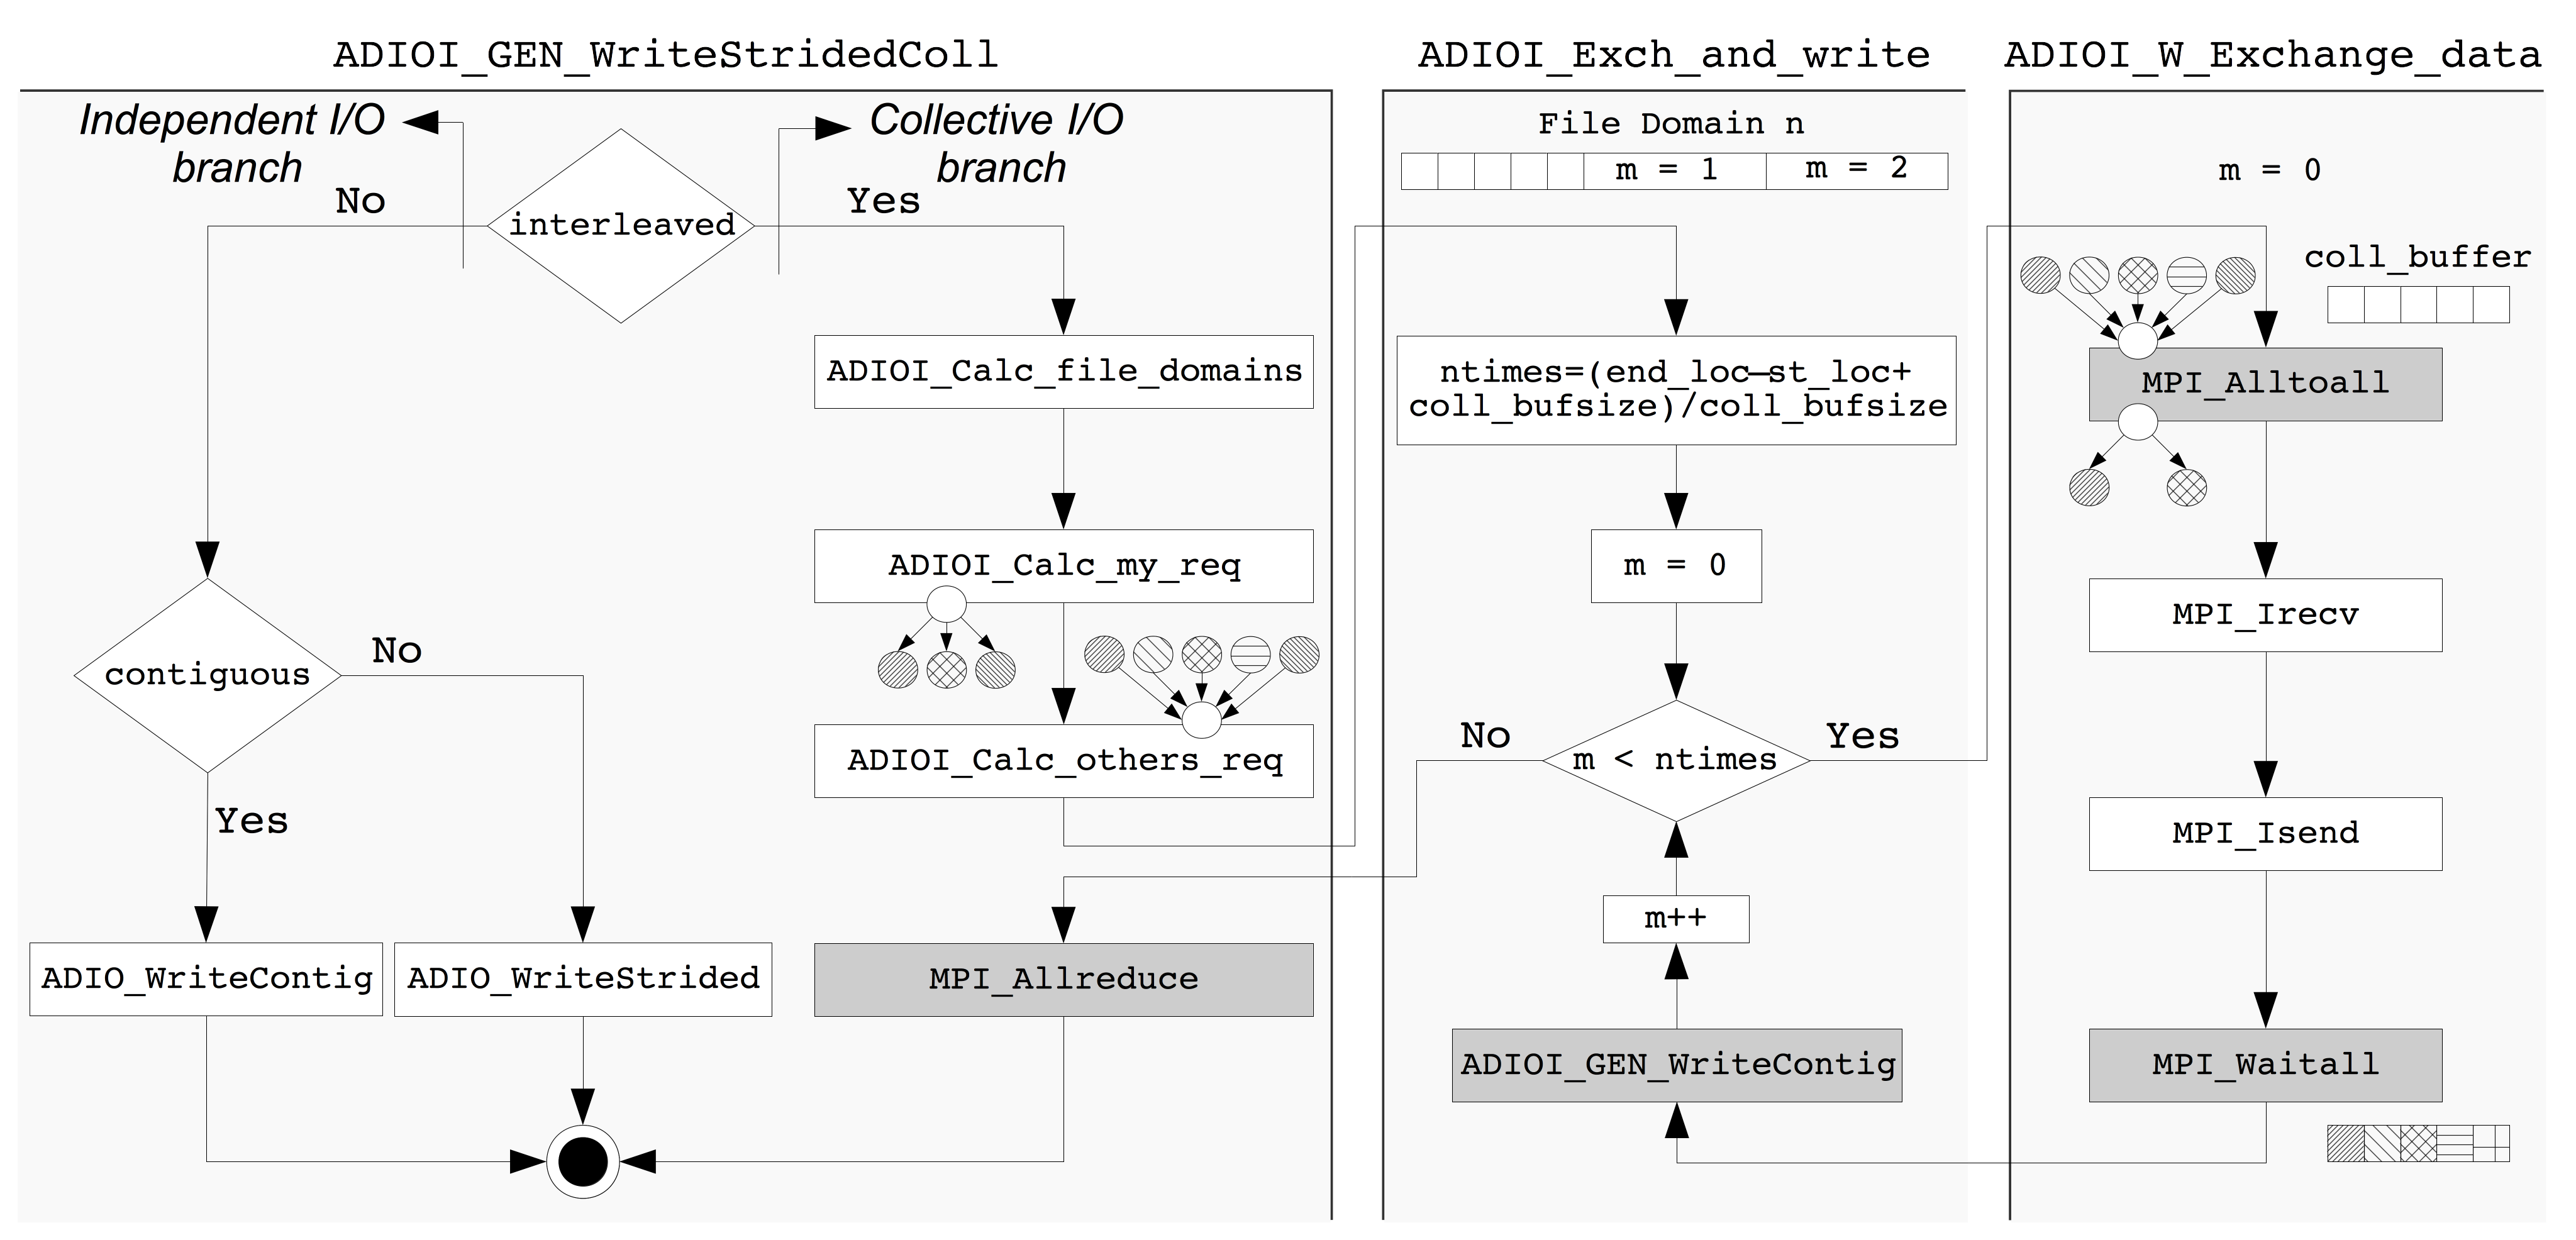
\includegraphics[angle=90, width=0.8\textwidth]{figures/ext2ph_t}
  \caption{Collective I/O flow diagram for the write path in aggregators (non-aggregators neither receive nor write any data, just send it to aggregators). \codeword{MPI\_File\_write\_all()} 
  invokes \codeword{ADIOI\_GEN\_WriteStridedColl()}. Performance critical functions for the collective I/O branch are highlighted in grey.}
  \label{figure: coll_io_impl}
\end{figure}

The \texttt{MPI\_File\_write\_all()} and \texttt{MPI\_File\_write\_at\_all()} functions are translated into the \texttt{ADIOI\_GEN\_WriteStridedColl()}\footnote{ADIOI\_LUSTRE\_WriteStridedColl() for Lustre.} 
function in the presented diagram. This function is responsible for the initialization of the ext2ph algorithm. First, it computes the file domains by dividing the aggregated access region by the number of 
available aggregators (\texttt{ADIOI\_Calc\_file\_domains}) as shown in Equation~\ref{formula: aggr-region}.

\begin{equation}\label{formula: aggr-region}
    \ceil*{\frac{MAX(end\_offset) - MIN(st\_offset)}{cb\_nodes}}
\end{equation}

Second, for every process it computes to what file domain requests belong (\texttt{ADIOI\_calc\_my\_req}) and third, for every aggregator it keeps track of what other requests fit into the file domain handled 
by the aggregator. The tracking information is stored into a \textit{file domain access table} (FDAT) and each aggregator has one to remember what parts of the file domain belong to which process in the 
application. FDATs are implemented using two arrays, one for the starting offsets and one for the lengths\footnote{A process might have more than one request for the same file domain.}. The FDATs arrays
have an entry for every process in the application, even if the process has no data in that file domain.

Once the initialization phase is complete, two phase I/O can start. Because file domains might not fit entirely in main memory, they can be broken down into smaller units using a collective buffer 
(by default this is only a few MB in size) and two phase I/O is carried out in multiple rounds of data shuffling and I/O. The central part of the diagram contains a \textit{for} loop that is iterated 
once for every round of two phase I/O. The number of rounds is computed dividing the file domain by the collective buffer size (\texttt{coll\_bufsize}).

At the beginning of the data shuffling phase (on the right end side of the diagram) every process has to communicate to aggregators what part of their file domain will be exchanged in that round. This is 
done using the \texttt{MPI\_Alltoall()} collective communication function. Afterwards, every aggregator invokes a non-blocking receive operation (\texttt{MPI\_Irecv()}) and can optionally send its own data
to other aggregators by invoking a non-blocking send operation (\texttt{MPI\_Isend()}). Finally, every aggregator waits for all the send and receive to complete by invoking \texttt{MPI\_Waitall()}. 

When the shuffling phase has completed, the collective buffer contains all the required data and it can be written to the file using \texttt{ADIOI\_GEN\_WriteContig()}. This function internally calls the standard 
POSIX-IO write operation. When all the file domains have been written to the file, aggregators need to exchange error codes to make sure that each of them has completed correctly and user buffers can be reused
for another collective write operation. This task is performed by invoking \texttt{MPI\_Allreduce()}.

There are three main performance contributions to the ext2ph implementation just described: (\textbf{a}) global synchronisation cost; (\textbf{b}) communication cost; and (\textbf{c}) write cost. \codeword{MPI\_Allreduce()} 
and \codeword{MPI\_Alltoall()} account for global synchronisation cost; when a process reaches them it has to wait for all the other processes to arrive before continuing. Because aggregators are the
only processes writing data to the parallel file system, they experience the highest run-time and the slowest aggregator among all governs the overall collective I/O performance. \codeword{MPI\_Waitall()} 
accounts for communication cost since every process first issues all the non-blocking receives (if any) and sends, and afterwards waits for them to complete. Finally, \codeword{ADIOI\_GEN\_WriteContig()} 
accounts for write cost.

The collective I/O behaviour in ROMIO can be controlled by users through a set of MPI-IO hints. Users can decide whether collective I/O should be enabled or disabled with \codeword{romio\_cb\_write} and
\codeword{romio\_cb\_read} (for write and read operations respectively), how many aggregators should be used during a collective I/O operation with \codeword{cb\_nodes} and how big the collective 
buffer should be with \codeword{cb\_buffer\_size}. Table~\ref{table: coll_io_hints_table} summarises the hints just described.

\begin{table}[!htb]
\centering
\ra{1.5}
\caption{Collective I/O hints in ROMIO.}
\newcolumntype{K}{>{\centering\arraybackslash} m{3cm}}
\newcolumntype{V}{>{\centering\arraybackslash} m{5.5cm}}
\begin{tabular}{KV}
\toprule
\bf \small Hint & \bf \small Description \\
\midrule
\small \codeword{romio\_cb\_write} & \small \codeword{enable} or \codeword{disable} collective writes \\
\small \codeword{romio\_cb\_read} & \small \codeword{enable} or \codeword{disable} collective reads \\
\small \codeword{cb\_buffer\_size} & \small set the collective buffer size [bytes]\\
\small \codeword{cb\_nodes} & \small set the number of aggregator processes\\
\bottomrule
\end{tabular}
\label{table: coll_io_hints_table}
\end{table}

Each of these hints has an effect on collective I/O performance. For example, by increasing the number of aggregators there will be a higher number of nodes writing to the parallel file 
system and thus a higher chance that one of these will experience variable performance due to different scheduling time at I/O servers, with increasing write time variation and associated 
global synchronisation cost. Furthermore, by increasing the collective buffer size users can reduce the number of two phase I/O rounds and, consequently, the number of global synchronisation 
events. Bigger collective buffers also affect the write cost since more I/O servers will be accessed in parallel potentially increasing the aggregated I/O bandwidth.

Besides the hints described in Table~\ref{table: coll_io_hints_table}, there are other hints that do not directly concern collective I/O but affect its performance. The first is the 
\codeword{striping\_factor} hint, which defines how many I/O targets (servers) will be used to store the file. The second is the \codeword{striping\_unit} hint, which defines how big the data chunks 
written to each I/O target will be (in bytes). These two hints change the file characteristics in the parallel file system and typically the striping unit also defines the block size and thus the locking 
granularity for the file (e.g., Lustre).

\section{Collective I/O Limitations} \label{sec: coll_io_limit}
%In Chapter~\ref{chapt: background} we have described in detail the extended two phase algorithm at the base of the collective I/O implementation in ROMIO. We recall that 
The goal of the extended two phase algorithm is to produce an intermediate I/O pattern in which the aggregated access region, in the logical file representation, is divided into multiple contiguous ranges, 
named \textit{file domains}, that are transfered concurrently and in liaison by aggregators to the file system. Additional interprocess communication is traded against reduced I/O cost, since this typically 
dominates performance. In this section we discuss the limitations in the ext2ph algorithm and provide for each of them possible solutions that have been explored in previous research works.

\subsection{File System Stripe Contention}
POSIX compliant file systems use locking to enforce data consistency in the file. Parallel file systems typically adopt an extent based locking strategy in which the client accessing the file
is granted a lock covering a larger portion than requested. Because the process might access other parts of the file in subsequent I/O operations, this strategy reduces the communication between 
the client and the lock manager. The way the extent based locking strategy is implemented differers between file systems. GPFS for example, uses a distributed token based approach in which the 
client requesting access to a region of the file is granted a token covering the whole file. This client becomes the owner of the lock and other clients wishing to access the file have to contact 
it in order to get tokens for other regions of the file. Lustre, on the other hand, uses a centralized server based approach in which a lock for all the file stripes, managed by a specific server,
is granted to the client. The locking mechanisms just described are presented in Figure~\ref{figure: gpfs-lock} and Figure~\ref{figure: lustre-lock} for GPFS and Lustre respectively.

\begin{figure}[!htb]
  \centering
  \begin{subfigure}[t]{0.6\textwidth}
  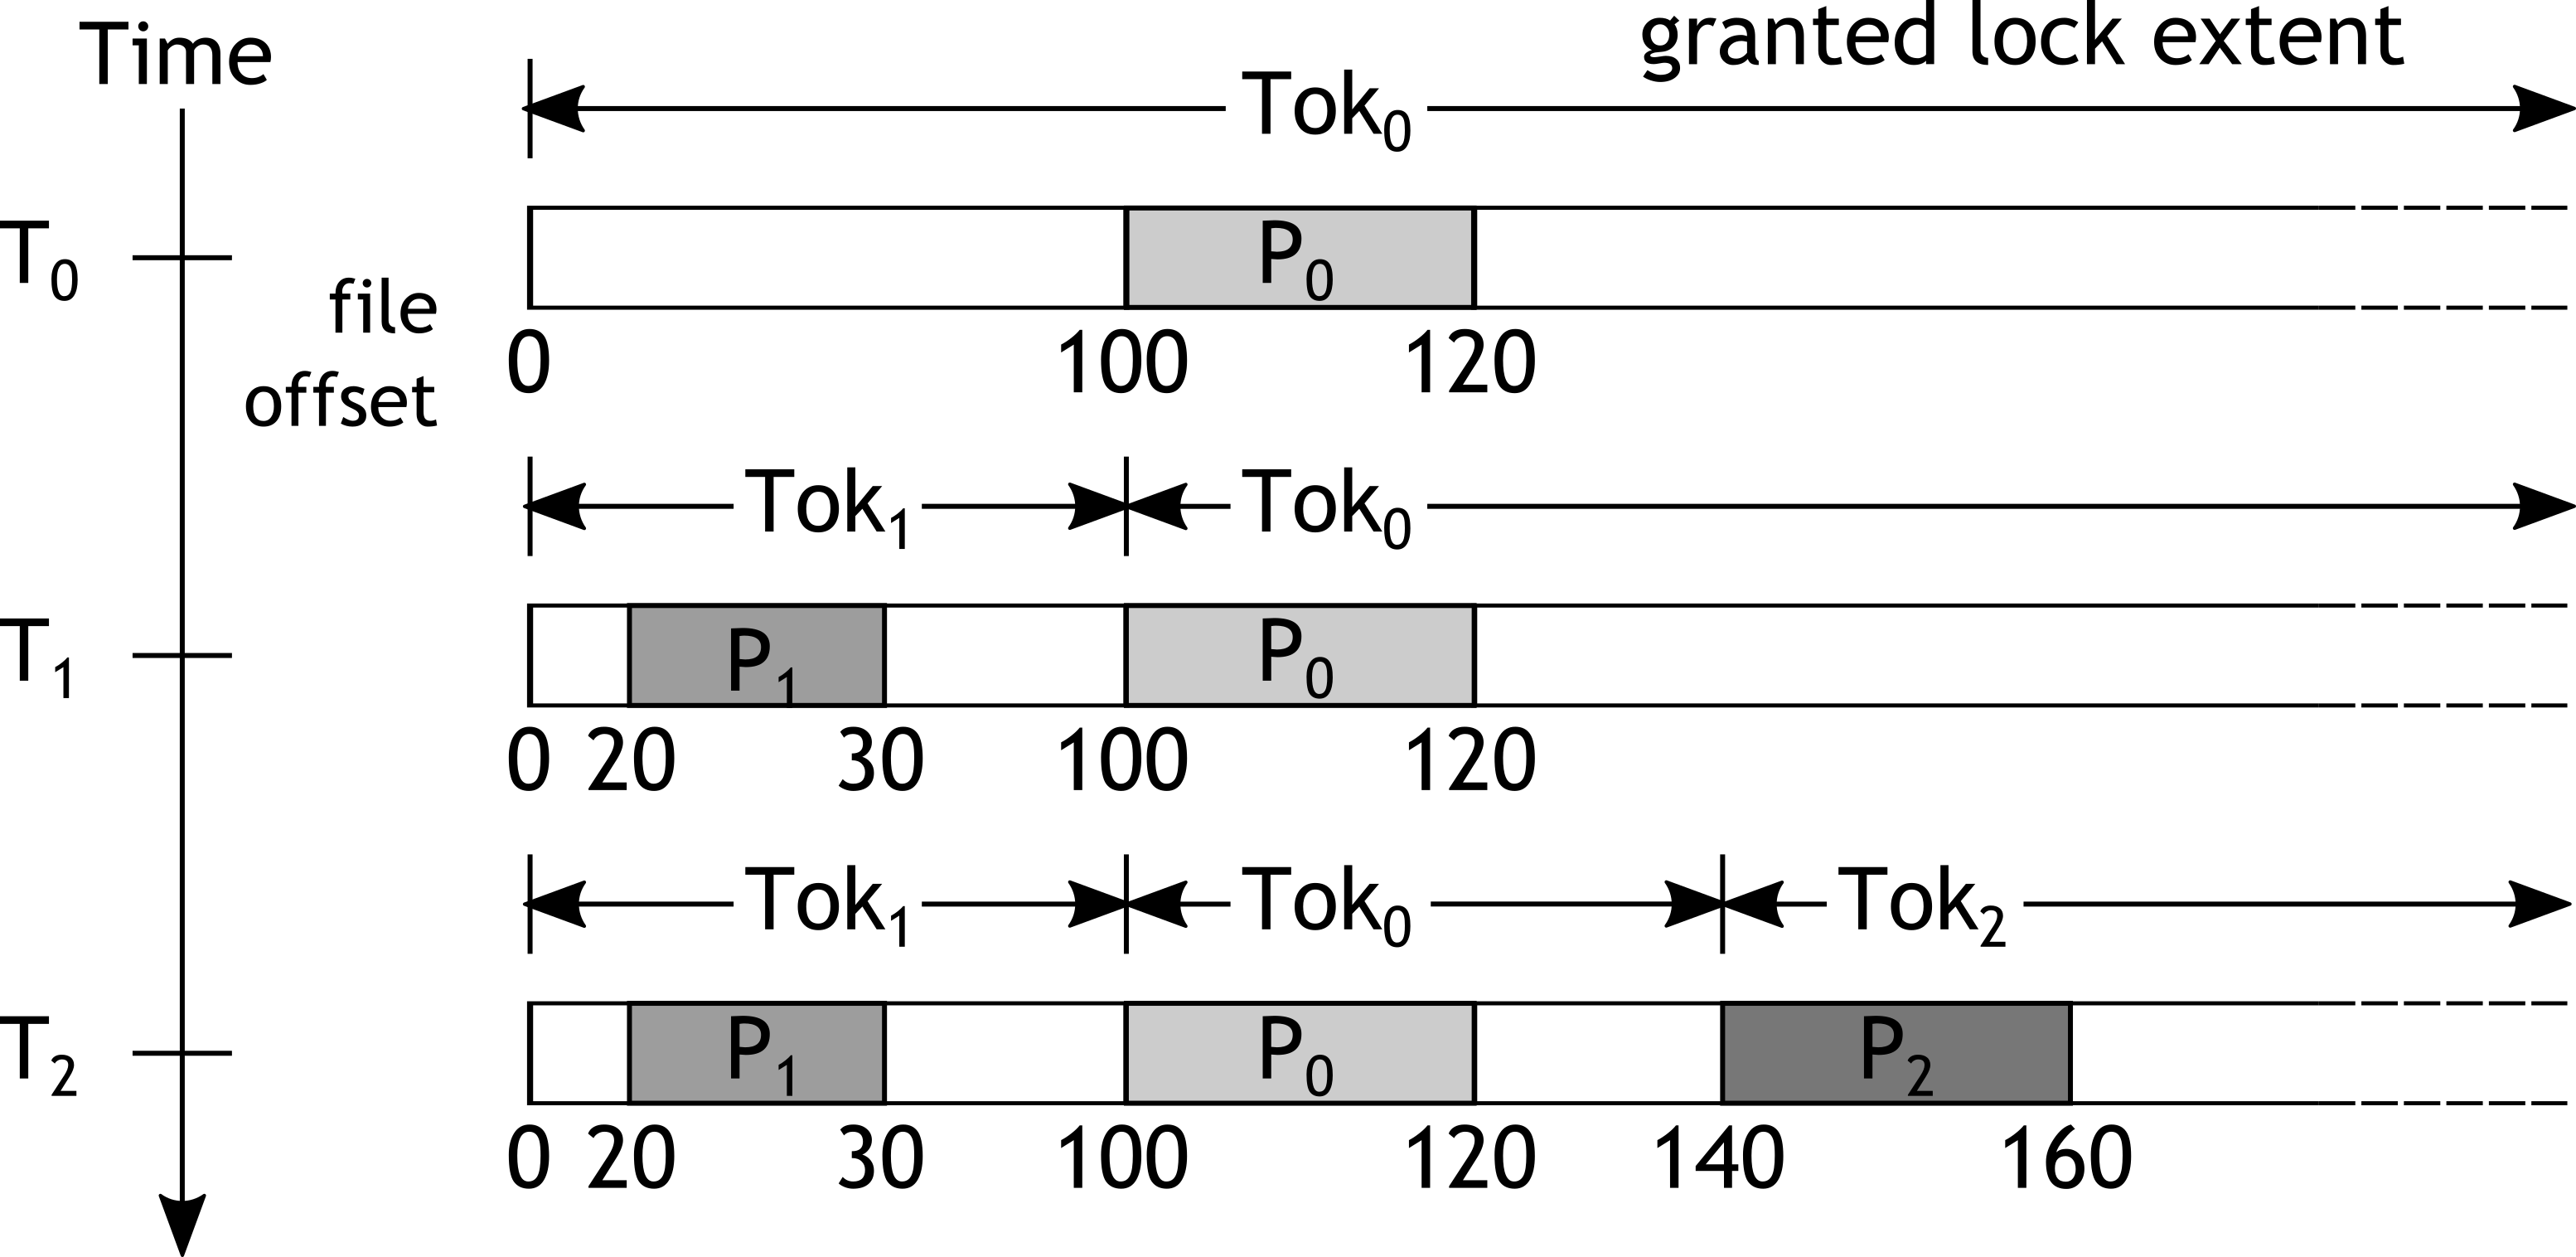
\includegraphics[width=\textwidth]{figures/gpfs-lock}
  \caption{}
  \label{figure: gpfs-lock}
  \end{subfigure}
  \begin{subfigure}[t]{0.6\textwidth}
  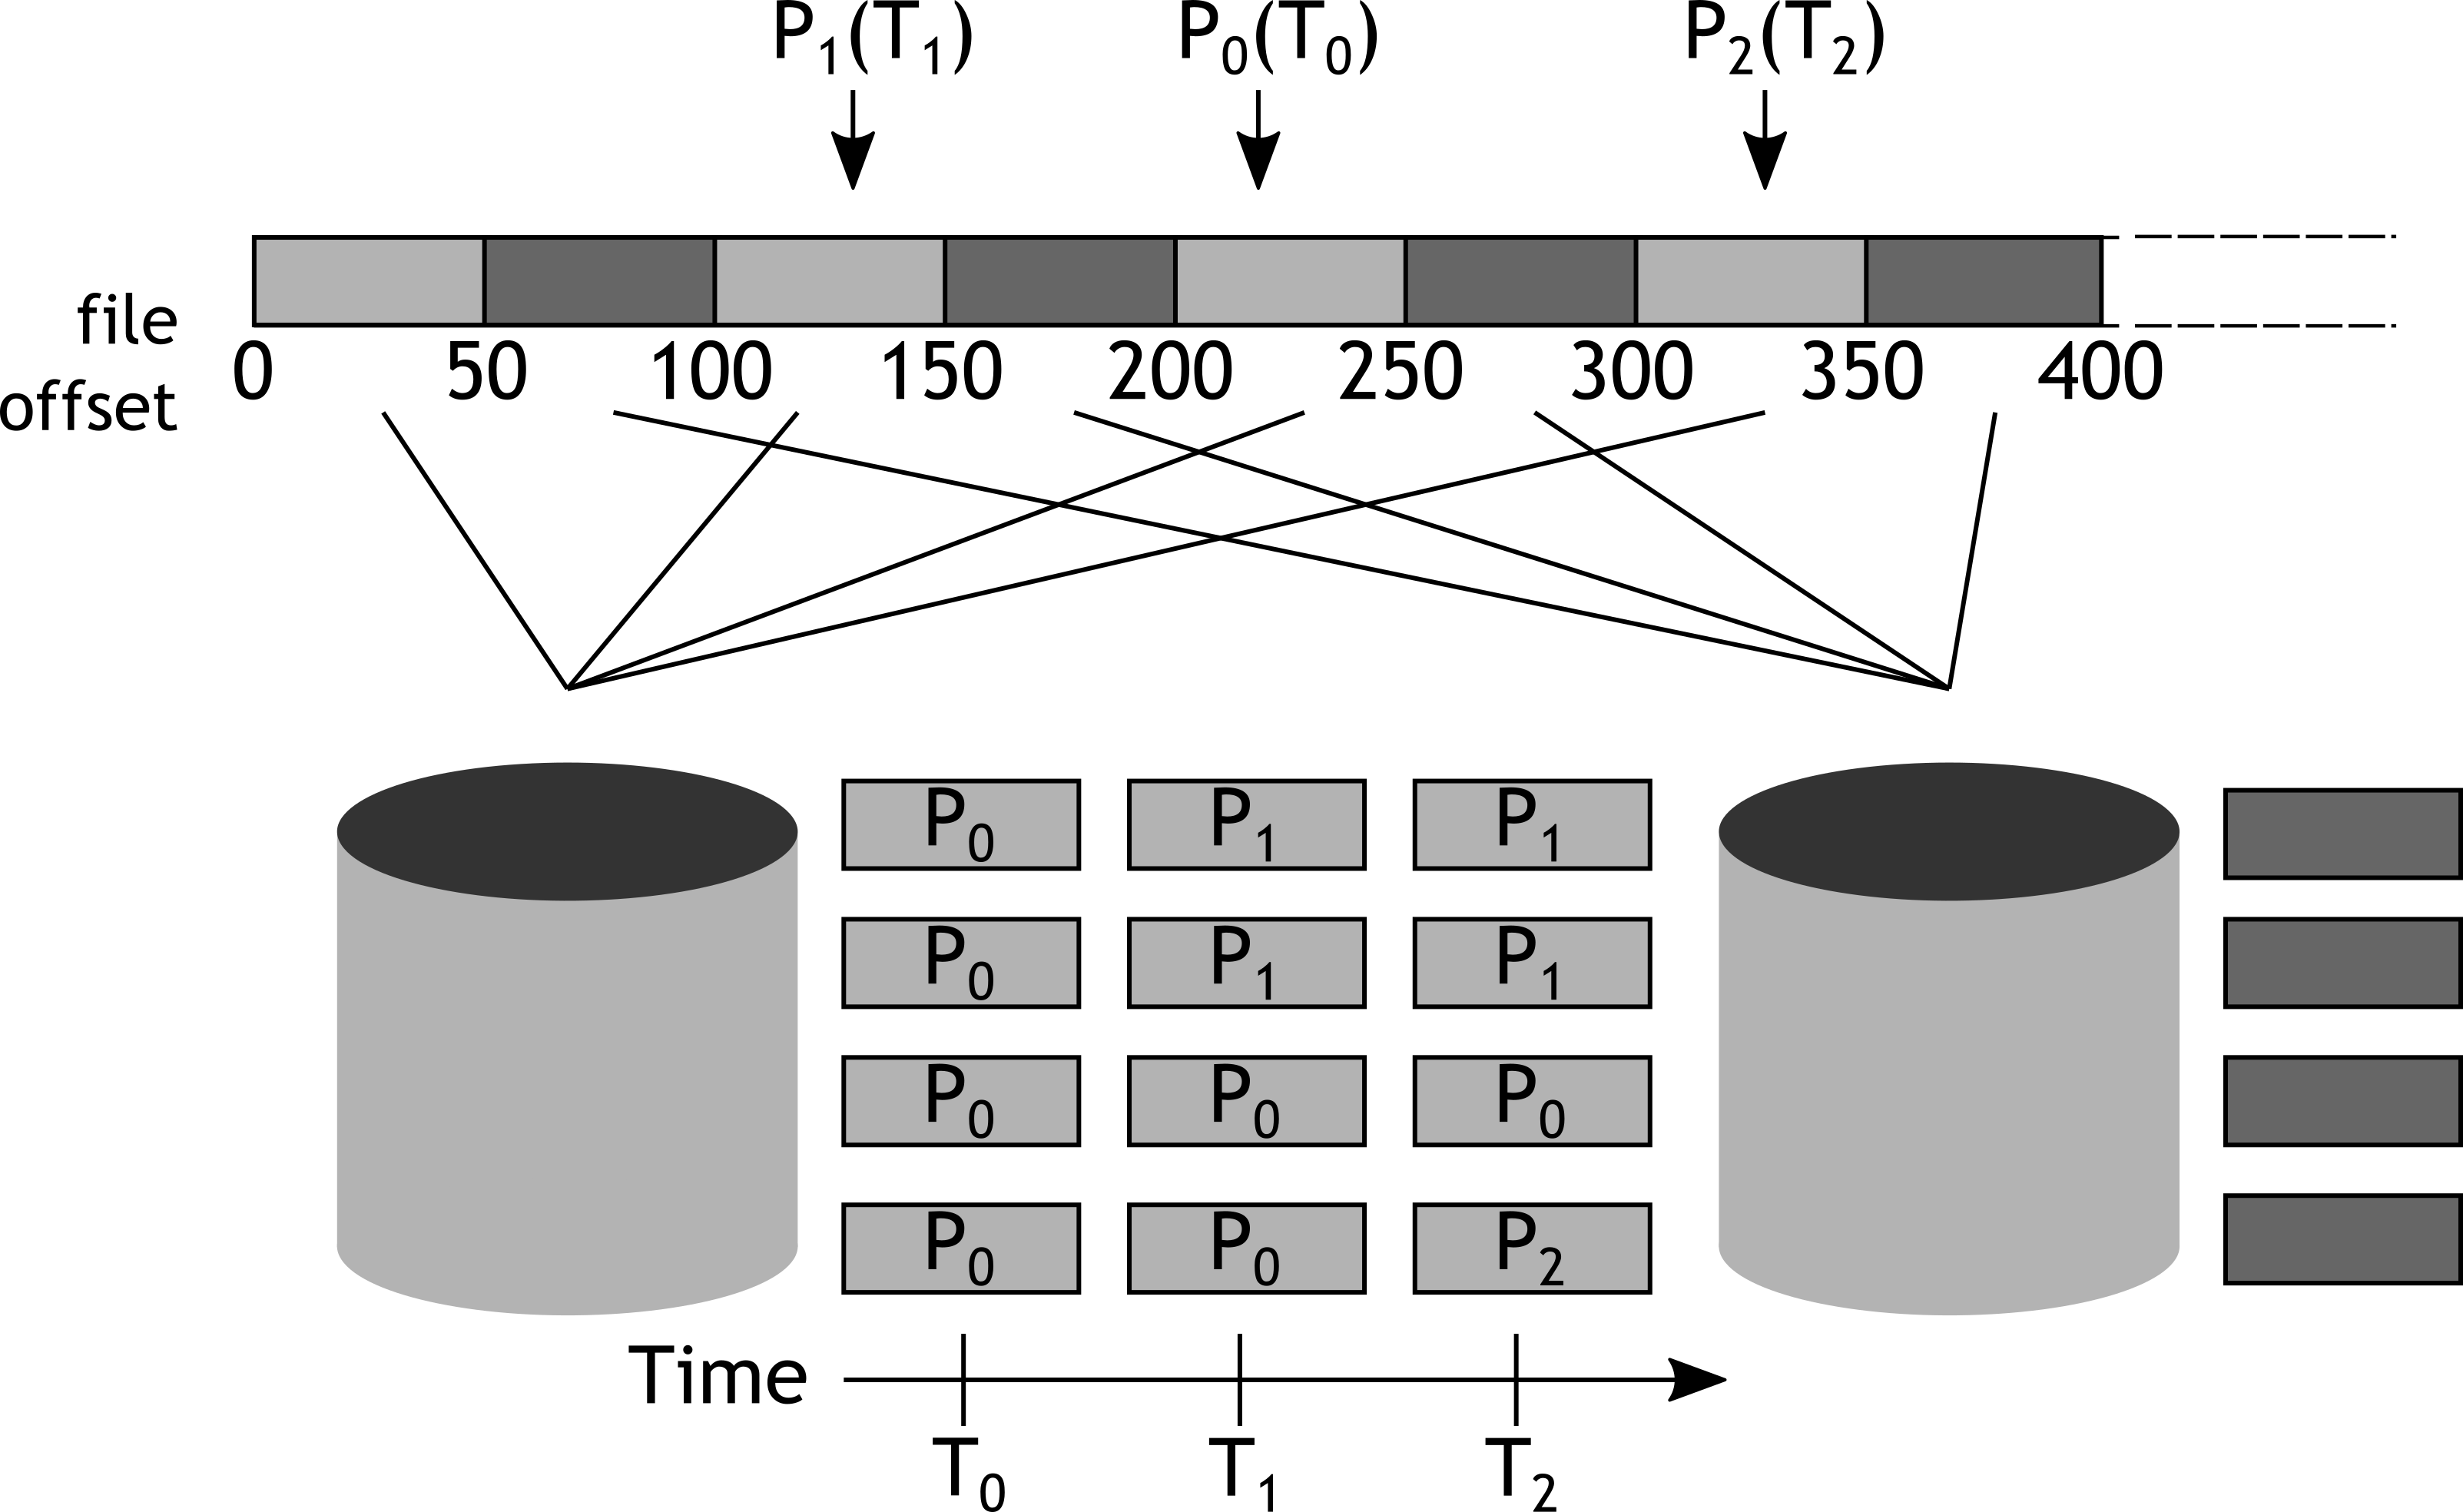
\includegraphics[width=\textwidth]{figures/lustre-lock}
  \caption{}
  \label{figure: lustre-lock}
  \end{subfigure}
  \caption{Extent based locking for GPFS~\ref{figure: gpfs-lock} and Lustre~\ref{figure: lustre-lock}. In both figures there are three process requesting access to different parts of the file
  at different times.}
\end{figure}

In the ext2ph algorithm file domains are built using an even partitioning by default. The even partitioning guarantees an optimal load balancing because every aggregator gets exactly the same
amount of data. Nevertheless, it also allows file systems stripes to be shared among multiple clients, causing false sharing of file system blocks and serializing requests at the file system level.
For this reason, it is important to make sure that file domains are built keeping the file system's locking protocol in mind. A simple solution to the problem of file system stripe contention is to
align file domains to stripe boundaries as shown in Figure~\ref{figure: gpfs-partition}.

\begin{figure}[!htb]
  \centering
  \begin{subfigure}[t]{0.8\textwidth}
  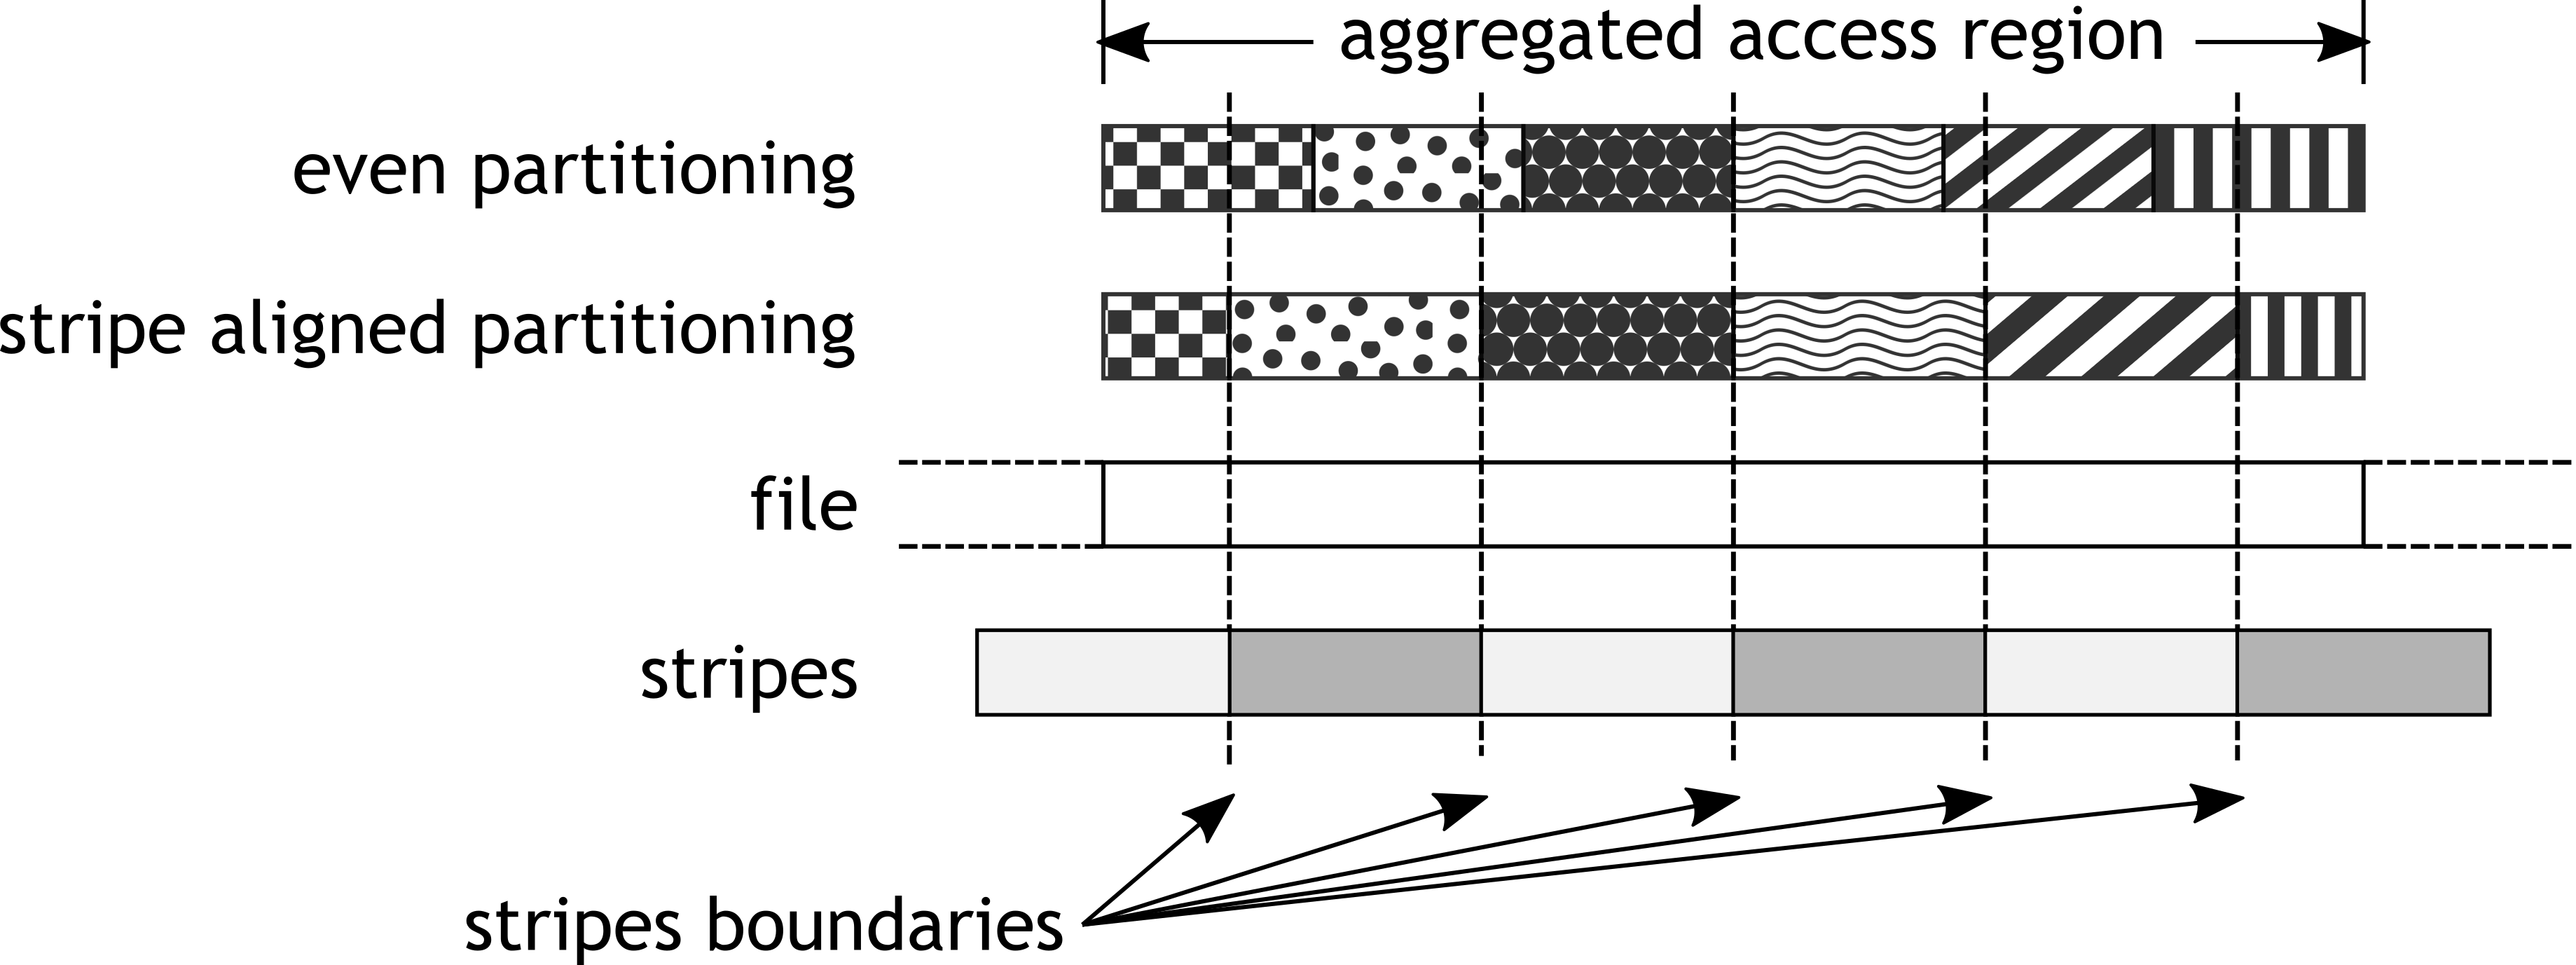
\includegraphics[width=\textwidth]{figures/gpfs-partition}
  \caption{}
  \label{figure: gpfs-partition}
  \end{subfigure}
  \begin{subfigure}[t]{0.9\textwidth}
  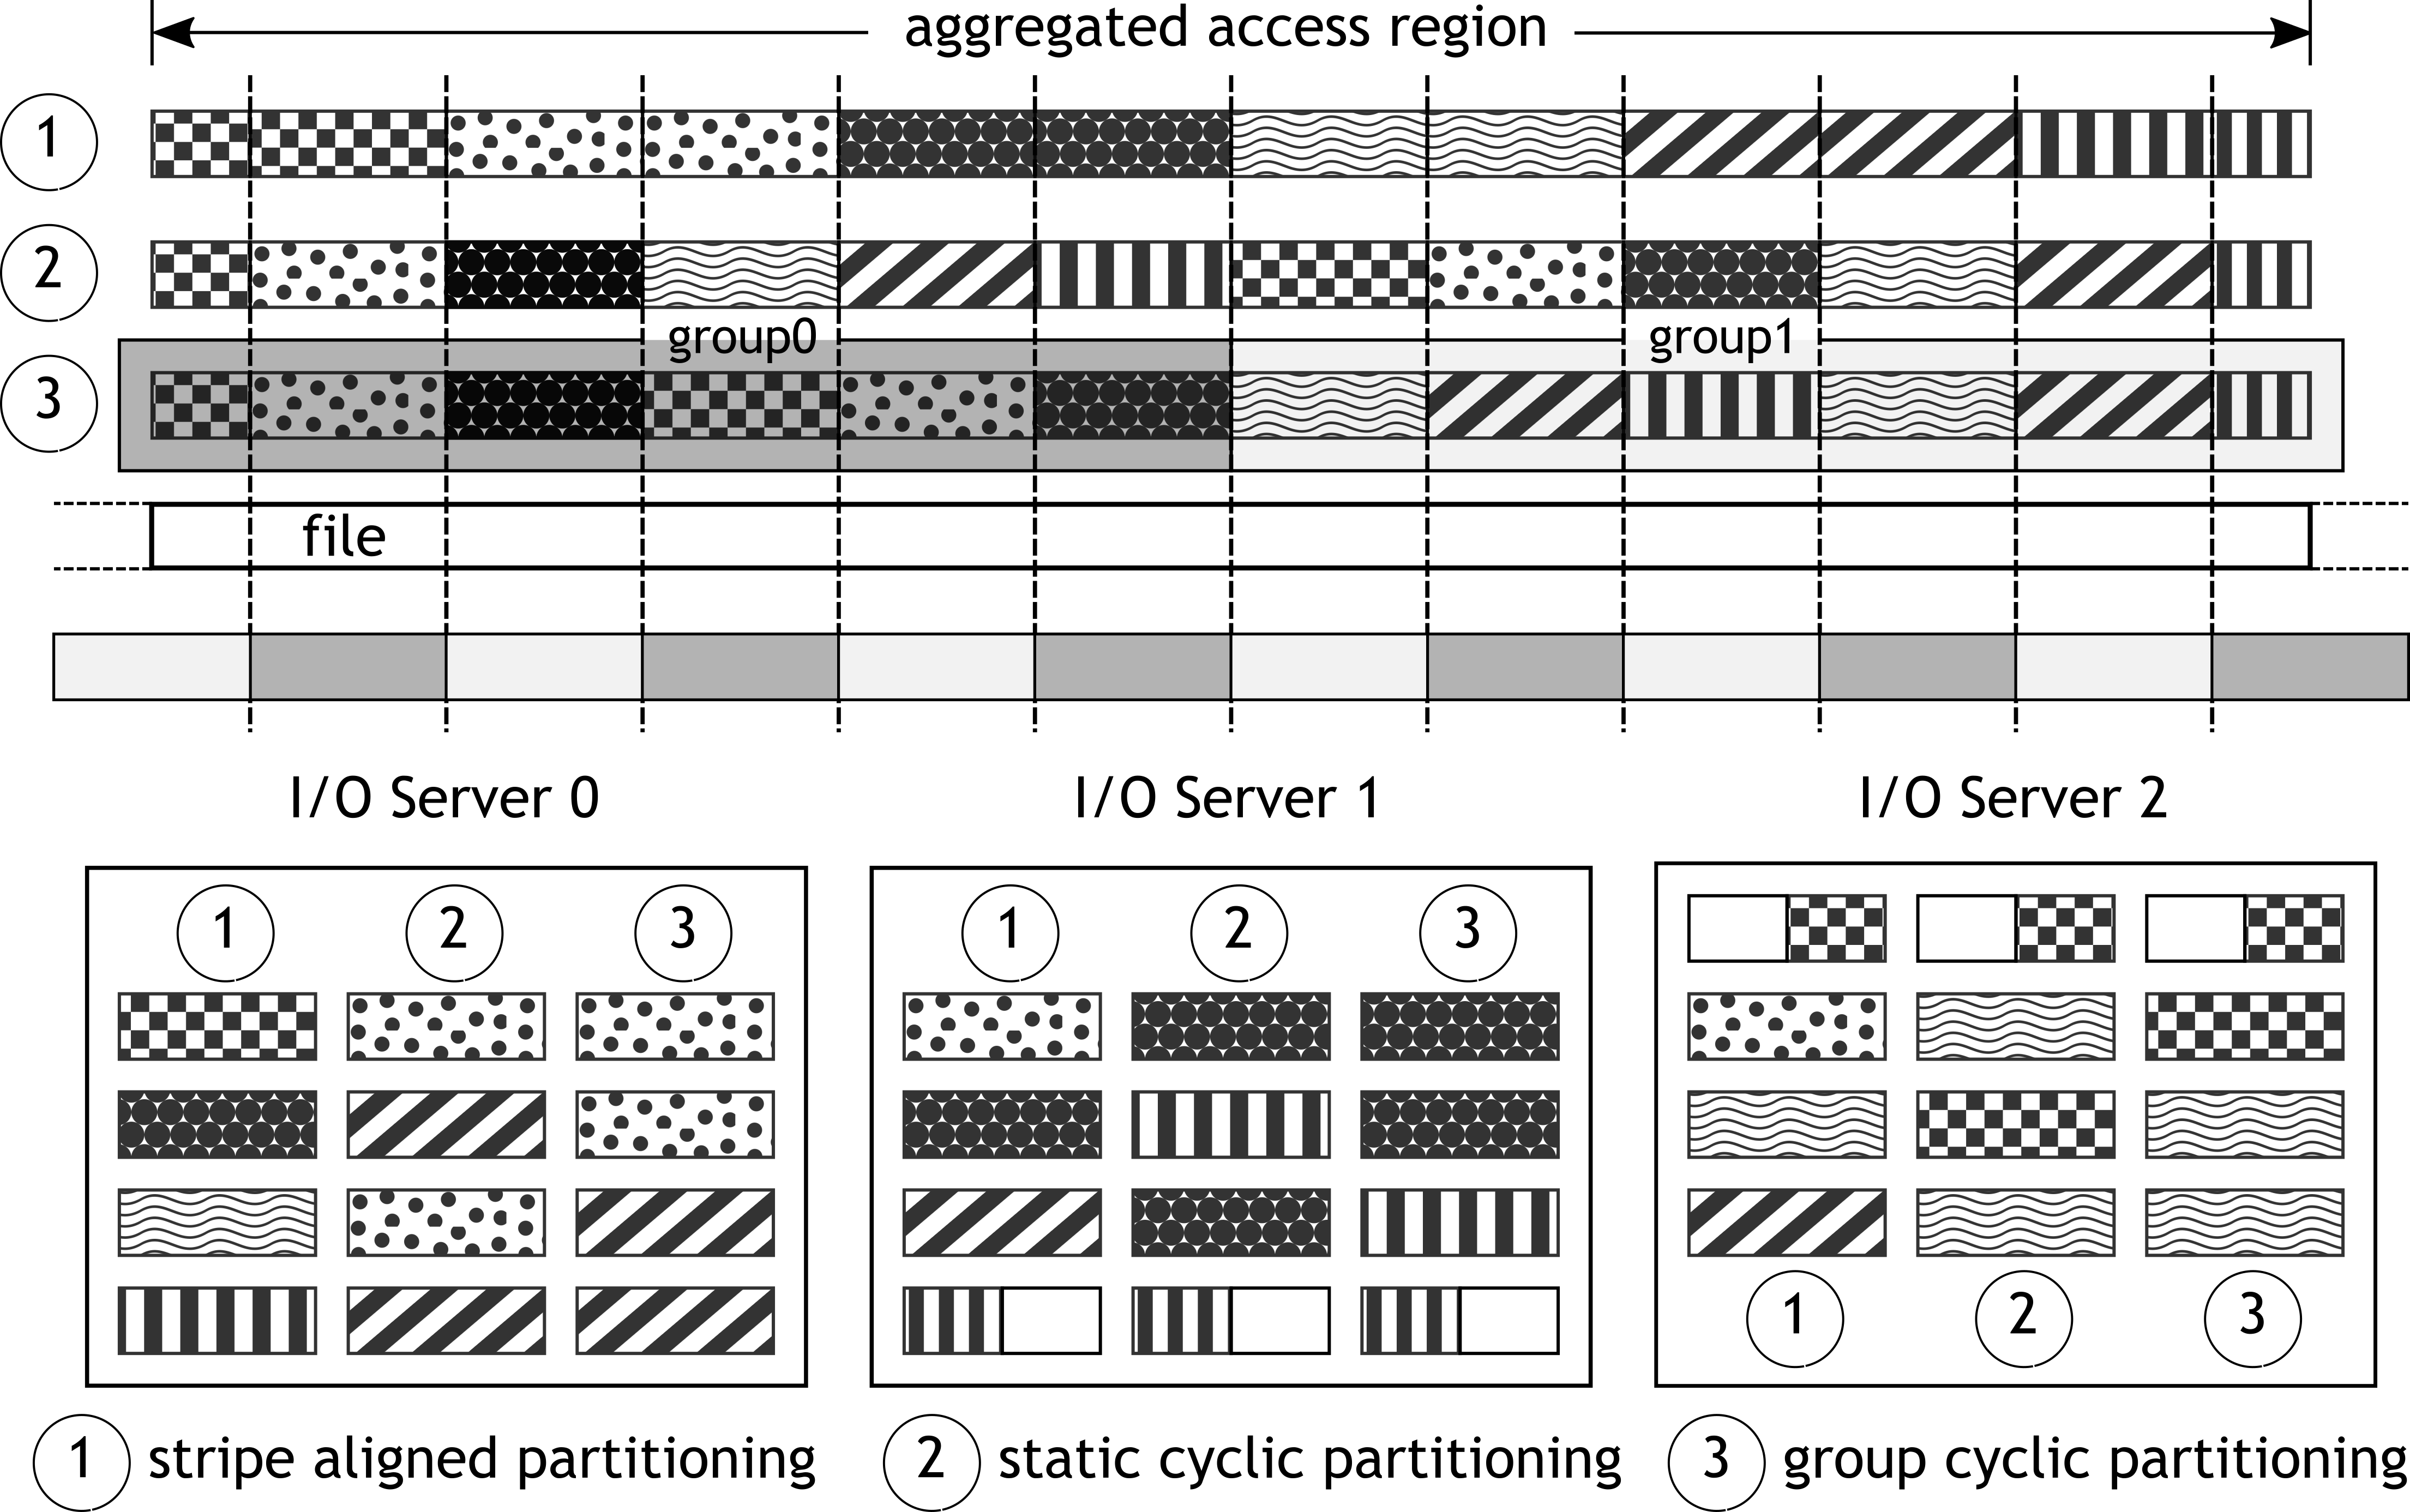
\includegraphics[width=\textwidth]{figures/lustre-partition}
  \caption{}
  \label{figure: lustre-partition}
  \end{subfigure}
  \caption{Possible partitioning strategies for GPFS~\ref{figure: gpfs-partition} and Lustre~\ref{figure: lustre-partition}. File domains, and thus aggregators, are marked with different
  filling patterns.}
\end{figure}

The stripe aligned partitioning works best for GPFS because the token based extent covers the file using the logical offset. For Lustre, on the other hand, the locking protocol depends on how stripes are 
arranged in the I/O servers. Therefore, the stripe aligned strategy causes aggregators to communicate with multiple servers, generating an increased locking protocol overhead. A better partitioning strategy 
would distribute stripes among aggregators in a fixed order, minimizing the communication with multiple servers. This approach is shown in Figure~\ref{figure: lustre-partition} and is called static cyclic 
partitioning. Static cyclic partitioning always assigns stripes to the same aggregator even across multiple I/O operations. This is done by taking the stripe number, dividing it by the number of available 
aggregators and taking the modulo. In this way static cyclic partitioning can also minimize the lock protocol overhead across multiple collective I/O operations. Although static cyclic partitioning can 
reduce locking protocol overhead, it is not yet optimal. To understand why consider case 2 in the figure. In the example, stripes from different aggregators are interleaved in I/O servers. To assign locks 
to each of them the lock manager will need four messages, two for each time the stripes are interleaved. 

A group cyclic partition, as shown in case 3, works better because it arranges stripes belonging to the same aggregator contiguously in the server. In the group cyclic strategy the aggregated access
region is divided into groups, each of these having a number of stripes multiple of the number of I/O servers. Inside each group static cyclic partitioning is then performed to assign stripes to a subset 
of aggregators equal to the number of servers. In the figure, for example, there are three I/O servers and six aggregators. The aggregated access region is therefore divided into two groups. Each group has
six stripes and three aggregators. Using group cyclic partitioning the lock manager only needs two messages to assign the requested locks to the clients.

The interaction between the different file domain partitioning strategies and the locking protocol used by the file system has been studied by Liao and Choudhary~\cite{LiaoA08}~\cite{Liao11}.

\subsection{Logical to Physical Layout Mismatch}
As we have seen in Figure~\ref{figure: lustre-partition} a file in Lustre, as well as in other parallel file systems, is stripped across multiple I/O servers. For this reason the logical file representation
as sequence of blocks does not match the physical layout of data in the parallel file system. We have also shown how this mismatch can affect negatively performance when the file domain partitioning 
strategy does not take into account the characteristics of the locking protocol. More trivially, the logical to physical layout mismatch affects performance because aggregators might request data from more
than one I/O server concurrently. Requests at I/O servers will therefore arrive from multiple clients and because they are served by arrival order the file system cannot guarantee that disk access will
happen sequentially.

In order to have best performance we would therefore need requests at I/O servers to be served by increasing offset. This happens naturally for some specific configuration of I/O pattern when independent
I/O is used over collective I/O; consider the example show in Figure~\ref{figure: resonant-io} as reference. When independent I/O matches the physical layout of data in the file system we have the best
case scenario and correspondingly maximum data transfer performance.

\begin{figure}[!htb]
  \centering
  \includegraphics[width=0.8\textwidth]{figures/resonant-io}
  \caption{Ideal configuration of processes, I/O servers and data distribution in the system.}
  \label{figure: resonant-io}
\end{figure}

The configuration in Figure~\ref{figure: resonant-io} can be easily replicated using collective I/O by building file domains appropriately. This approach has been proposed by several research works
with slight changes and improvements for different type of I/O operations. Zhang et al.~\cite{Zhang2009} have proposed a file domain partitioning scheme to make collective I/O resonant by matching
the logical and physical layout of data in the file system. They also proposed a solution to improve collective read performance by issuing asynchronous read operations and then synchronizing the 
processes in the application. The asynchronous reads work as prefetching hints for the I/O servers. Afterwards, data in the I/O servers is accessed directly by processes, thus avoiding the data 
shuffling phase in the ext2ph algorithm. Chen et al.~\cite{Chen2011} proposed a layout aware collective I/O strategy called LACIO to achieve the same results.

Layout aware strategies require additional information from the file system to discover stripe size and count (how many I/O servers are used to store the file) to build file domains accordingly. 
Because file domains are no longer contiguous in the logical file representation, but are instead contiguous in the physical representation, file system clients cannot access one file domain with a 
single I/O operation; non-contiguous I/O interfaces are therefore required. PVFS supports non-contiguous I/O constructs in the form of list I/O~\cite{Ching2002}~\cite{Ching2003}. The ADIO Lustre 
driver writes one stripe at a time thus avoiding the need for non-contiguous I/O interfaces.

Finally, we mention that a layout aware approach can be also exploited to optimize network communication as done by Filgueira et al.~\cite{Filgueira2008} in their \textit{locality aware two phase I/O}
(LATP I/O) solution.

\subsection{Memory Pressure}
In ROMIO the ext2ph algorithm assigns one aggregator per node by default. This does not take into account the available I/O bandwidth in the node and therefore does not make full utilization of it.
Prediction of different system characteristics at Exascale estimate that node memory will not scale by the same factor as concurrency (i.e., number of cores per node)~\cite{ASCAC2010}, which translates 
into reduced available memory per core. Because collective I/O requires additional buffering resources to shuffle and write data, placing them in nodes without considering memory utilization may translate
into reduced performance due to page reclaiming and swapping to the disk. For this reason, in order to guarantee high performance at large scales we need to consider memory utilization as well. In particular, 
we would like to place aggregators in nodes that have enough memory to accommodate collective I/O buffering requirements and place in every node a sufficient number of aggregators, so that they can saturate the 
available I/O bandwidth. This approach has been explored by Lu et al.~\cite{Lu2012}~\cite{Lu2013}. 

The proposed memory-conscious collective I/O has four components. The first one is an aggregation group division responsible for identifying groups of processes that are isolated and do their aggregation 
independently. This maximises the data movement speed during data shuffle, reducing variance for each aggregator. The second component is an I/O workload partitioning responsible for partitioning the file 
region inside every aggregation group until the ideal file domain size is met. At this point all the hosts have an ideal number of aggregators each with an ideal file domain size that can saturate the host 
I/O bandwidth. However, aggregators' hosts might be short of memory; therefore, a third component, namely the workload portion re-merging, merges the file domains of the hosts that do not have enough memory 
with the neighbour until the memory requirements are met. Finally, inside every host an aggregator allocator assigns aggregators by picking processes that have more data than others in that file domain, 
thus minimizing the amount of data shuffled across the network.

\subsection{Network Concurrency}
Parallel file systems are shared resources accessed concurrently by many processes and possibly different applications. Requests reach I/O servers and are typically served in the order of arrival. This 
means that I/O operations arriving from one application might be interleaved with operations coming from another application. In order to achieve optimal performance all the requests from the same application 
should be served at the same time and every aggregator should spend the same amount of time in the data communication phase. If these conditions are verified, all the aggregators take approximately the same 
time to complete one round of two phase I/O and the total I/O time can be minimized.

\begin{figure}[!htb]
  \centering
  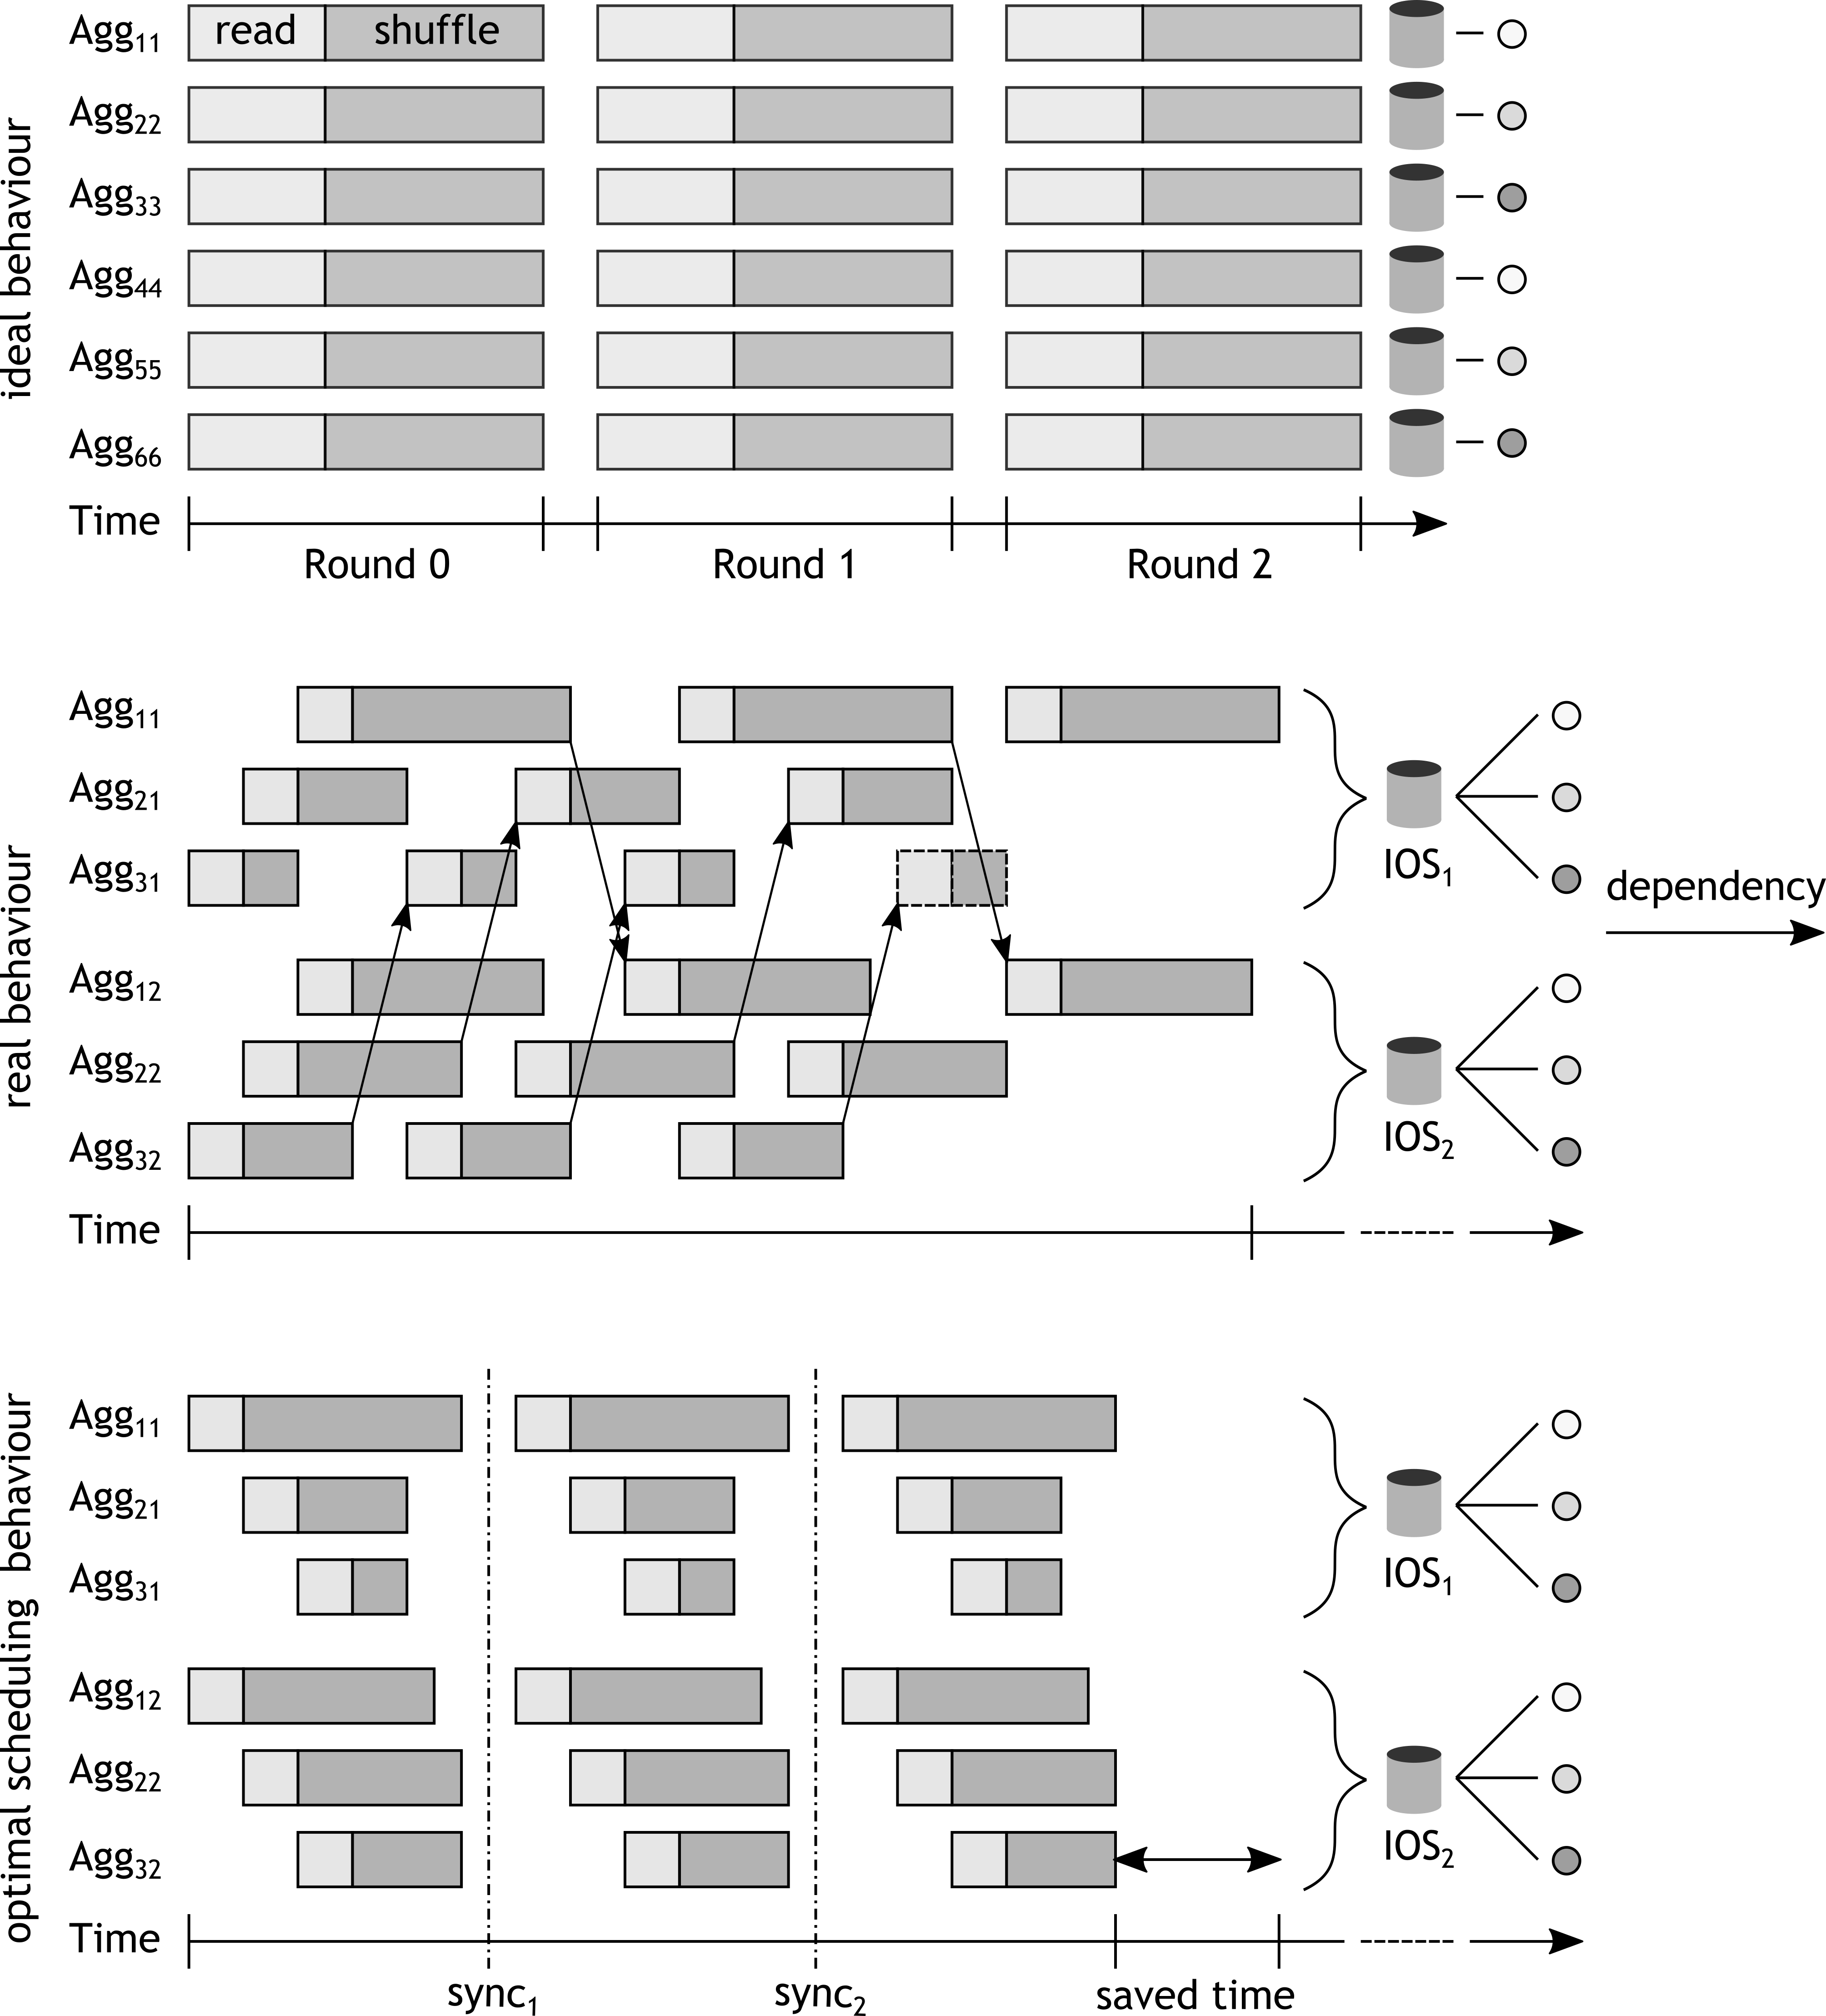
\includegraphics[width=0.8\textwidth]{figures/network-concur}
  \caption{Effect of I/O server scheduling strategies on collective I/O performance. Three examples are shown, in the first every aggregator reads from a different I/O server; in the second three aggregators
  read from the same I/O server, which does not perform any scheduling optimization; and in the third three aggregators read from the same I/O server, which this time does perform a scheduling optimization.}
 % In the figure there are three applications with two aggregators each. In the first example there are six I/O servers. 
 % In the second and third examples there are only two I/O servers, $IOS_1$ and $IOS_2$. $Agg_{11}$ identifies the first aggregator of the first application which reads data from $IOS_1$, $Agg_{12}$ 
 % identifies the second aggregator of the first application which reads data from $IOS_2$, and so on. Every application performs three rounds of two phase I/O. In the `ideal behaviour' every aggregator 
 % reads data from a different I/O server and takes the same time to shuffle data to other processes across the network. In the `real behaviour' aggregators read data only from two I/O servers and take
 % different time to shuffle data. I/O requests in this case are served by arrival order. In the `optimal scheduling behaviour', the slowest aggregator is always served first.}
  \label{figure: network-concur}
\end{figure}

Consider Figure~\ref{figure: network-concur}, showing three applications with two aggregators each and three cases. $Agg_{11}$ identifies the first aggregator of the first application reading data from
$IOS_1$, $Agg_{12}$ identifies the second aggregator of the first application reading data from $IOS_2$, and so on. Every application performs three rounds of two phase I/O. In the `ideal behaviour' every
aggregator reads data from a different I/O server and takes the same time to shuffle data to other processes across the network; in this case all the requests can be ideally scheduled at the same time, giving
the shortest running time for every application. In the `real behaviour' aggregators read data only from two I/O servers and take different time to shuffle data; in this case the shuffle time varies for every
aggregator and is higher for those aggregators that need to exchange data with processes that are placed in a different node. \footnote{When aggregators are served by arrival order and the slowest aggregators always
arrive last, the overall collective I/O time dilates.} In the `optimal scheduling behaviour' the slowest aggregator is always served first; in this case while aggregators are busy shuffling data to other
processes, I/O servers can satisfy following read requests, thus overlapping network communication and I/O time, minimizing the runtime for all applications.
%The first case describes the scenario in which every aggregator requests data from a different 
%I/O server and the shuffle time is the same for each of them. In this case all the requests can be ideally scheduled at the same time giving the shortest running time for every application. The second 
%case describes an example of what the real behaviour may look like. In particular, the shuffle time in this case varies for every aggregator and is higher for aggregators that need to exchange data with 
%processes that are placed in other nodes compared to aggregators that only need to exchange data with processes located in the same node. When aggregators are served by arrival order and slowest aggregators 
%always arrive last, the overall collective I/O time dilates. The third case describes what happens when slowest aggregators are always scheduled first. In this case, while aggregators are busy shuffling 
%data to other processes, I/O servers can satisfy following read requests, thus overlapping network communication time and I/O, minimizing the runtime of all applications.

Liu et al.~\cite{Liu2013} have proposed a new scheduling algorithm for PVFS servers that takes into account the shuffle cost of aggregators across multiple applications and always schedules the slowest
aggregators first, thus achieving the slowest average running time for all of them. This optimization only works for collective read operations. Indeed, for writes the shuffle phase happens before the 
I/O phase. In order to implement the same strategy for write operations, one could use a double buffering approach to pipeline data shuffling and writes. This solution has been proposed by Sehrish et al.
~\cite{Sehrish2013}.

\subsection{Global Synchronization Overhead}
As we have previously discussed in the ext2ph algorithm collective I/O performance is negatively impacted by global synchronization. Collective MPI constructs are used to coordinate processes
in the application and to exchange state during multiple rounds of data shuffling and I/O. Nevertheless, there are cases in which the input domain decomposition, and thus the distribution
of requests in the file, does not require to globally synchronize all processes but only smaller groups of them. These I/O patterns can be exploited to reduce the global synchronization overhead.
Figure~\ref{figure: parcol} shows an example of six processes participating in a collective write operation. In the example there are four aggregators and, as we can see, two groups of three processes
exchange data with only two aggregators.

\begin{figure}[!htb]
  \centering
  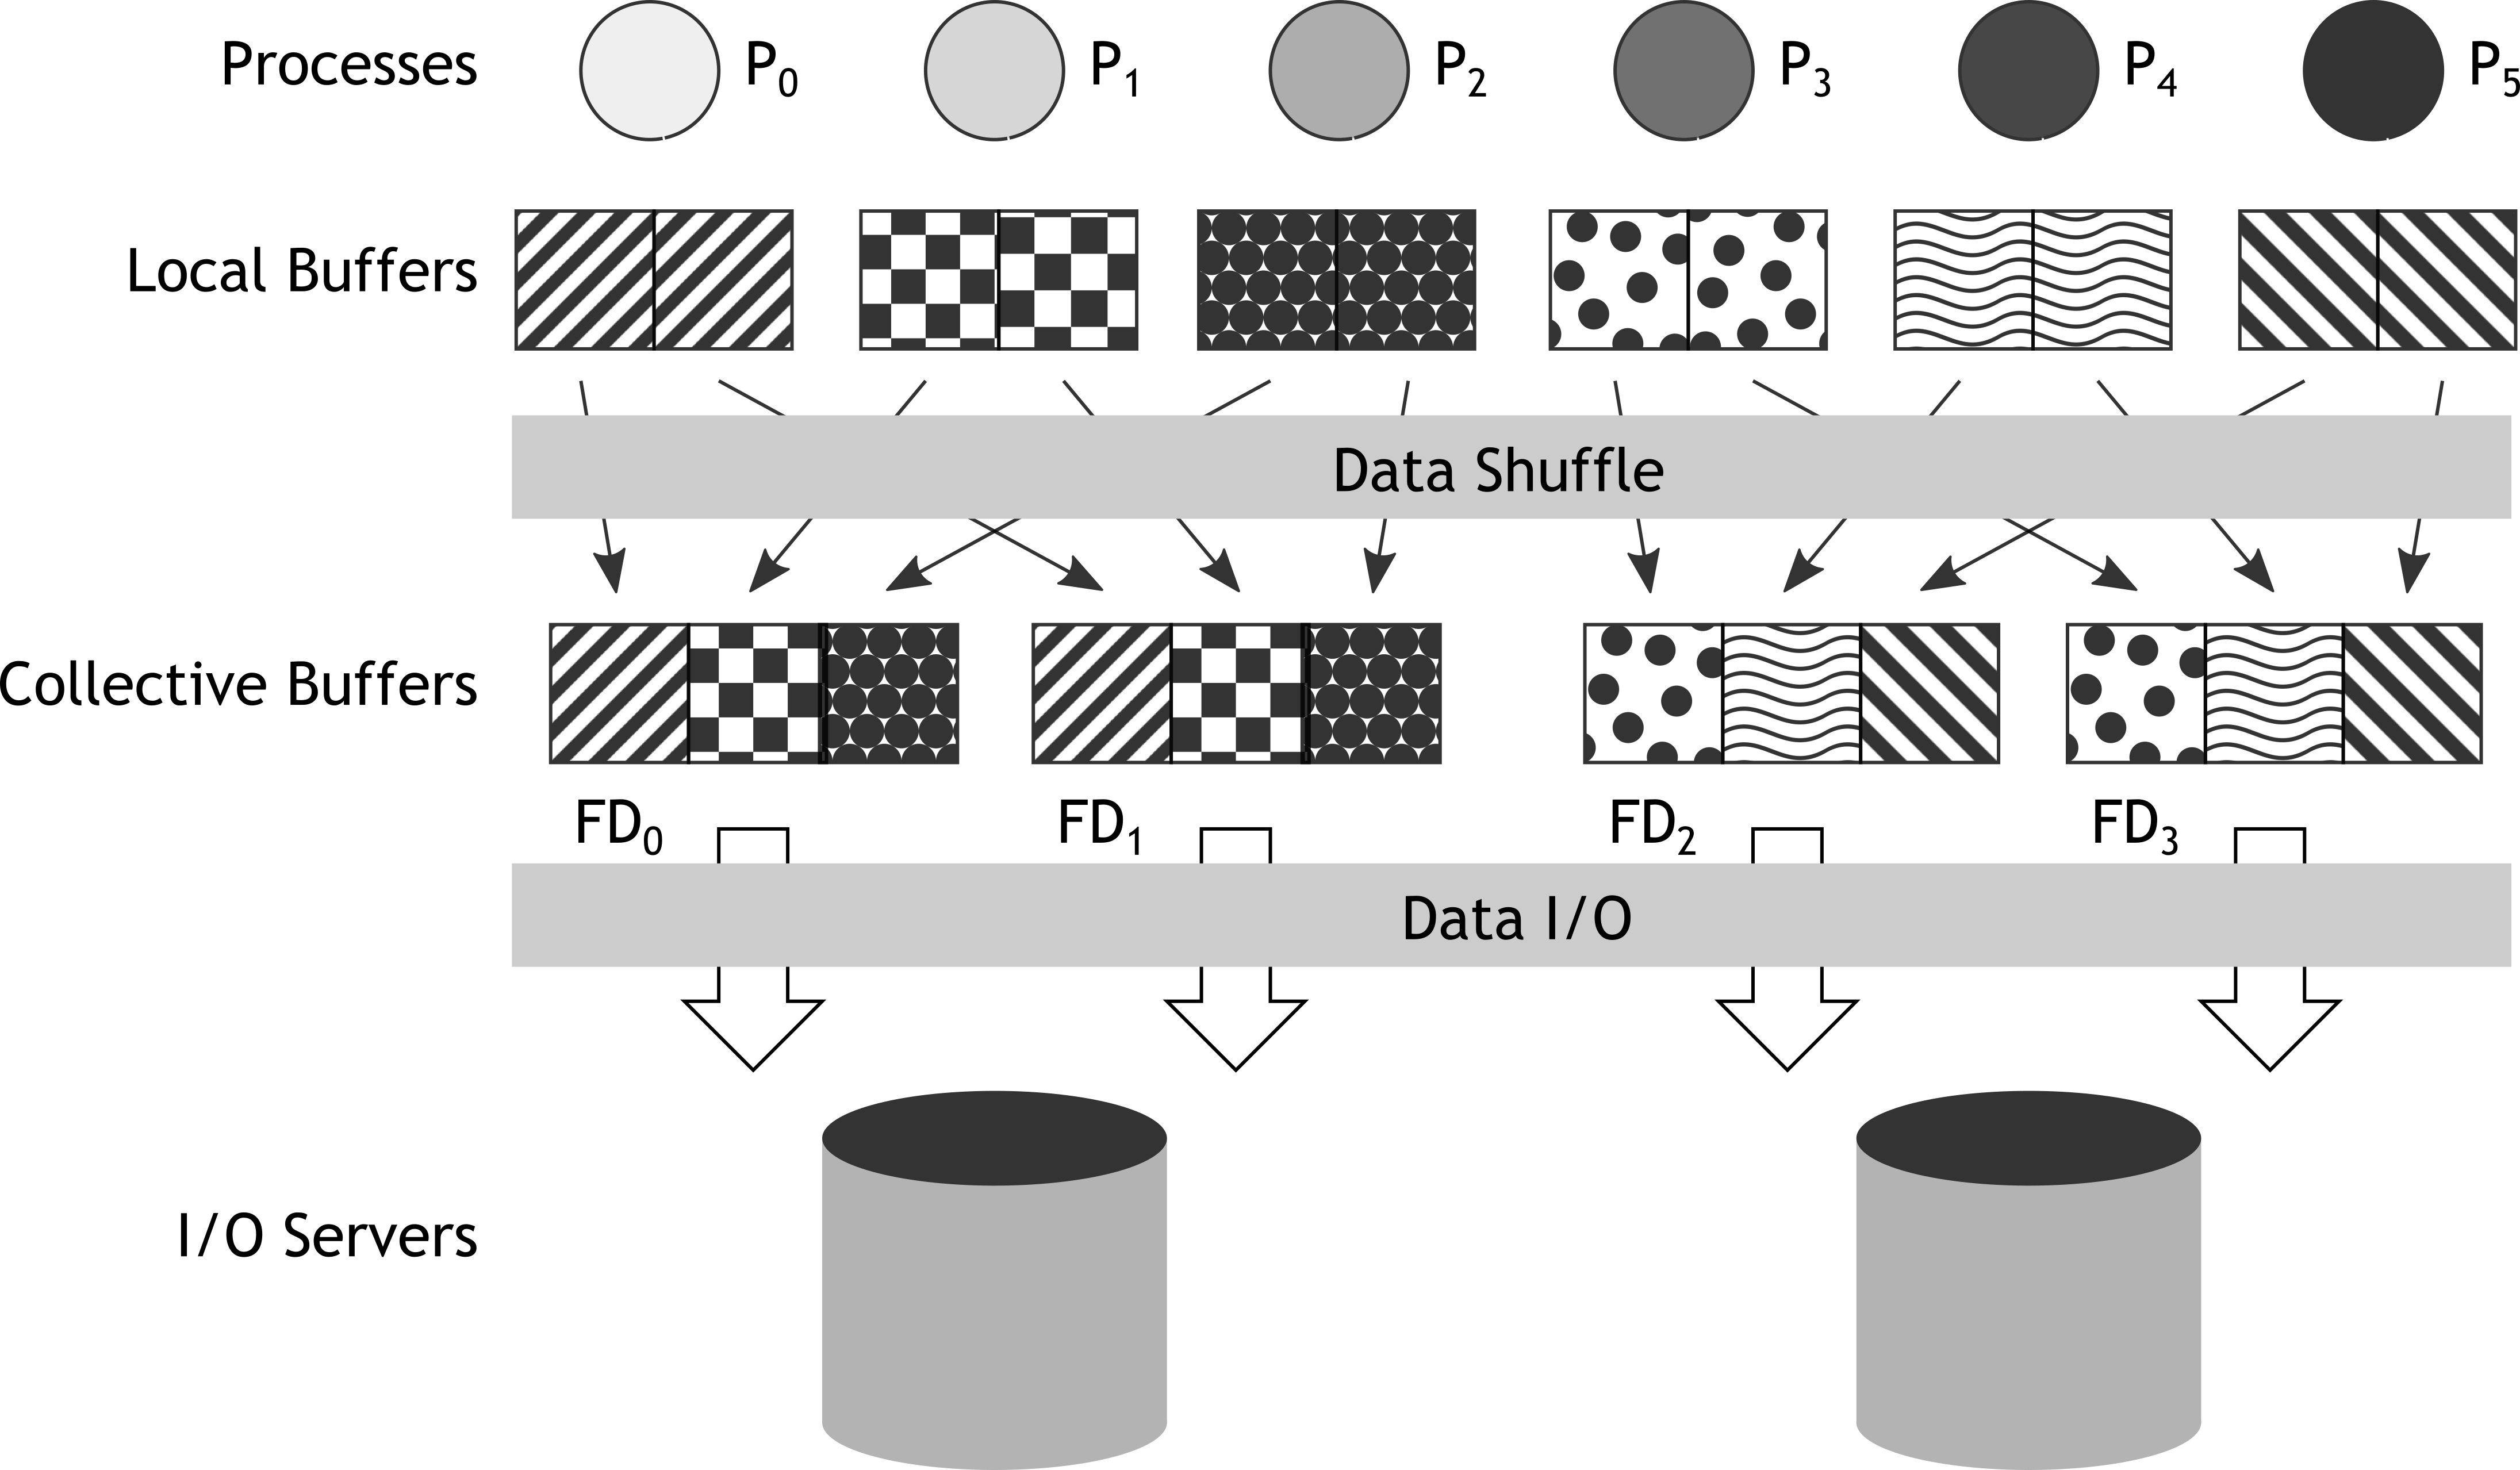
\includegraphics[width=0.8\textwidth]{figures/parcoll}
  \caption{Six processes are collaborating in collective I/O. Because $P_0$, $P_1$ and $P_2$ do not exchange data with other processes there is no need for them to communicate data shuffling information
  to $P_3$, $P_4$ and $P_5$ during two phase I/O rounds.}
  \label{figure: parcol}
\end{figure}

This observation has been exploited by Yu and Vetter~\cite{Yu08} to partition collective I/O into smaller groups of processes that coordinate independently from each other, that is, in the ext2ph
implementation these processes can use different communicators when exchanging data shuffling information with \texttt{MPI\_Alltoall()} (refer to Figure~\ref{figure: coll_io_impl}). Because 
some I/O patterns do not allow the partitioning of processes, they convert the original I/O pattern using an intermediate file view and rearrange data in the file to match the intermediate pattern. This 
approach works but has considerable limitations. In particular, if the file is written using a certain number of processes and aggregators, the original input can be reconstructed only if data in the file 
is read using the same number of processes and aggregators. The reason is that MPI-IO does not define a binary format. Data is written using byte information and in order to reconstruct the intermediate
file view the collective I/O configuration must be the same. The immediate limitation of this approach is that if data is written for checkpoint/restart purposes, the application cannot be restarted using a 
different number of processes because read and write layout would not match.

\section{A Non-Volatile Memory Based Approach} \label{sec: nvm-approach}
As we have discussed in Section~\ref{sec: coll_io_limit}, collective I/O performance is limited by the slowest aggregators run-time. This is mainly due to the fact that the parallel 
file system is shared among many applications in the cluster and requests coming from the same application are not served simultaneously by all I/O servers. This, in conjunction with 
the need for global synchronization at the beginning of every phase of data shuffle and I/O, contributes to the suboptimal performance in large scale clusters. In this work we focus 
on write performance improvements since HPC simulation codes are write intensive; while read operations are typically limited to loading of initialization parameters that are used 
during the simulation. Our approach focuses on global synchronization overhead reduction in the extended two phase algorithm. We achieve our goal by taking advantage of non-volatile 
memory devices, more specifically SSDs, in compute nodes. 

Instead of performing collective I/O to the global parallel file system directly, we perform collective I/O to the local NVM storage and then move data to the global file system asynchronously 
(i.e., in the background), allowing the application to continue with useful work. Data synchronization is not performed collectively but instead independently. This effectively converts collective 
I/O to the parallel file system into independent I/O, taking the parallel file system out of the collective I/O critical path. Since local NVM storage devices are not shared with other nodes, I/O 
requests can be served almost simultaneously, thus reducing the I/O response time in aggregators and limiting the amount of time spent in global synchronization operations. Our approach also benefits 
the memory pressure on compute nodes because we can achieve high performance using smaller collective buffers.

In this section we present the high-level architecture of the ROMIO implementation of MPI-IO as well as our proposed design. The two are shown in Figure~\ref{figure: romio-architecture} 
and~\ref{figure: new-romio-architecture} respectively. The ROMIO middleware is designed to be modular and easily extensible. Support for different parallel file systems is provided through 
additional software modules called drivers. The appropriate driver is selected at file open time through the ADIO interface, following an approach similar to the Virtual File System layer 
of the Linux Kernel.

\begin{figure}[!htb]
  \centering
  \begin{subfigure}[t]{0.38\textwidth}
  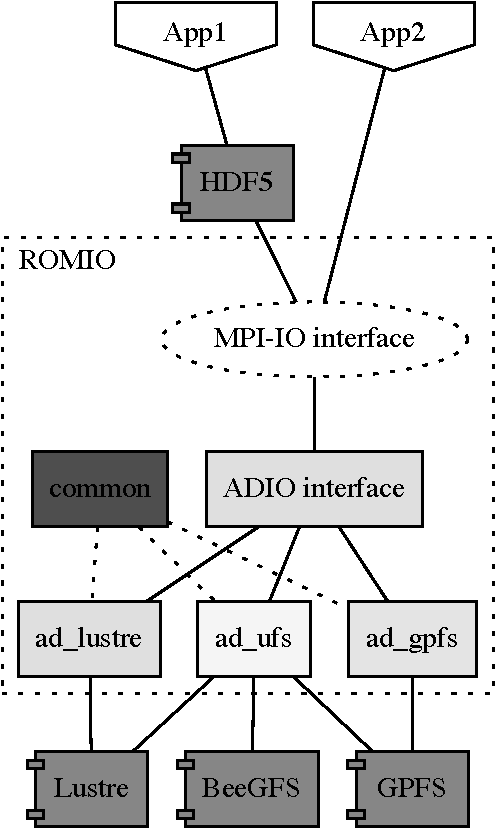
\includegraphics[width=\textwidth]{figures/romio-architecture-baw.pdf}
  \caption{}
  \label{figure: romio-architecture}
  \end{subfigure}
  \begin{subfigure}[t]{0.55\textwidth}
  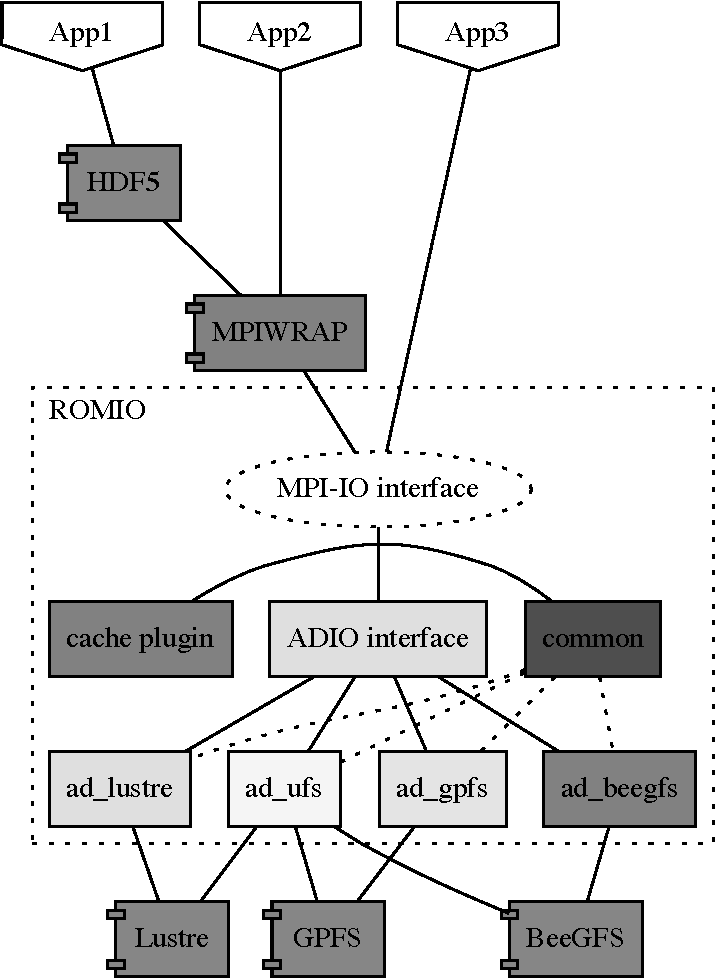
\includegraphics[width=\textwidth]{figures/new-romio-architecture-baw.pdf}
  \caption{}
  \label{figure: new-romio-architecture}
  \end{subfigure}
  \caption{Original ROMIO architecture (\ref{figure: romio-architecture}) and proposed ROMIO architecture (\ref{figure: new-romio-architecture}).}
\end{figure}

In Figure~\ref{figure: romio-architecture} there are three different file system drivers: \textit{ad\_gpfs} for GPFS support, \textit{ad\_ufs} for \textit{universal file system} (UFS) 
support, and \textit{ad\_lustre} for Lustre support. These drivers share features implemented in the \textit{common} module. The common module contains the implementation for most of 
the I/O operations used by the UFS driver (ad\_ufs) and other drivers. File system drivers can implement their own version of I/O operations or use the ones made available by the common 
module. Lustre, for example, uses the common collective open operation (\codeword{ADIOI\_GEN\_Opencoll()}) but implements its own collective write operation (\codeword{ADIOI\_LUSTRE\_WriteStridedColl()}). 
Specific implementations are selected using a file operation table that has to be defined by every file system driver. Listing~\ref{list: lustre_table} shows the operation table for the \textit{ad\_lustre} 
driver.

\begin{lstlisting}[language=C, caption=Operation table for Lustre driver., label={list: lustre_table}]
struct ADIOI_Fns_struct ADIO_LUSTRE_operations = {
    ADIOI_LUSTRE_Open,             /* Open */
    ADIOI_GEN_OpenColl,            /* OpenColl */
    ADIOI_LUSTRE_ReadContig,       /* ReadContig */
    ADIOI_LUSTRE_WriteContig,      /* WriteContig */
    ADIOI_GEN_ReadStridedColl,     /* ReadStridedColl */
    ADIOI_LUSTRE_WriteStridedColl, /* WriteStridedColl */
    ADIOI_GEN_SeekIndividual,      /* SeekIndividual */
    ADIOI_GEN_Fcntl,               /* Fcntl */
    ADIOI_LUSTRE_SetInfo,          /* SetInfo */
    ADIOI_GEN_ReadStrided,         /* ReadStrided */
    ADIOI_LUSTRE_WriteStrided,     /* WriteStrided */
    ADIOI_GEN_Close,               /* Close */
#if defined(ROMIO_HAVE_WORKING_AIO) && !defined(CRAY_XT_LUSTRE)
    ADIOI_GEN_IreadContig,         /* IreadContig */
    ADIOI_GEN_IwriteContig,        /* IwriteContig */
#else
    ADIOI_FAKE_IreadContig,        /* IreadContig */
    ADIOI_FAKE_IwriteContig,       /* IwriteContig */
#endif
    ADIOI_GEN_IODone,              /* ReadDone */
    ADIOI_GEN_IODone,              /* WriteDone */
    ADIOI_GEN_IOComplete,          /* ReadComplete */
    ADIOI_GEN_IOComplete,          /* WriteComplete */
    ADIOI_GEN_IreadStrided,        /* IreadStrided */
    ADIOI_GEN_IwriteStrided,       /* IwriteStrided */
    ADIOI_GEN_Flush,               /* Flush */
    ADIOI_GEN_Resize,              /* Resize */
    ADIOI_GEN_Delete,              /* Delete */
    ADIOI_GEN_Feature,             /* Features */
    "LUSTRE:",
};
\end{lstlisting}

In Figure~\ref{figure: new-romio-architecture} we extend the presented ROMIO architecture with two additional modules: a dedicated driver supporting the BeeGFS file system 
(\textit{ad\_beegfs}) and a \textit{cache plugin} that links directly to the common module, thus providing NVM caching features to all the underlying file system drivers. Indeed,
most of the file system drivers supported in ROMIO use the common implementation of the basic I/O functionalities like, for example, \codeword{ADIOI\_GEN\_OpenColl()} to collectively 
open a file, \codeword{ADIO\_Close()} to collectively close a file, and \codeword{ADIOI\_GEN\_WriteContig()} to write a contiguous extent of data to the file using the POSIX write 
operation. Furthermore, we have also developed an external library called \textit{MPIWRAP} that is used to allow transparent integration of the new caching functionalities into existing 
applications without any need of modifying them. 

\subsection{MPI-IO Hints Extensions}
In order to take advantage of attached non-volatile memories in compute nodes we have introduced a new set of MPI-IO hints, reported in Table~\ref{table: hints_table}, and a 
corresponding set of modifications in the ROMIO implementation of the common layer supporting them.

\begin{table}[!htb]
\centering
\ra{1.5}
\caption{Proposed MPI-IO hints extensions.}
\newcolumntype{K}{>{\centering\arraybackslash} m{4.2cm}}
\newcolumntype{V}{>{\centering\arraybackslash} m{5cm}}
\begin{tabular}{KV}
\toprule
\bf \small Hint & \bf \small Value \\
\midrule
\small \codeword{e10\_cache} & \small \codeword{enable}, \codeword{disable}, \codeword{coherent}\\
\small \codeword{e10\_cache\_path} & \small cache directory pathname\\
\small \codeword{e10\_cache\_flush\_flag} & \small \codeword{flush\_immediate}, \codeword{flush\_onclose}, \codeword{flush\_none}\\
\small \codeword{e10\_cache\_discard\_flag} & \small \codeword{enable}, \codeword{disable}\\
\small \codeword{e10\_cache\_threads} & \small number of synchronization thread in pool\\
\small \codeword{ind\_wr\_buffer\_size} & \small synchronization buffer size [bytes]\\
\hline
\end{tabular}
\label{table: hints_table}
\end{table}

The new hints are used to control the data path in the storage system as well as to define a basic set of cache policies for synchronization and space management. In particular, 
the \codeword{e10\_cache} hint is used to \codeword{enable} or \codeword{disable} the cache, directing applications' data to the local file system instead of the global file system. 
When the hint is set to \codeword{coherent} all the written data extents are locked until cache synchronization is completed. This prevents other processes from modifying the same
data before this is persisted in the global file system. The \codeword{e10\_cache\_path} hint is used to control where, in the local file system tree, the cache file will reside. 
The \codeword{e10\_cache\_flush\_flag} hint is used to control the synchronization policy of cached data to the global file. If the hint is set to \codeword{flush\_immediate} data 
is immediately flushed to the global file. Alternatively, if the hint is set to \codeword{flush\_onclose} data is flushed to the global file when it is closed. A \codeword{flush\_none} 
option is also available to keep data local to the node and never flush it to the global file system. This might be used in the case the user does not wish to flush every checkpoint to the
global file system. The \codeword{e10\_cache\_discard\_flag} hint is used to perform basic cache space management. In particular, if the hint is set to \codeword{enable} the cache file 
is removed after closed, otherwise (\codeword{disable}) it is retained until the user manually removes it. The \codeword{e10\_cache\_threads} hint is used to communicate to the implementation 
the number of threads to be created in the synchronization thread pool when the file is opened (default is 1). Finally, the \codeword{ind\_wr\_buffer\_size} hint controls the size of the 
buffer used to synchronize cached data to the global file. This hint already existed in ROMIO but was only used during independent I/O to determine the write granularity. The hints in 
Table~\ref{table: hints_table} can be used in conjunction with the collective I/O hints described in Table~\ref{table: coll_io_hints_table} of Chapter~\ref{chapt: background}.

Besides the proposed cache policies, more complex ones are possible. For example, the cache synchronization could take into account the level of congestion of the I/O servers. The cache 
replacement policy could also use a more complex strategy to evict cached files (or extents of data inside the file). Although these can be implemented in ROMIO, they introduce more 
sophisticated functionalities that are beyond the scope of this work. Here, our goal is to demonstrate the benefit that the employment of NVM devices in compute nodes can have on parallel
I/O performance.

\subsection{Cache Hints Integration in ROMIO}
As already mentioned, the introduced MPI-IO hints are supported by a corresponding set of modifications in the ROMIO implementation\footnote{\url{http://www.github.com/gcongiu/E10.git}},
which come in the form of cache plugin. The proposed cache plugin class diagram is shown in Figure~\ref{figure: cache-plugin-class}. The cache plugin provides all the functionalities 
necessary to handle the additional cache layer. In the figure there are three main software components: 

\begin{itemize}
\item a synchronization thread object that takes care of moving data from the local to the global file system;
\item a synchronization request object used to describe what data should be moved and finally;
\item an atomic queue object that makes up the communication channel between main and synchronization threads. 
\end{itemize}

In order to handle the cache file properly we have also extended the \codeword{MPI\_File} opaque object with two additional attributes, a cache file handle named \codeword{cache\_fd} and 
an array of pointers to available synchronization thread instances named \codeword{thread\_pool}.

\begin{figure}[!htb]
  \centering
  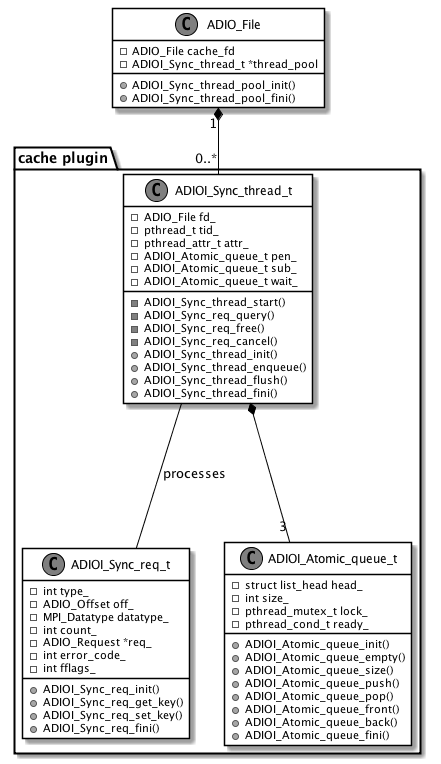
\includegraphics[width=0.6\textwidth]{figures/cache_architecture}
  \caption{Cache plugin class diagram. The synchronization thread \codeword{ADIOI\_Sync\_thread\_t} serves synchronization requests of type \codeword{ADIOI\_Sync\_req\_t}.}
  \label{figure: cache-plugin-class}
\end{figure}

Moreover, we have added two functions, \codeword{ADIOI\_Sync\_thread\_pool\_init()} and \codeword{ADIOI\_Sync\_thread\_pool\_fini()}, to initialize and finalize the thread pool.
In the following we describe in detail the three software components just introduced and explain how they work together.

\subsubsection{Cache Synchronization Thread}
The \codeword{ADIOI\_Sync\_thread\_t} object provides the infrastructure to initialize/finalize threads and to enqueue, flush and wait for synchronization requests. A pool of synchronization threads 
is created when the file is opened with \codeword{MPI\_File\_open()} and destroyed when the file is closed with \codeword{MPI\_File\_close()}. The synchronization thread object has six attributes: 
the \codeword{fd\_} attribute is a pointer to the internal ROMIO representation of the MPI file object and is used by the thread to retrieve all the information it requires to perform its tasks 
(e.g., POSIX file descriptors) without having to pass such information through the synchronization request object; the \codeword{tid\_} attribute is the POSIX thread identifier and is used by the 
main thread in the \codeword{pthread\_join()} operation when the file is closed; the \codeword{attr\_} are the POSIX thread attributes; finally there are three queues, a submission queue named 
\codeword{sub\_} that contains requests that are ready to be served, a pending queue named \codeword{pen\_} that contains requests that are not yet ready to be served, and a wait queue named 
\codeword{wait\_} that contains a copy of every request that is in the submission queue and is used by the main thread to check status of submitted requests.

%\begin{lstlisting}[language=C, caption=Synchronization Thread API, label={list: sync-thread}]
%%/* Used by ADIOI_Sync_req_init() method */
%enum {
%  ADIOI_THREAD_SYNC = 0,
%  ADIOI_THREAD_SHUTDOWN
%};
%
%/* Synchronization Thread Object Definition */
%struct ADIOI_Sync_thread {
%  ADIO_File            fd_;
%  pthread_t            tid_;
%  pthread_attr_t       attr_;
%  ADIOI_Atomic_queue_t sub_;
%  ADIOI_Atomic_queue_t pen_;
%  ADIOI_Atomic_queue_t wait_;
%};
%
%/* Synchronization Thread Opaque Object */
%typedef struct ADIOI_Sync_thread *ADIOI_Sync_thread_t;
%
%/* Synchronization Thread Public APIs */
%int  ADIOI_Sync_thread_init(ADIOI_Sync_thread_t *, ...);
%int  ADIOI_Sync_thread_fini(ADIOI_Sync_thread_t *);
%void ADIOI_Sync_thread_enqueue(ADIOI_Sync_thread_t, ADIOI_Sync_req_t);
%void ADIOI_Sync_thread_flush(ADIOI_Sync_thread_t);
%void ADIOI_Sync_thread_wait(ADIOI_Sync_thread_t);
%\end{lstlisting}

The public interface of the synchronization thread provides two methods to initialize and destroy the thread object and three additional methods: \codeword{ADIOI\_Sync\_thread\_enqueue()} used by 
the main thread to enqueue new requests in the pending queue, \codeword{ADIOI\_Sync\_thread\_flush()} used by the main thread to move requests from the pending queue to the submission queue, thus
allowing the thread to serve them, and finally \codeword{ADIOI\_Sync\_thread\_wait()} used by the main thread to wait for all the submitted requests to complete. The thread object also contains
four additional internal methods that are not directly visible to the main thread and are used to implement the supported services through the MPI generalized request interface~\cite{mpispecs}.

\subsubsection{Cache Synchronization Request}
The \codeword{ADIOI\_Sync\_req\_t} object provides the infrastructure required to initialize/finalize, set/get attributes to/from synchronization requests. Synchronization requests are initialized 
by the main thread in the \codeword{ADIO\_GEN\_WriteContig()} function and submitted to synchronization threads which will satisfy them while the main thread can progress with its work. 
The synchronization request object has seven attributes: the \codeword{type\_} attribute specifies the type of the request, either \codeword{ADIOI\_THREAD\_SYNC} or \codeword{ADIOI\_THREAD\_SHUTDOWN};
the first is used to describe a written file extent that needs to be copied from the cache to the global file system, while the second is used to shut down the synchronization thread when the thread 
is no longer needed; the \codeword{count\_} attribute represents the number of elements of type \codeword{datatype\_} to be transfered, while the initial position of these in the file is defined
by the \codeword{offset\_} attribute; the \codeword{fflags\_} attribute tells the synchronization thread when data should be transfered; the \codeword{req\_} attribute is a MPI request handle and is 
used by the main thread to check the synchronization status of the request by invoking \codeword{MPI\_Wait()}; finally, the \codeword{error\_code\_} attribute is used by the synchronization thread to 
set the return code that is afterwards interpreted by the main thread.

%\begin{lstlisting}[language=C, caption=Synchronization Request Attributes and Public API., label={list: sync-req}]
%/* Used by ADIOI_Sync_req_{get,set}_key() methods */
%enum {
%  ADIOI_SYNC_TYPE = 0, /* sync req type        */
%  ADIOI_SYNC_OFFSET,   /* sync req write off   */
%  ADIOI_SYNC_DATATYPE, /* sync req datatype    */
%  ADIOI_SYNC_COUNT,    /* sync req count       */
%  ADIOI_SYNC_REQ,      /* sync req MPI_Request */
%  ADIOI_SYNC_ERR_CODE, /* sync req error_code  */
%  ADIOI_SYNC_FFLAGS,   /* sync req flush flag  */
%  ADIOI_SYNC_ALL,      /* sync req all fields  */
%  ADIOI_SYNC_REQ_ERR   /* sync req err code    */
%};
%
%/* Synchronization Request Object Definition */
%struct ADIOI_Sync_req {
%  int           type_;
%  int           count_;
%  int           error_code_;
%  int           fflags_;
%  ADIO_Offset   off_;
%  MPI_Datatype  datatype_;
%  MPI_Request  *req_;
%};
%
%/* Synchronization Request Opaque Object */
%typedef struct ADIOI_Sync_req *ADIOI_Sync_req_t;
%
%/* Synchronization Request Public APIs */
%int ADIOI_Sync_req_init(ADIOI_Sync_req_t *, ...);
%int ADIOI_Sync_req_fini(ADIOI_Sync_req_t *);
%int ADIOI_Sync_req_get_key(ADIOI_Sync_req_t, ...);
%int ADIOI_Sync_req_set_key(ADIOI_Sync_req_t, ...);
%\end{lstlisting}

The public interface of the synchronization request object provides two methods to initialize and destroy the synchronization request object, a get method named \codeword{ADIOI\_Sync\_req\_get\_key()} 
and a set method named \codeword{ADIOI\_Sync\_req\_set\_key()}. 

\subsubsection{Atomic Queue}
The \codeword{ADIOI\_Atomic\_queue\_t} object provides the communication channel between the main thread and the synchronization thread enforcing atomicity through POSIX mutual exclusion constructs.
The atomic queue object has four attributes: the \codeword{head\_} attribute is a pointer to the head of a double linked list used to implement the queue\footnote{We used the Linux kernel implementation
of the double linked list.}; the \codeword{size\_} stores the number of elements currently present in the queue; the \codeword{lock\_} attribute is a POSIX mutex used to ensure internal data structure 
consistency during queue manipulation; finally, the \codeword{ready\_} attribute is a condition variable used by the main thread to signal the synchronization thread that the queue is no longer empty. 

%\begin{lstlisting}[language=C, caption=Atomic Queue Attributes and Public API., label={list: atomic-queue}]
%/* Atomic Queue Object Definition */
%struct ADIOI_Atomic_queue {
%  struct list_head head_;
%  int              size_;
%  pthread_mutex_t  lock_;
%  pthread_cond_t   ready_;
%};
%
%/* Atomic Queue Opaque Object */
%typedef struct ADIOI_Atomic_queue *ADIOI_Atomic_queue_t;
%
%/* Atomic Queue Public APIs */
%void ADIOI_Atomic_queue_init(ADIOI_Atomic_queue_t *);
%void ADIOI_Atomic_queue_fini(ADIOI_Atomic_queue_t *);
%int  ADIOI_Atomic_queue_empty(ADIOI_Atomic_queue_t);
%int  ADIOI_Atomic_queue_size(ADIOI_Atomic_queue_t);
%ADIOI_Sync_req_t ADIOI_Atomic_queue_front(ADIOI_Atomic_queue_t);
%ADIOI_Sync_req_t ADIOI_Atomic_queue_back(ADIOI_Atomic_queue_t);
%void ADIOI_Atomic_queue_push(ADIOI_Atomic_queue_t,   ADIOI_Sync_req_t);
%void ADIOI_Atomic_queue_pop(ADIOI_Atomic_queue_t);
%\end{lstlisting}

The atomic queue object supports the standard queue APIs\footnote{http://www.cplusplus.com/reference/queue/queue/?kw=queue} and thus we do not give a description for them here.

\subsubsection{Collective Write Caching}
Now that we have described all the cache plugin components, we can explain how the cache plugin works in collective write operations. Figure~\ref{figure: coll_io_cache} shows the flow diagram
obtained by extending the diagram in Figure~\ref{figure: coll_io_impl} with the cache plugin. 
\begin{figure}[H]
  \centering
  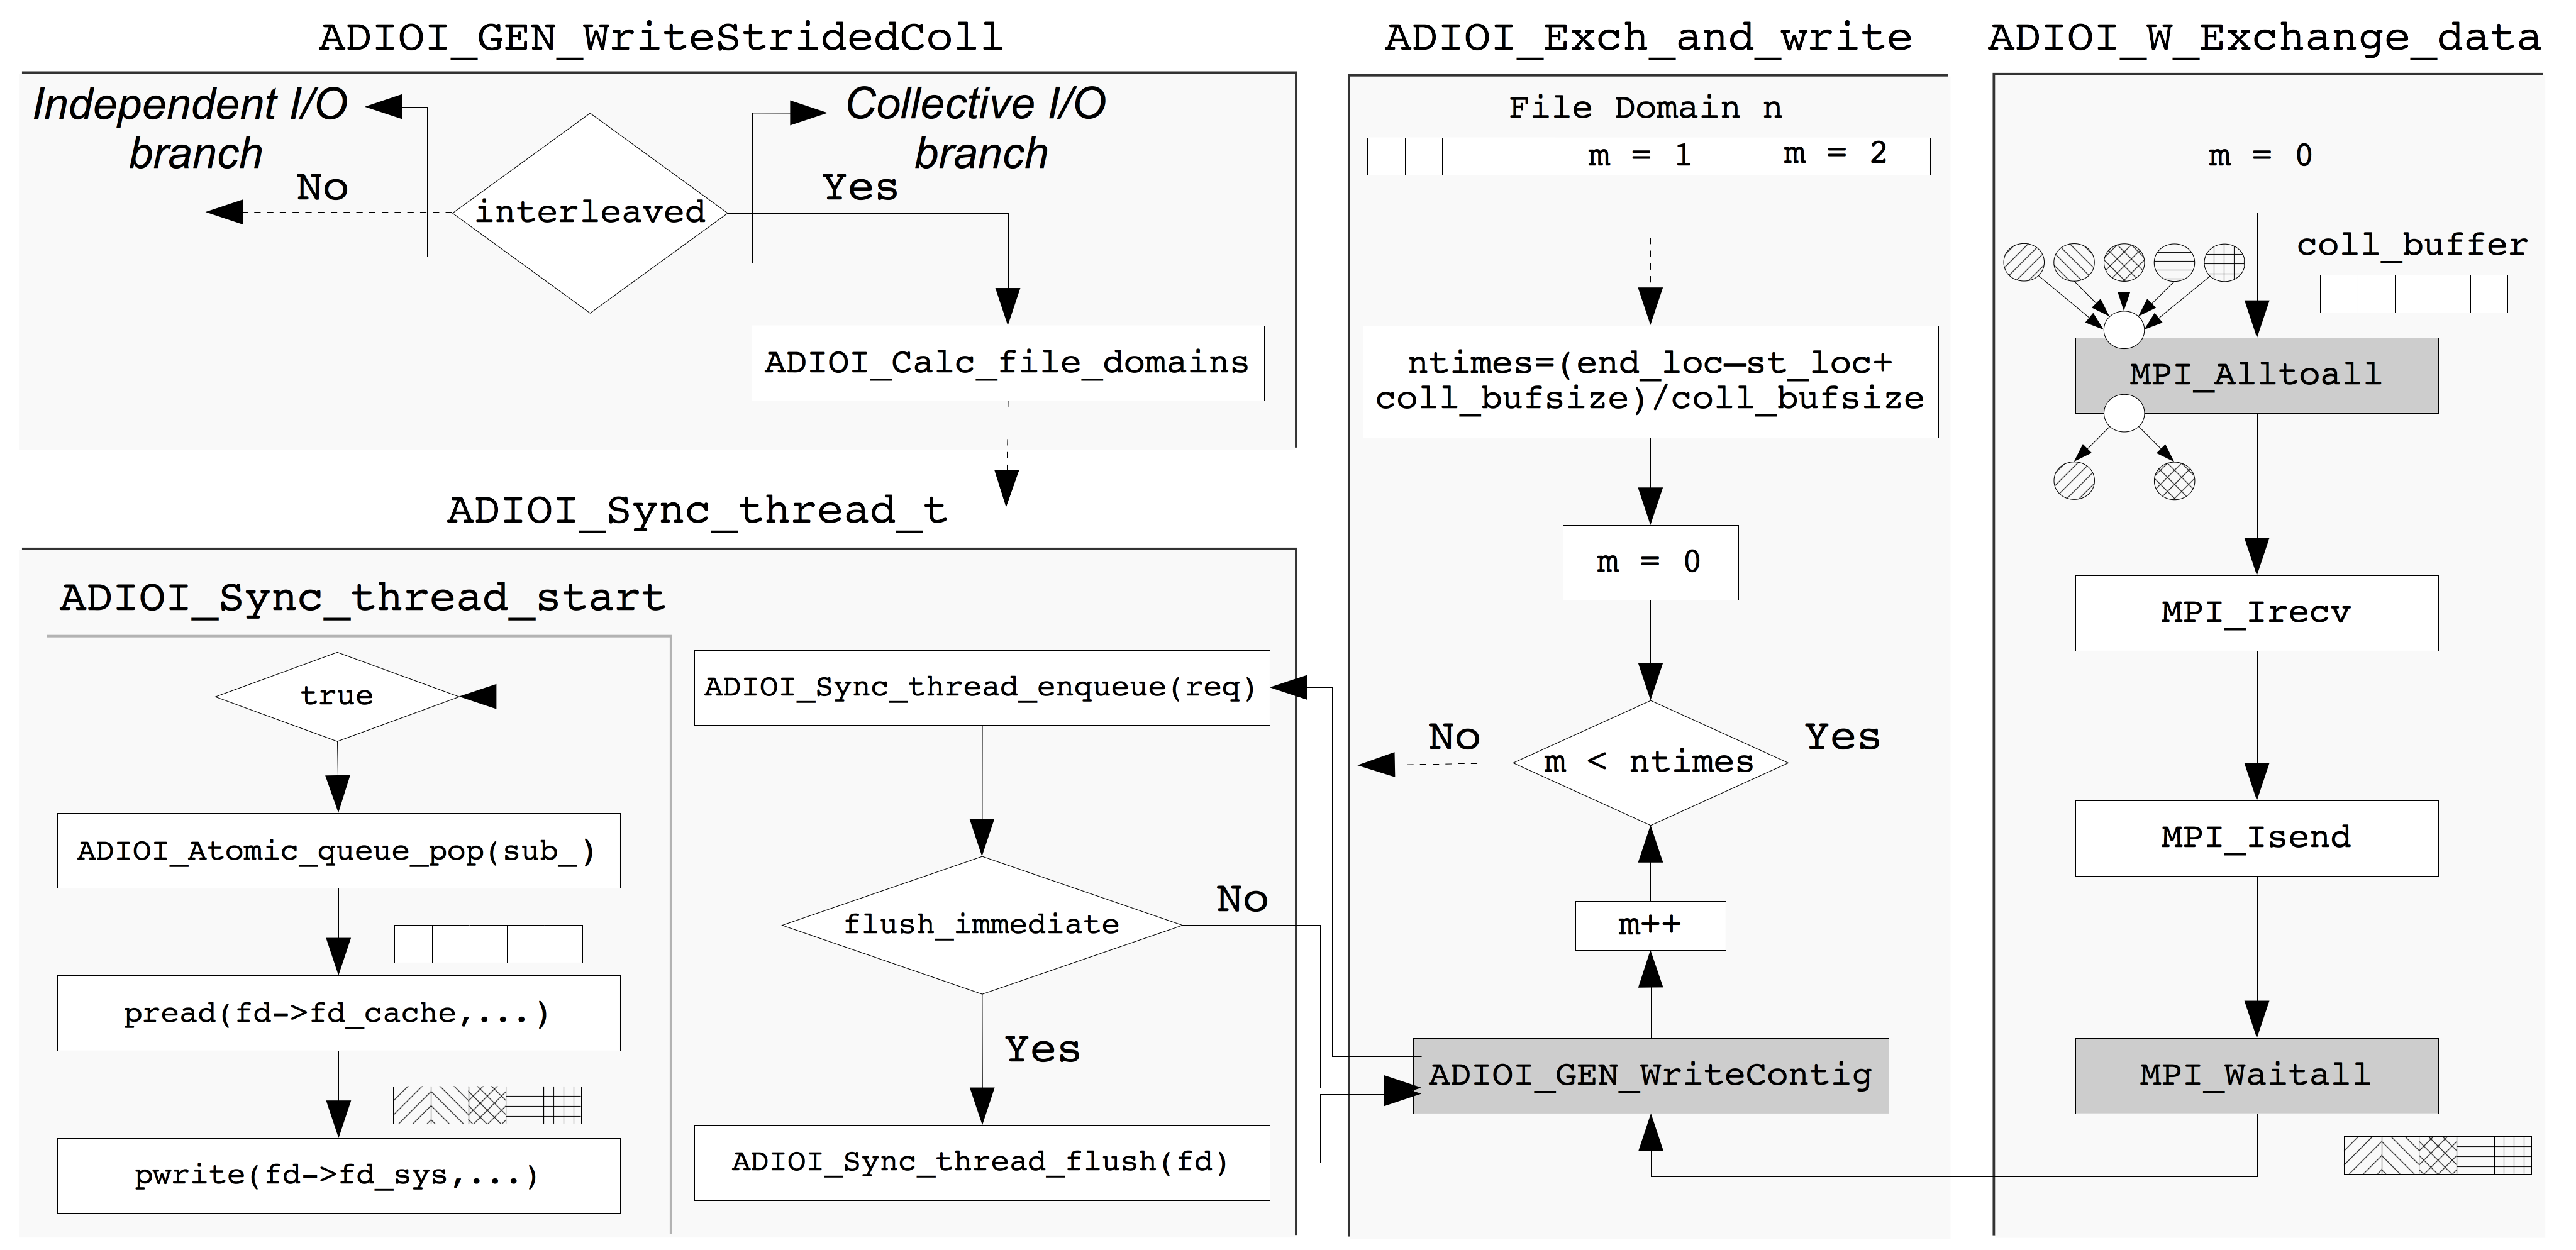
\includegraphics[angle=90,width=0.8\textwidth]{figures/ext2ph+e10_t}
  \caption{Extended collective I/O flow diagram including cache plugin support.}
  \label{figure: coll_io_cache}
\end{figure}
The first part of the diagram in the upper left part is left unchanged. The changes are introduced in the \codeword{ADIO\_GEN\_WriteContig()}\footnote{In the BeeGFS driver this is replaced by 
\codeword{ADIOI\_BEEGFS\_WriteContig()}.} operation. This has been modified to redirect writes to the local file system cache whenever the cache is enabled, that is, when the \codeword{e10\_cache} 
hint is set to enable. After data is written to the cache, the function creates a new synchronization request of type \codeword{ADIOI\_THREAD\_SYNC} by invoking \codeword{ADIOI\_Sync\_req\_init()} 
and enqueues it into the pending queue of the synchronization thread through \codeword{ADIOI\_Sync\_thread\_enqueue()}. At this point the main thread also checks the desired flushing policy defined by 
the \codeword{e10\_cache\_flush\_flag} hint. If the hint is set to \codeword{flush\_immediate} the main thread immediately flushes the enqueued requests to the submission queue by invoking 
\codeword{ADIOI\_Sync\_thread\_flush()} and then returns. Otherwise requests are left in the pending queue and will be served when the file is closed with \codeword{MPI\_File\_close()} or when the 
main thread invokes \codeword{MPI\_File\_sync()}.

\subsection{BeeGFS Cache Integration in ROMIO}
The BeeGFS file system provides its own caching infrastructure, which includes a set of APIs to control the caching functionalities and a daemon process, running on the host machine, that takes care of 
moving data between the cache and the global file system. For this reason, some of the cache plugin features presented before for the universal file system module in the common layer are redundant. In 
particular, we do not any longer need to manually open a cache file in the host and start a pool of synchronization threads. When using the BeeGFS cache API the file system takes care of all these aspects 
for us. Nevertheless, we still reused some parts of the cache plugin to integrate the BeeGFS cache support into ROMIO. For more details about the cache implementation in the BeeGFS driver refer to the
source code at http://www.github.com/gcongiu/E10.git.

\subsection{Consistency Semantics}
As far as write consistency semantic is concerned, the MPI-IO interface does not make any assumption regarding the underlying parallel file system or its semantics. ROMIO specifically supports file systems that are 
both POSIX compliant, like Lustre, and non-POSIX compliant, like NFS or PVFS. In MPI-IO, written data becomes globally visible only after either \codeword{MPI\_File\_sync()} or \codeword{MPI\_File\_close()} 
are invoked on the MPI file handle and by default there is no write atomicity. The motivation is that data can be cached at some level locally in the compute nodes. The ROMIO implementation can overcome the 
risk of data inconsistency, e.g., related to false sharing of file system blocks, using persistent file realms~\cite{ColomaCWWRP04}, and can even enforce atomicity using \codeword{MPI\_File\_set\_atomicity()}.

In our implementation we comply to the MPI-IO semantics just described. This means that data written to the local file system cache using the newly introduced MPI-IO hints will be globally visible to the rest 
of the nodes only under the following circumstances:

\begin{itemize}
\item The \codeword{e10\_cache\_flush\_flag} has been set to \codeword{flush\_immediate} by the user and synchronization, started automatically by the implementation right after the write operation, has completed;
\item The \codeword{e10\_cache\_flush\_flag} has been set to \codeword{flush\_onclose} by the user and the invoked \codeword{MPI\_File\_close()} has returned;
\item The \codeword{MPI\_File\_sync()} function has been invoked by the user and it has returned.
\end{itemize}

Consistency for reading data from the cache is not clearly defined by the ext2ph algorithm. In general, data written to the local file system cache can be read back from the user without accessing the global 
file system. However, the algorithm calculates the location of a data block based on the number of aggregators, their logical position within the set of aggregators, and the size of the complete data set. 
This means that a collective read that matches the previous write could safely retrieve the data from the aggregators' cache without incurring into any problem. In spite of that, in general reading from the 
cache requires additional metadata describing the file layout across the caches. For this reason, we currently do not support reads from the local file system cache.

Furthermore, whenever required, we can enforce cache coherency ensuring that read operations cannot access data that is currently in transit, i.e., not or only partially moved from the cache to the global file. 
This can be done by locking the file domain extent being cached until all the data has been made persistent in the global file. For this purpose ROMIO provides a set of internal locking macros, namely 
\codeword{ADIOI\_WRITE\_LOCK}, \codeword{ADIOI\_READ\_LOCK} and \codeword{ADIOI\_UNLOCK} that we used in our implementation. The lock of cached data can be selected by setting the \codeword{e10\_cache} hint in 
Table~\ref{table: hints_table} to \codeword{coherent}. This will \codeword{enable} the cache and set locks appropriately, assuming underlying file system support.

\subsection{Changes to the Application's Workflow}
Simplifying, most HPC simulation codes can be divided into multiple phases of computation, in which data is produced, and I/O, in which data is written to persistent storage for post-processing purposes as well as 
defensive checkpoint/restart. Focusing on the I/O phase and considering the case of applications writing to a shared file, the I/O phase can be divided into the following steps:

\begin{enumerate}
\item The file is opened using \codeword{MPI\_File\_open()}: at this point the info object containing the user defined MPI-IO hints is passed to the underlying ROMIO layers;
\item Data is written to the file using \codeword{MPI\_File\_write\_all()}: this function invokes the underlying \codeword{ADIOI\_GEN\_WriteStridedColl()} previously described in Figure~\ref{figure: coll_io_impl};
\item The file is closed using \codeword{MPI\_File\_close()}: after the file is closed data must be visible to every process in the cluster. 
\end{enumerate}

To take advantage of the proposed MPI-IO hint extensions, the application's workflow has to be modified. Figure~\ref{figure: workflow} shows the classical application's workflow (cache disabled) as well as the modified 
version using the new hints (cache enabled). The difference is that, in order to take advantage of the proposed hints and hide the cache synchronization to the computation phase, the \codeword{MPI\_File\_close()} for the 
I/O phase \textit{k} has been moved at the beginning of the I/O phase \textit{k+1}, just before the new file is opened.

\begin{figure}[!htb]
  \centering
  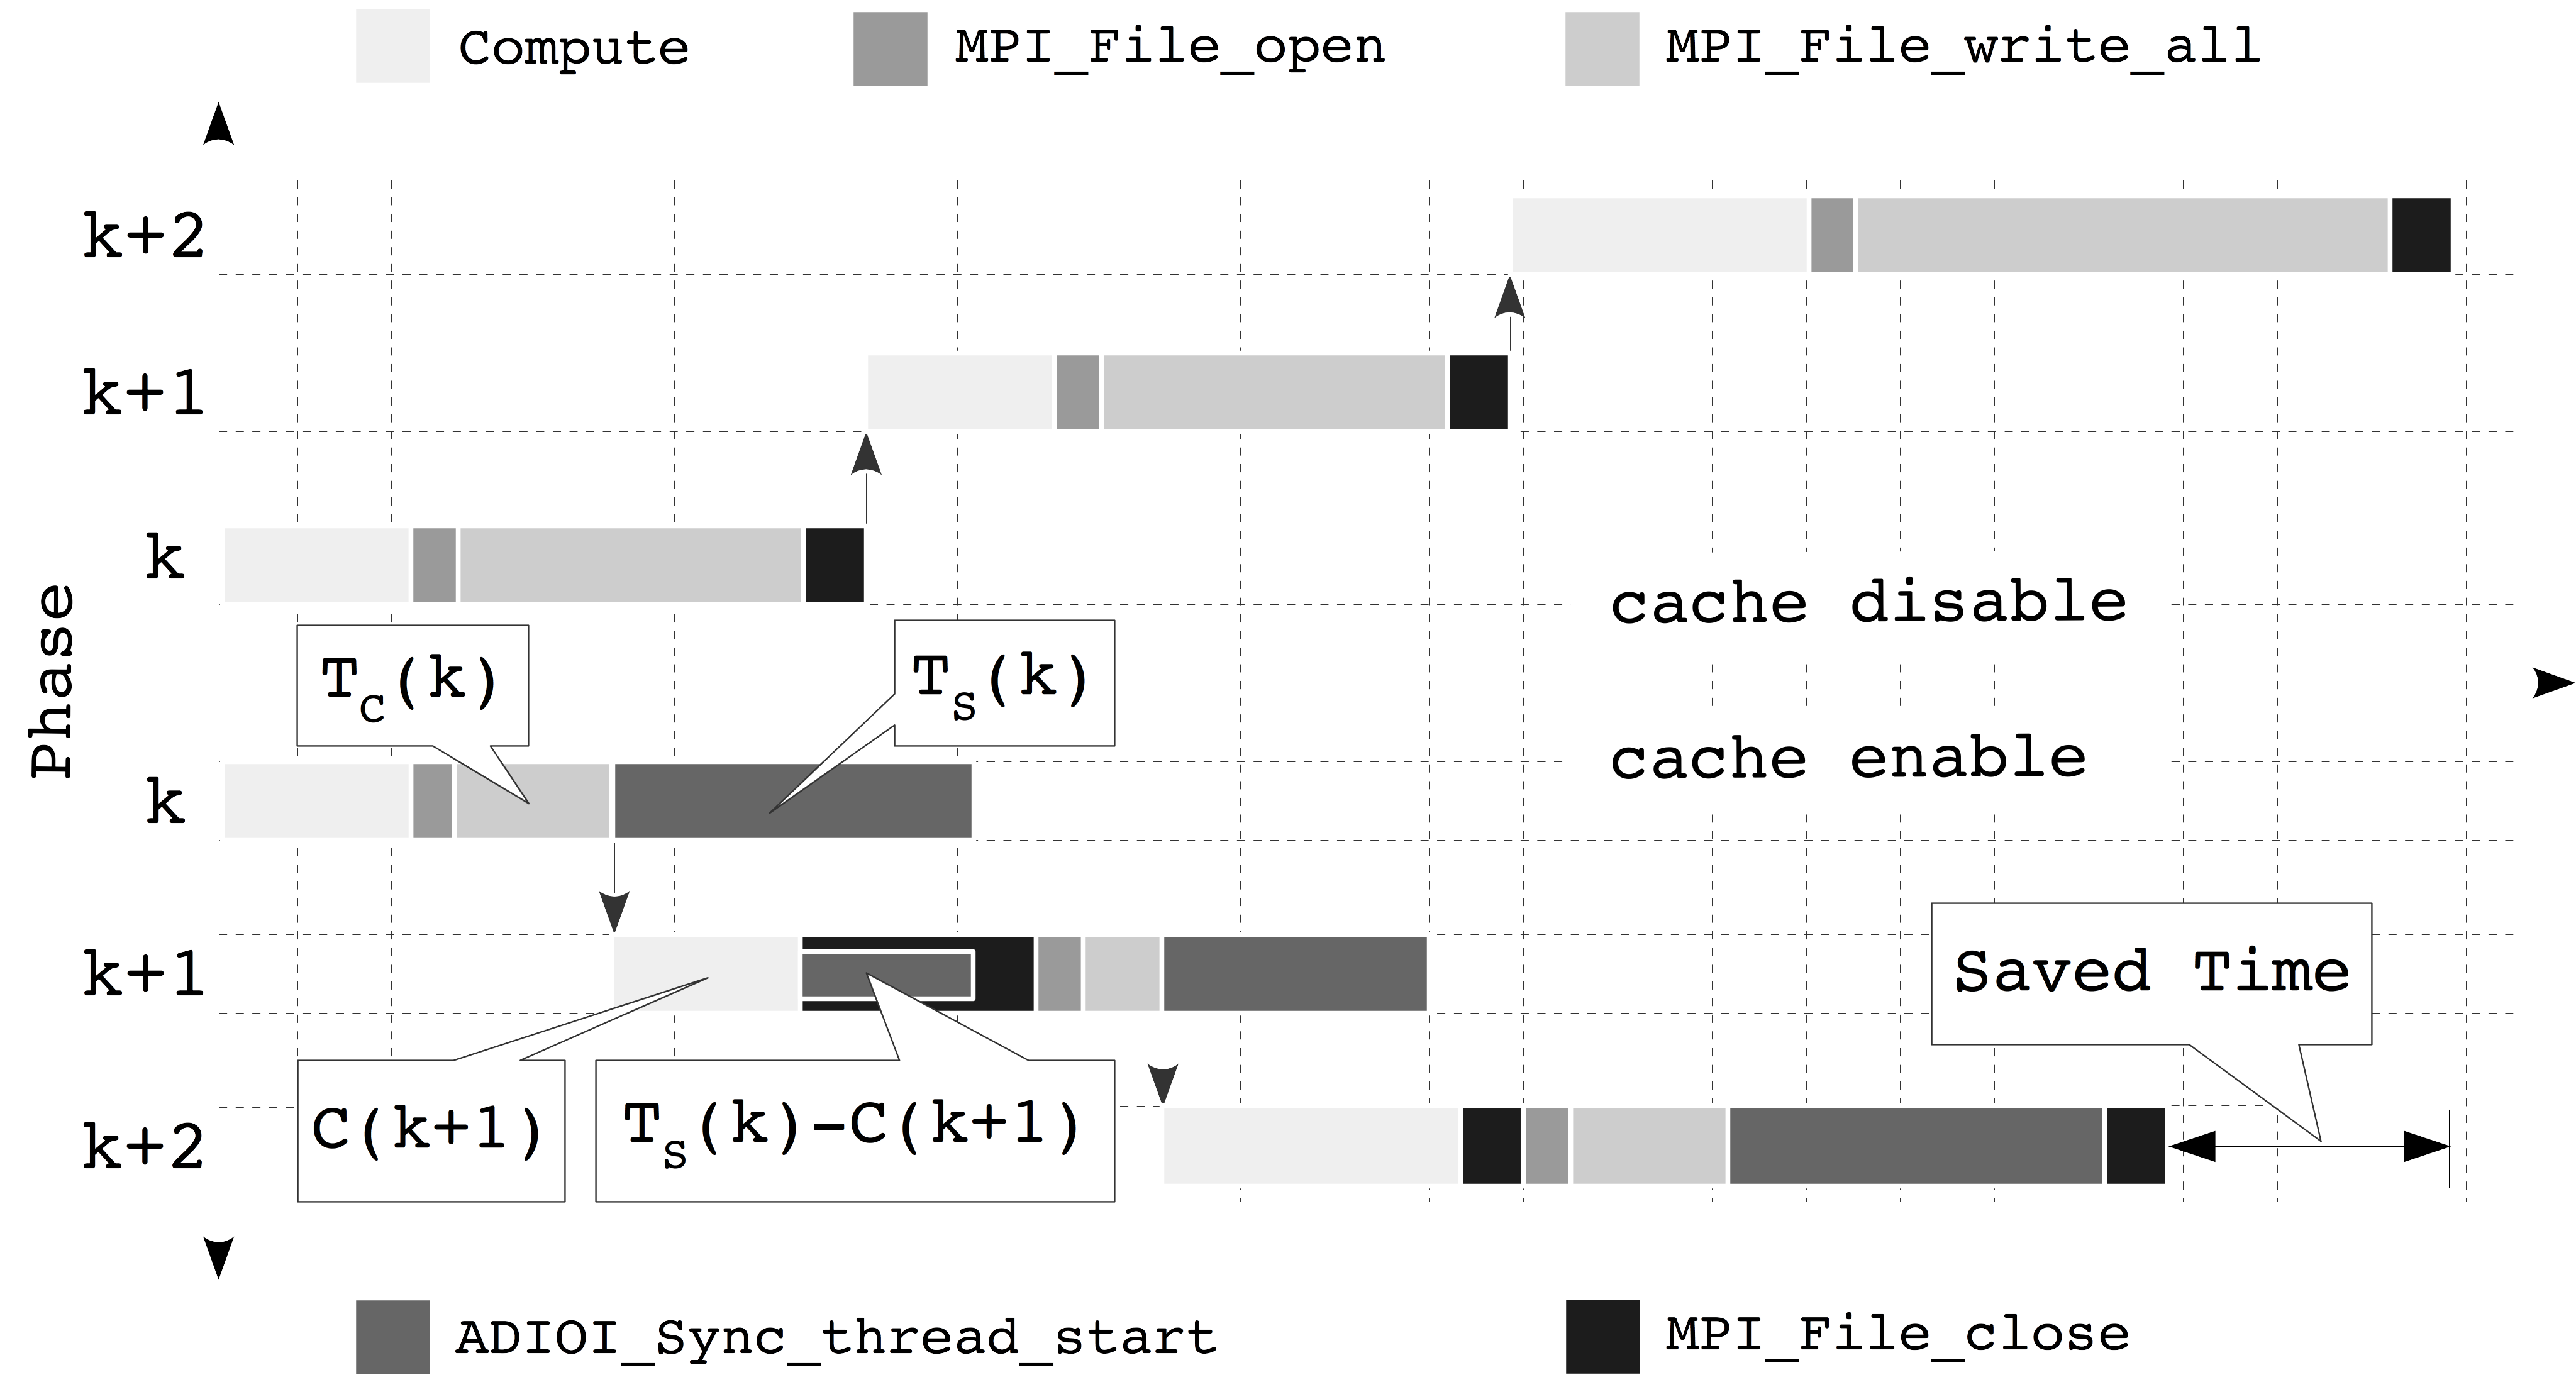
\includegraphics[width=0.9\textwidth]{figures/workflow_baw}
  \caption{Standard and modified workflows. When cache is disabled compute phase `k+1' starts after file `k' has been closed. 
  When the cache is enabled compute `k+1' can start immediately after data has been written. At the same time, background 
  synchronization of cached data starts. File `k' is closed before the file `k+1' is opened, forcing the implementation to wait 
  for cache synchronization to complete.}
  \label{figure: workflow}
\end{figure}

\subsubsection{MPIWRAP Library}
Since the workflow modification just presented might not be feasible for legacy applications, we developed a MPI-IO wrapper library (called MPIWRAP), written in C++, that can reproduce this change behind the scenes. 
The library can be linked to the application or preloaded with \codeword{LD\_PRELOAD} and has been used for all the experiments contained in this thesis. MPI-IO hints are defined in a configuration file and passed 
by the library to \codeword{MPI\_File\_open()}. We can define multiple hints targeting different files or groups of files. The library overloads \codeword{MPI\_\{Init,Finalize\}()} and \codeword{MPI\_File\_\{open,close\}()} 
using the PMPI profiling interface. The workflow modification can be triggered for a specific set of files (identified by the same base name) in the configuration file. Whenever one of such files is closed, our \codeword{MPI\_File\_close()} 
implementation will return success. However, the file will not be really closed. Instead, its handle will be kept internally for future references. When the next shared file with the same base name is opened, our 
\codeword{MPI\_File\_open()} implementation will search for outstanding opened file handles and will invoke \codeword{PMPI\_File\_close()} on them before opening the new file, thus triggering the cache synchronization 
completion check for each of them.

\subsection{Write Bandwidth}
According to the new I/O workflow, described in this section, we have that being $S(k)$ the amount of data written during phase \textit{k}, $T_c(k)$ the time needed to write $S(k)$ collectively to the cache using 
\codeword{MPI\_File\_write\_all()}, $T_s(k)$ the time needed to synchronise the cached data in every aggregator to the global file system (through \codeword{ADIOI\_Sync\_thread\_start()}), and $C(k+1)$ the 
computation time of phase \textit{k+1}, the resulting write bandwidth for \textit{k} is expressed by Equation~\ref{formula: bw}:

\begin{equation}\label{formula: bw}
        bw(k) = \frac{S(k)}{T_c(k) + max(0,\ T_s(k) - C(k+1))}
\end{equation}
Therefore, the total average bandwidth perceived by the application is:
\begin{equation}\label{formula: abw}
        BW = \frac{\sum_{k=0}^{N-1} S(k)}{\sum_{k=0}^{N-1} T_c(k) + max(0,\ T_s(k) - C(k+1))}
\end{equation}

From Equation~\ref{formula: bw} (in which we have considered the open time neglectable) it is clear that the maximum performance can be obtained when $C(k+1) \geq T_s(k)$, that is, when we can completely hide 
cache synchronization to the computation phase. On the other hand when $C(k+1) < T_s(k)$ we might have a minima in the bandwidth since \codeword{MPI\_File\_close()} needs to wait for cache synchronization 
completion (Figure~\ref{figure: workflow}). 

\section{Contributions} \label{sec: nvm-related}
Many research works have tried to optimize collective I/O focusing on different aspects. Yu and Vetter~\cite{Yu08} before us have identified the global synchronization 
problem as one of the most severe for collective I/O performance. They exploited access pattern characteristics, common in certain scientific workloads, to partition collective 
I/O into smaller communication groups and synchronise only within these. Block-tridiagonal patterns, not directly exploitable, are automatically reduced, through an intermediate 
file view, to a more manageable pattern and can thus take advantage of the proposed solution. The ADIOS library~\cite{Lofstead2008} addresses this problem similarly by dividing a 
single big file into multiple files to which collective I/O is carried out independently for separated smaller groups of processes. 

Lu et al.~\cite{Lu2012}~\cite{Lu2013} further explored collective I/O performance beyond global synchronization and considered memory pressure of collective I/O buffers. They proposed 
a memory conscious implementation that accounts for reduced memory per core in future large scale systems. Liao~\cite{Liao11} focused on the file domain partitioning impact on parallel 
file systems' performance. He demonstrated that by choosing the right file domain partitioning strategy, matching the file system locking protocol, collective write performance can be 
greatly improved.

Chen et al.~\cite{Chen2011} addressed the problem of I/O server contention using a layout aware strategy to reorganize data in aggregators. On the same lines, 
Xuechen et al.~\cite{Zhang2009} proposed a strategy to make collective I/O `resonant' by matching memory layout and physical placement of data in I/O servers and exploiting 
non-contiguous access primitives of PVFS. The strategy proposed is similar in concept to the Lustre implementation of collective I/O in which file contiguous patterns are converted to 
stripe contiguous patterns and the concurrency level on OSTs can be set using the MPI-IO hint \codeword{romio\_lustre\_co\_ratio} (Client-OST ratio). 

Liu et al.~\cite{Liu2013} exploited the scheduling capabilities of PVFS I/O servers to rearrange I/O requests' order and better overlap read and shuffle phases among different processes. 
Yu et al.~\cite{Yu2007} used the file joining functionalities of Lustre to convert collective I/O into independent I/O to multiple files, thus avoiding file system stripe contention. All 
resulting files are afterwards rejoined into a single shared file.

Lee et al.~\cite{LeeRTXW04} proposed RTS as infrastructure for remote file access and staging using MPI-IO. Similarly to our approach, RTS uses additional threads, 
Active Buffering Threads (ABT)~\cite{XiaosongWLS03}, to transfer data in background to the compute phase. Moreover, the authors also modified the ABT ROMIO driver implementation to stage data in 
the local file system whenever the amount of main memory runs low. Although they include collective I/O in their study, they lack a detailed evaluation of the impact that SSD caching can have on 
the different performance contributions of collective I/O and the additional reduction of memory pressure. Furthermore, remote staging of data requires additional nodes while we collocate storage 
with compute. The SCR library~\cite{Moody2010}~\cite{Moody2010_2} also uses local storage resources to efficiently write checkpoint/restart data but this is targeted to a specific use case and requires the modification of 
the application's source code to be integrated. 

Other works, focus on I/O jitter reduction using multi-threading and local buffering resources~\cite{DorierACSO12}, but we do an evaluation of collective I/O and show how the effect of I/O jitter can 
become even more prominent when using fast NVM devices. More recently the Fast Forward I/O project~\cite{Lofstead2016}, from U.S. Department of Energy (DOE), proposed a burst buffer architecture to absorb 
I/O bursts from file system clients into a small number of high performance storage proxies equipped with high-end solid state drives. This technique has been, e.g., implemented in the DDN Infinite Memory 
Engine\footnote{\url{http://www.ddn.com/products/infinite-memory-engine-ime14k}}. Even though the burst buffer solution is interesting, it may require very expensive dedicated servers as well as significant 
changes to the storage system architecture. 

Unlike previous works, we proposed a fully integrated, prototype solution for new available memory technologies able to scale aggregate bandwidth in collective I/O with the number of available compute 
nodes. Additionally, our solution does not require any proprietary hardware or dedicated kit to work. We demonstrate that SSD based cache can reduce the synchronization overhead intrinsic in the collective 
I/O implementation in ROMIO as well as the requirement for large collective buffers (memory pressure). Our implementation is compatible with legacy codes, since it does not require any change at the application 
level, and can work out of the box with any backend file system, although in DEEP-ER we focused on BeeGFS. At the moment the cache synchronization is implemented in the ADIO UFS driver using pthreads. 
Future releases of BeeGFS will support native caching, including asynchronous flushing of local files to global file system. We have already integrated ROMIO with a BeeGFS driver that will take advantage of 
these functionalities.

\chapter{Evaluation} \label{chapt: evaluation}
In this chapter we present results for the Mercury middleware and the MPI-IO hints extensions for collective I/O proposed in previous chapters. For Mercury we consider a high energy physics code.
This application is representative of a class of HPC analysis applications that are becoming more and more common in workloads of leadership class systems. Our goal is to demonstrate that through
user guided I/O prefetching even a non-optimized application can improve its I/O utilization (and thus performance) of the file system.
For our ROMIO improvements we consider a range of collective I/O benchmarks that include synthetic and real application kernels. We run every benchmark with the baseline collective I/O implementation
in ROMIO and discuss in detail all the ext2ph performance implications; then we enable our NVM based optimization and show how the same performance implications can be mitigated or completely
cancelled when taking the global parallel file system out of the ext2ph critical I/O path.

\section{I/O Prefetching in ROOT}
Our target real world application is written using `ROOT', an object-oriented framework widely adopted in the experimental high energy physics community to build software 
for data analysis. The application runs on the Mogon cluster at the data processing center of the University of Mainz (ZDV), in Germany. It analyzes particle data read from 
an input file structure using the `ROOT' format (structured file format).

\begin{figure*}[!htb]
  \centering
  \begin{subfigure}[t]{0.7\textwidth}
    \centering
    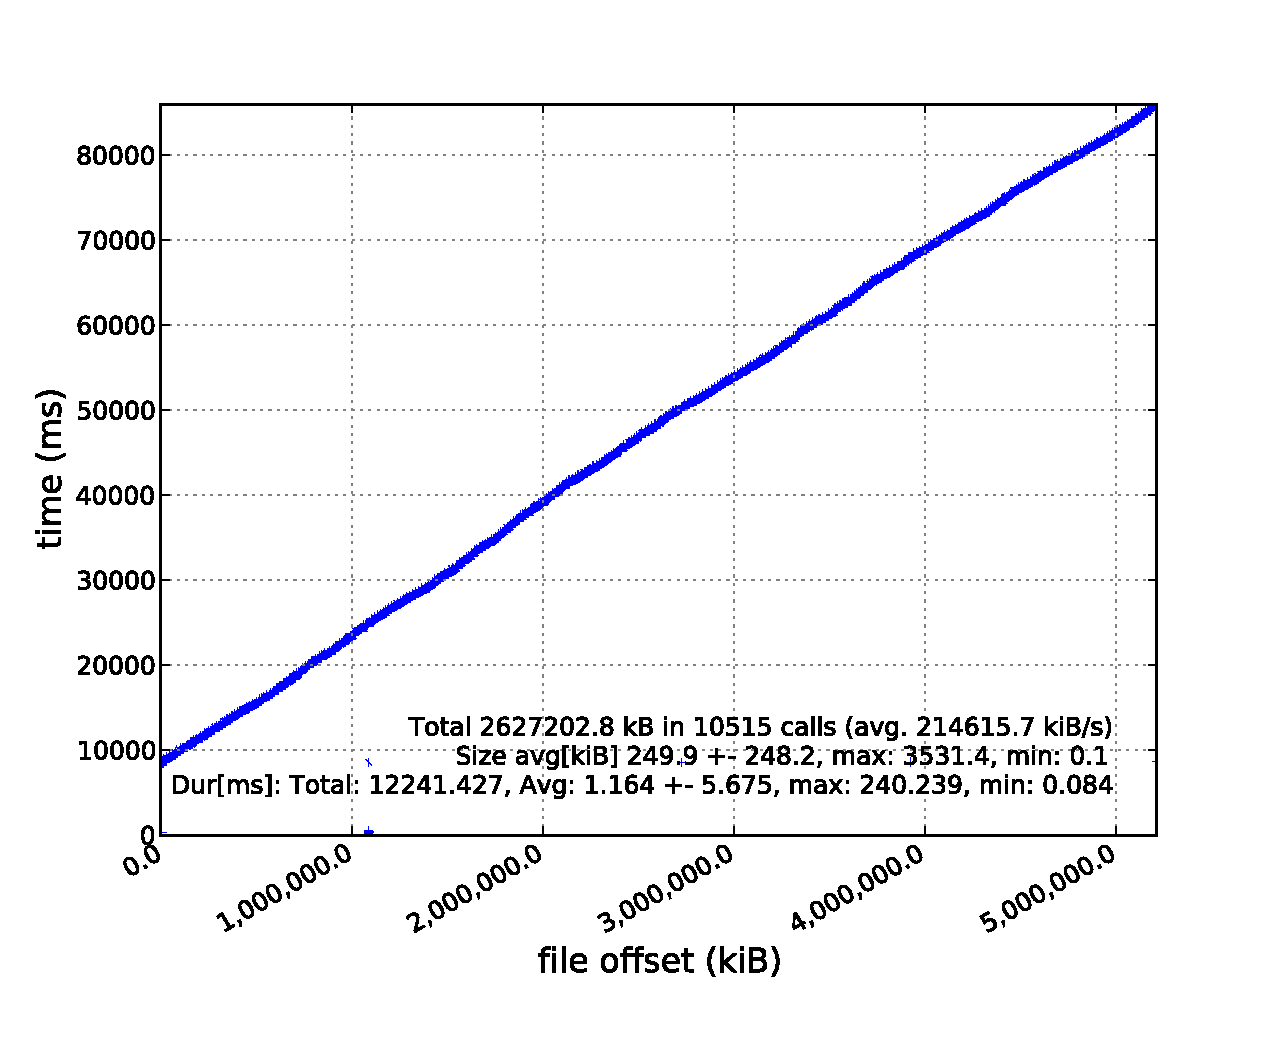
\includegraphics[width=\textwidth]{figures/iopat_profile}
    \caption{\textit{}}
    \label{figure: iopat_profile}
  \end{subfigure}
  \begin{subfigure}[t]{0.7\textwidth}
    \centering
    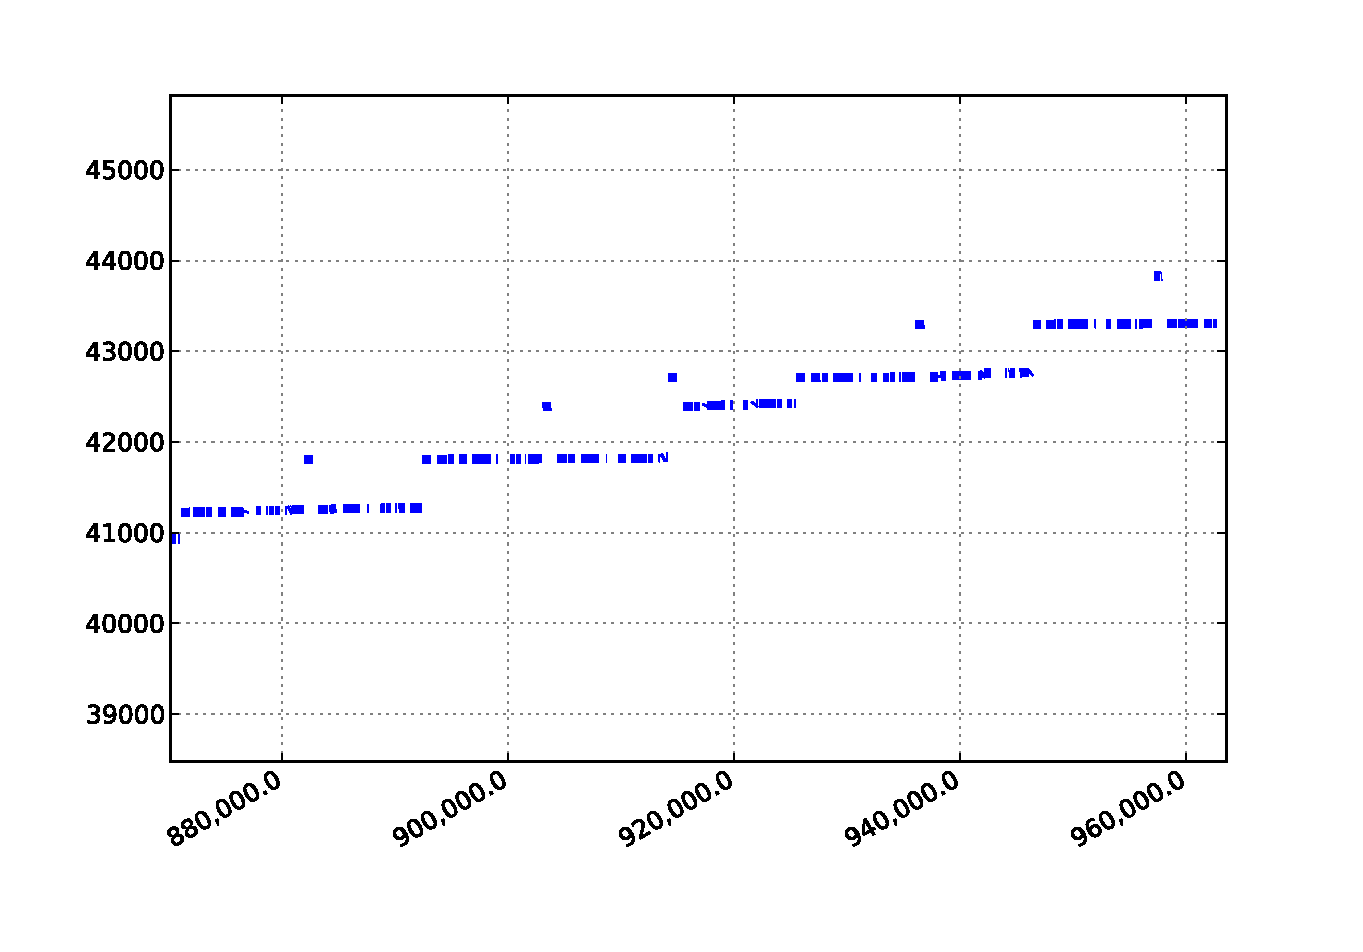
\includegraphics[width=\textwidth]{figures/00050_zoom}
    \caption{\textit{}}
    \label{figure: iopat_zoom}
  \end{subfigure}
  \caption{I/O read profile of the target application under analysis (\ref{figure: iopat_profile}), extracted from the the GPFS file system in the test cluster, and zoomed 
  window (\ref{figure: iopat_zoom}) showing the actual pattern details.}
  \label{figure: iopattern_with_statistics}
\end{figure*}

First of all we characterized the application's I/O pattern for a target file using traces and statistics extracted through several tools such as \textit{strace}, \textit{ioapps}\footnote{\url{https://code.google.com/p/ioapps}.} 
and GPFS's \textit{mmpmon} monitoring tool. 
Figure~\ref{figure: iopattern_with_statistics} shows the I/O pattern along with some additional statistics. As it can be seen, in this specific case (5 GB file), the application issues a total of 
10515 \texttt{read()} system calls to read about 2.6 GB of total data. The average request size is 250 KB and the time spent waiting for I/O is 12 seconds, when running on the test cluster. 

At a first glance the general I/O behaviour of the application looks sequential, most of the accesses to the file follow an increasing offset. Nevertheless, adjacent reads are separated by gaps 
(a strided read pattern). In a few cases this gap becomes negative, meaning that the application is moving backwards in the file to read some data previously left behind (as reported in 
Figure~\ref{figure: iopat_zoom}).

After a detailed I/O pattern analysis we could divide the target file into contiguous non-overlapping ranges. Within these ranges reads happen to have increasing offset. Even though the general 
I/O pattern of the application for different files looks similar\footnote{Due to space limits we do not report the comparison between different files.}, the size of the non-overlapping ranges may 
change significantly. This general behaviour can be modelled using Mercury through a configuration file in which a `WillNeed' hint covers the whole file from beginning to end (i.e., `Offset' and `Length' equal to 
0). The backwards seeks can be accounted for using the `CacheSize' parameter to keep previously accessed blocks in cache. In this way we effectively emulate a sliding window that tracks the application's 
I/O behaviour. This would not be possible by just using a, e.g., \texttt{POSIX\_FADV\_WILLNEED} advice on the whole file before starting the application like shown by Figure~\ref{figure: fadvise_comparison}. 
The reason is that even if the file fits entirely into the cache, we would have a large number of valuable pages, possibly from other applications, discarded from the cache to load data that will be accessed at the end of 
the application. Additionally, if the file size is bigger than the cache size we would have the file system discarding blocks at the beginning of the file as the blocks at the end are preloaded, 
effectively forcing the application to access these blocks from the I/O servers instead of the cache. With our approach, on the other hand, we keep in the cache only a small, controlled number of 
blocks (the ones currently accessed), while the older blocks are discarded since no longer needed.

\begin{figure}[!htb]
  \centering
  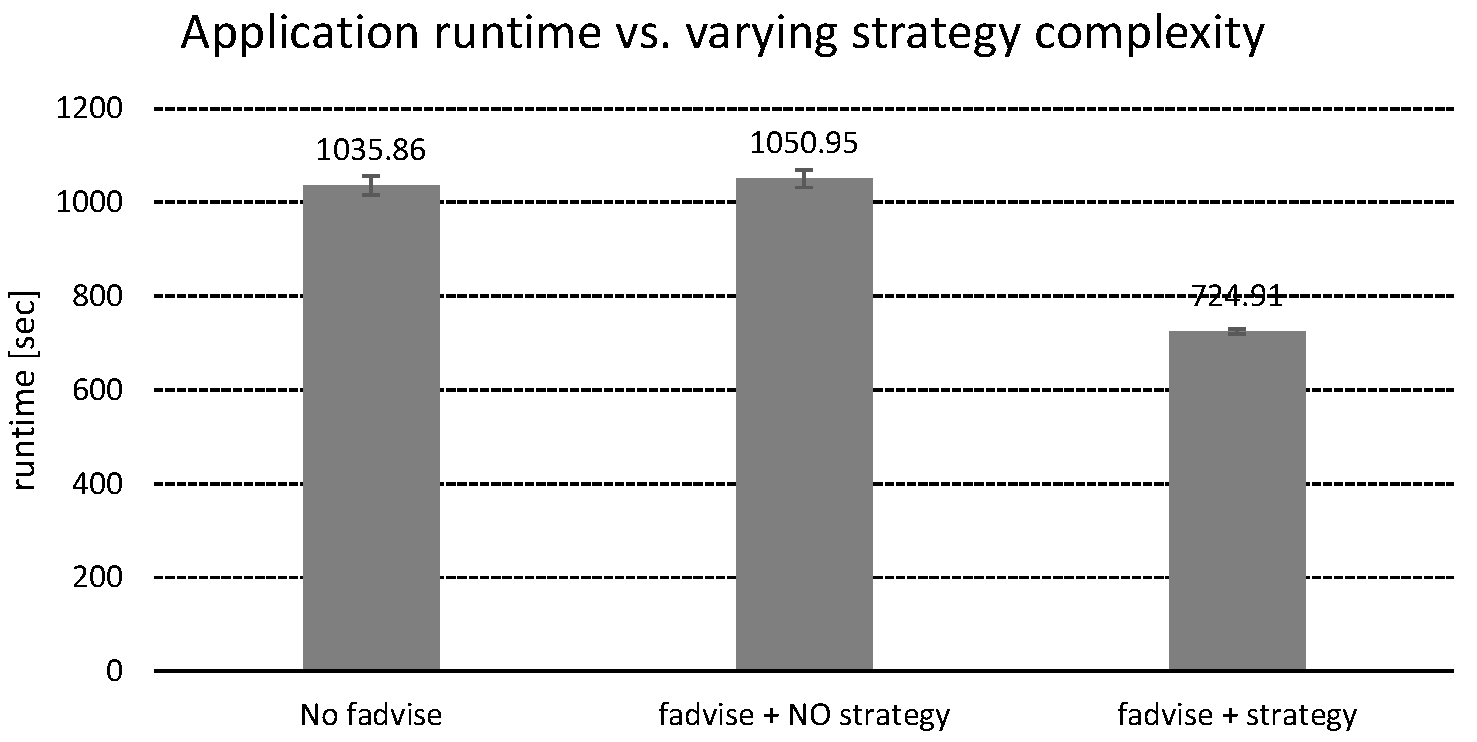
\includegraphics[width=0.8\textwidth]{figures/test_fadvise_no_border}
  \caption{Comparison between different usage stategies of posix\_fadvise for an input file of 55 GB residing in an ext4 file system. The first bar represents the case in which no advice is used, 
  the second bar represents the case in which a POSIX\_FADV\_WILLNEED is issued for the whole file at the beginning of the application and the third bar represents the case in which POSIX\_FADV\_WILLNEED 
  is issued using Mercury.}
  \label{figure: fadvise_comparison}
\end{figure} 

To assess the impact of our Mercury prototype on the application and file systems performance we considered the application execution time and the number of reads accounted for by the respective file systems. 
We conducted our experiments without file system hints and then with file system hints issued transparently to the application by the \textit{Advice Manager}. Furthermore, we ran each experiment three 
times and calculated average, minima and maxima for each metric. In order to avoid caching affecting our measurements, extra care was taken to clean all the relevant caches for the different file systems. 
For ext4 and Lustre this was accomplished by using the command line: $$echo\ 3 > /proc/sys/vm/drop\_caches$$ on the file system clients. Additionally, for Lustre this command was also executed on the
\textit{object storage servers} (OSSs) to avoid the server side cache to be retained. In the case of GPFS, the file system client's page pool was cleaned using the clean file cache hint in Table~\ref{table: hints_table}, 
the GPFS \textit{network shared disks} (NSDs)\footnote{GPFS name for I/O servers.} servers do not cache any data. 


\subsection{Testbed}
Our testbed is composed by a test cluster of seven nodes, mainly intended to evaluate the proposed Linux kernel modifications with the Lustre file system. The reason 
for using a smaller cluster instead of the Mogon system is that it was not possible to disrupt the production cluster, affecting hundreds of users, by re-installing 
the operating system kernel. In order to make realistic comparisons between Lustre and GPFS, the test cluster also has a GPFS file system on comparable hardware. 

Both file systems have a single disk server each, one Dell R710 acts as GPFS network shared disk (NSD) server and another as Lustre object storage server. The R710 are equipped 
with two quadcore E5620 @2.4 GHz and 24 GB main memory. For storage, both disk servers share a MD3200 array with 2 controllers and 4 MD1200 expansion shelves for a total 
of 60 2 TB drives. The Storage is formatted in 4 15 dynamic disk pools. This is the LSI/Netapp type of declustered RAID, which distributes the 8+2 RAID6 stripes evenly 
over all 15 disks for better rebuild performance. The disk block size is set to 128 KB, which results in a RAID stripe size of 1 MB. The four disk pools are then split 
on the Array into LUNs, one of the LUNs from each disk pool is then used for GPFS and another one from each pool is used for Lustre. This results in comparable resources 
for both file systems and tests do not interfere with each other, as long as only one file system is tested at a time. 

While the GPFS filesystem embeds the metadata with the data, Lustre needs a separate Metadata Server (MDS). This is hosted by a SuperMicro server equipped with one quadcore Xeon 
E3-1230 @3.3 GHz and 16 GB of main memory, as metadata target (MDT) it uses a 120 GB SSD Intel 520. Four other machines of the same type, equipped with an eight core E3-1230 @3.3 
GHz processor and 16 GB of main memory, work as compute nodes and file system clients. All machines, servers and clients, are equipped with Intel X520DA 10 Gigabit adapters and 
connected to a SuperMicro SSE-X24S 24 ports 10 Gigabit switch. Both, the GPFS and Lustre file systems are formatted with a block size of 4 MB.

\subsection{Performance Results}
To measure the performance improvements that our Mercury prototype can deliver to the application's run-time we conducted two set of tests. In the first test we varied the size of the input file from 5 to 95 GB. 
This is mainly aimed to study the behaviour of the `ROOT' application using different input file sizes and how our solution behaves when the file becomes bigger than the available cache space. In the second 
test we varied the number of `ROOT' instances running simultaneously from 1 to 8. By doing so we study the interaction of multiple processes accessing the file system and how these can benefit from the prefetching 
hints generated by Mercury. Figures~\ref{figure: run-time_1} and~\ref{figure: run-time_2} report the results for the described experiments. All the tests where performed using a `BlockSize' of 4 MB, a `CacheSize' of 
8 blocks, a `ReadAheadSize' of 4 blocks, and a `WillNeed' hint covering the whole file (i.e., with `Offset' and `Length' equal to 0), resulting in each process consuming up to 32 MB of cache space and 512 MB in total 
for 8 application instances. 

The `WillNeed' on the whole file causes the \textit{Advisor Thread} to issue up to 4 (`ReadAheadSize') prefetching requests for blocks of 4 MB sequentially, starting from the current accessed 
block. This has the same effect of data sieving in ROMIO, optimizing the access size and allowing the application to read the requested data randomly from the cache instead of the file system. The produced effect is 
particularly beneficial in the case of Lustre and ext4, as it can be seen in Figures~\ref{figure: ext4_1} and~\ref{figure: lustre_1}. In these cases we measure reductions in the execution time of up to 50\%, with respect 
to the normal case. For GPFS we can still observe an improvement, but this is more contained compared to the other file systems (Figure~\ref{figure: gpfs_1}). The reductions in the execution time measured in GPFS are on 
average up to 10\%, with respect to the normal case. The reason is that the default prefetching strategy in GPFS works better that traditional read-ahead. In fact, by disabling the prefetching in GPFS we observed reductions 
in the execution time comparable to the other file systems (not reported here).

%\begin{figure}[!htb]
%  \centering
%  \begin{subfigure}[t]{0.48\textwidth}
%    \centering
%    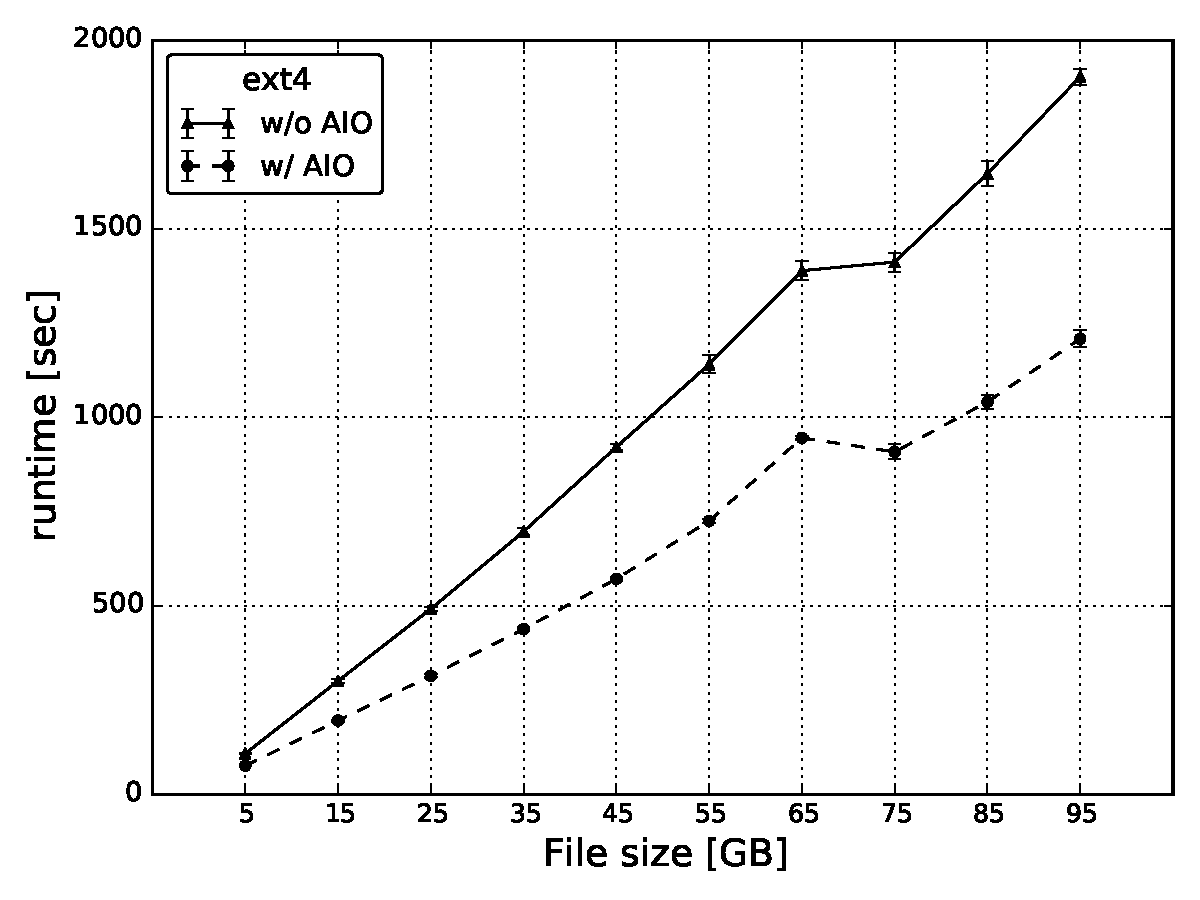
\includegraphics[width=\textwidth]{figures/ext4/runtime}
%    \caption{\textit{}}
%    \label{figure: ext4_1}
%  \end{subfigure}
%  \begin{subfigure}[t]{0.48\textwidth}
%    \centering
%    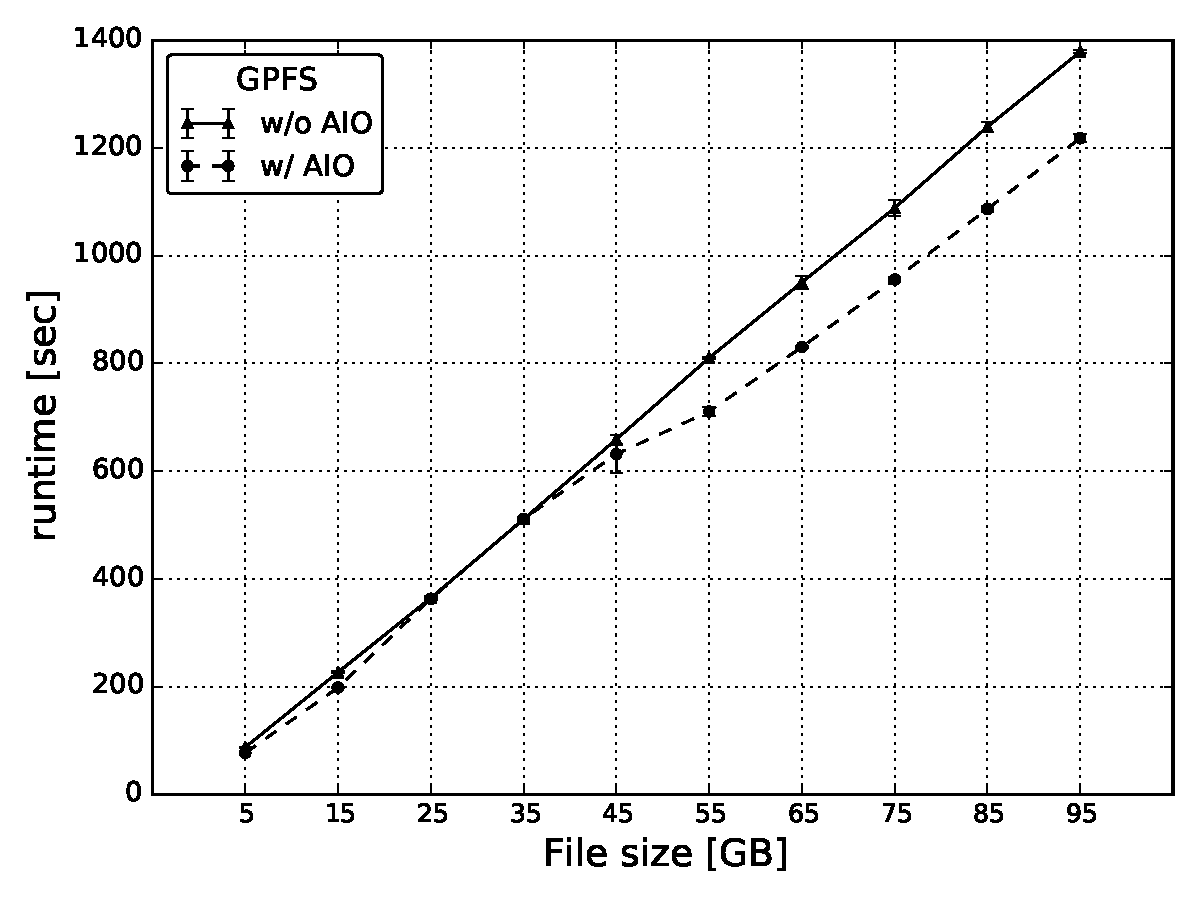
\includegraphics[width=\textwidth]{figures/gpfs/runtime}
%    \caption{\textit{}}
%    \label{figure: gpfs_1}
%  \end{subfigure}
%  \begin{subfigure}[t]{0.48\textwidth}
%    \centering
%    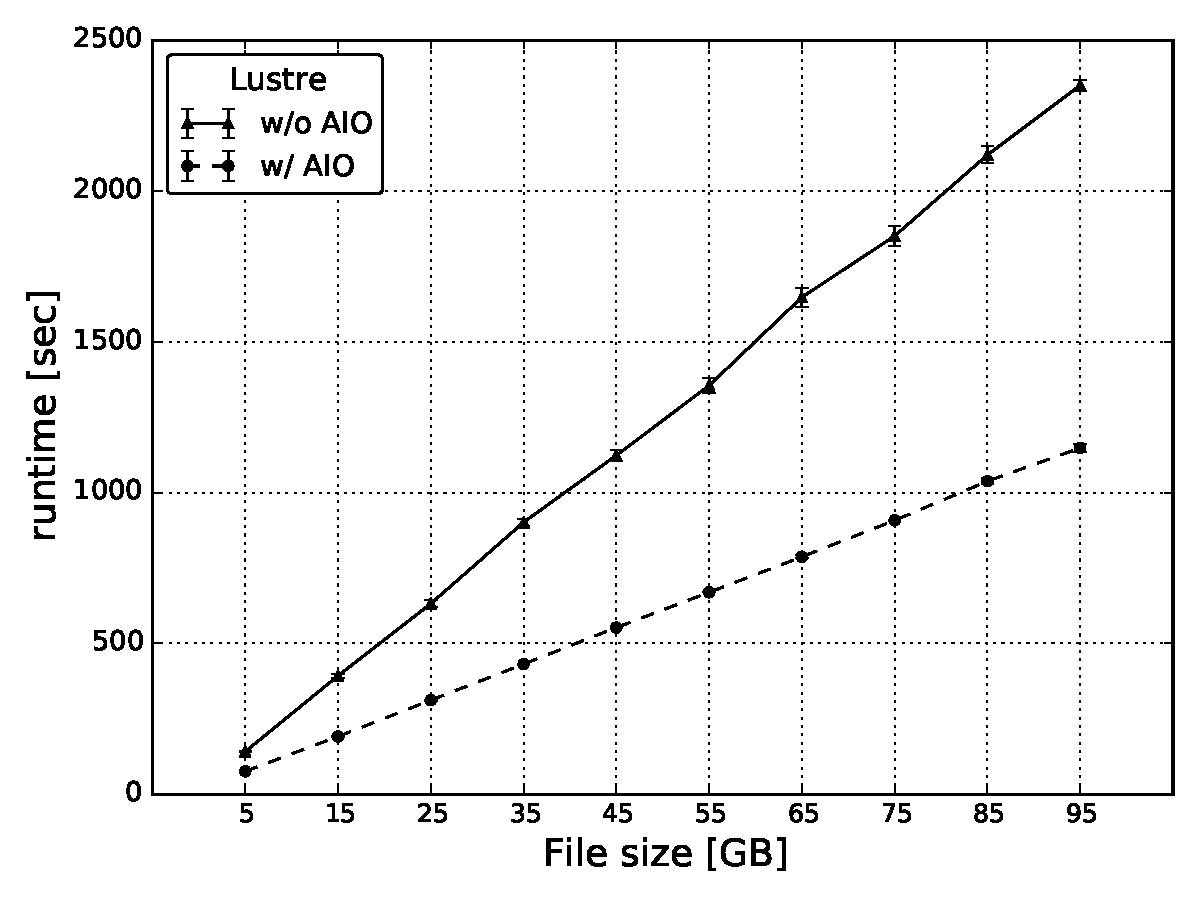
\includegraphics[width=\textwidth]{figures/Lustre/runtime}
%    \caption{\textit{}}
%    \label{figure: lustre_1}
%  \end{subfigure}
%  \caption{Running time of the ROOT application for the three file systems under study using different input file sized (\ref{figure: ext4_1},~\ref{figure: gpfs_1} and~\ref{figure: lustre_1}).}
%  \label{figure: run-time_1}
%\end{figure}
%
%\begin{figure}[!htb]
%  \centering
%  \begin{subfigure}[b]{0.48\textwidth}
%    \centering
%    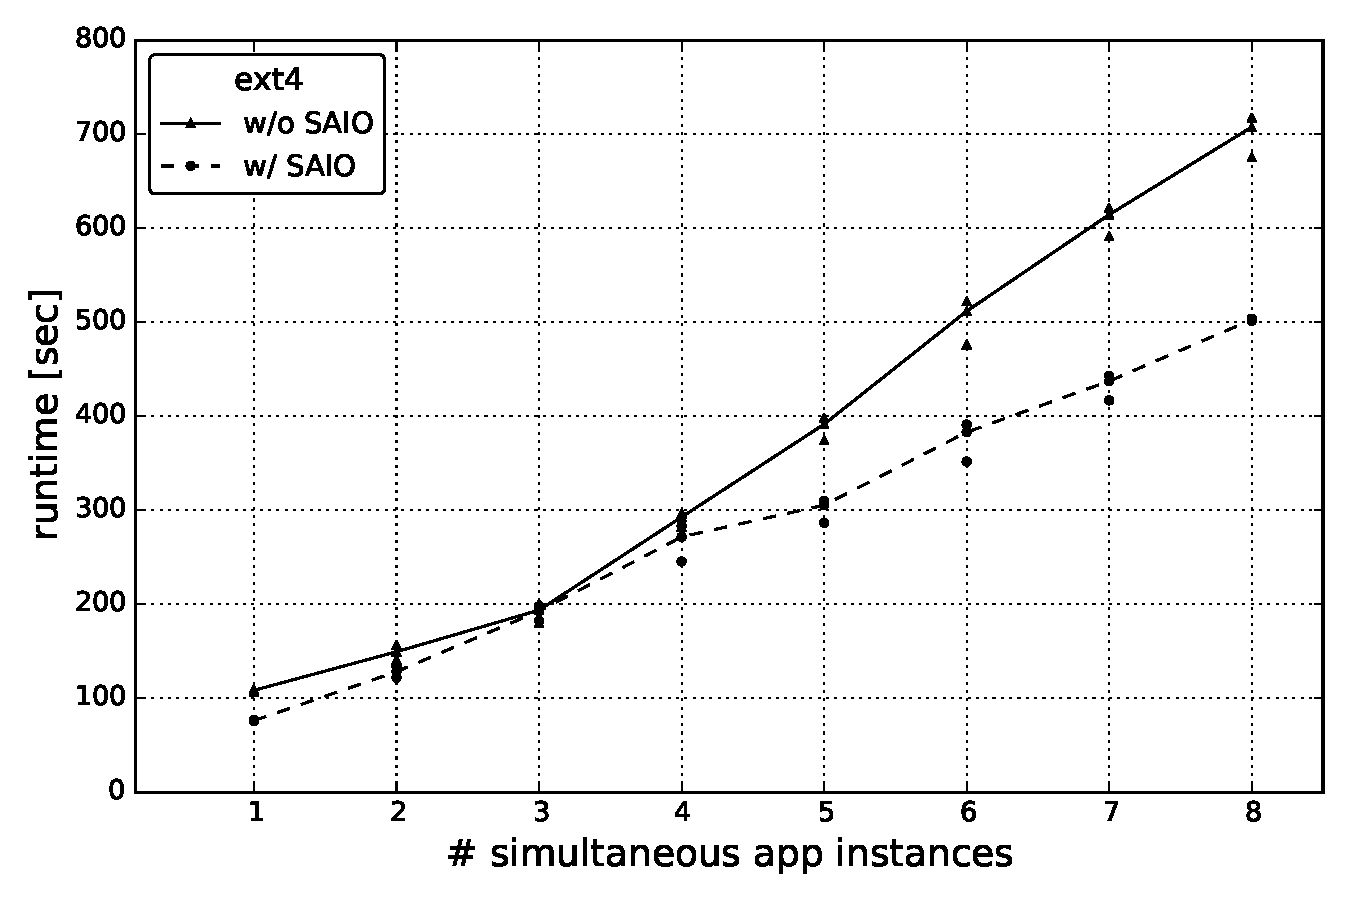
\includegraphics[width=\textwidth]{figures/simult_instance_ext4_test_cluster}
%    \caption{\textit{}}
%    \label{figure: ext4_2}
%  \end{subfigure}
%  \begin{subfigure}[b]{0.48\textwidth}
%    \centering
%    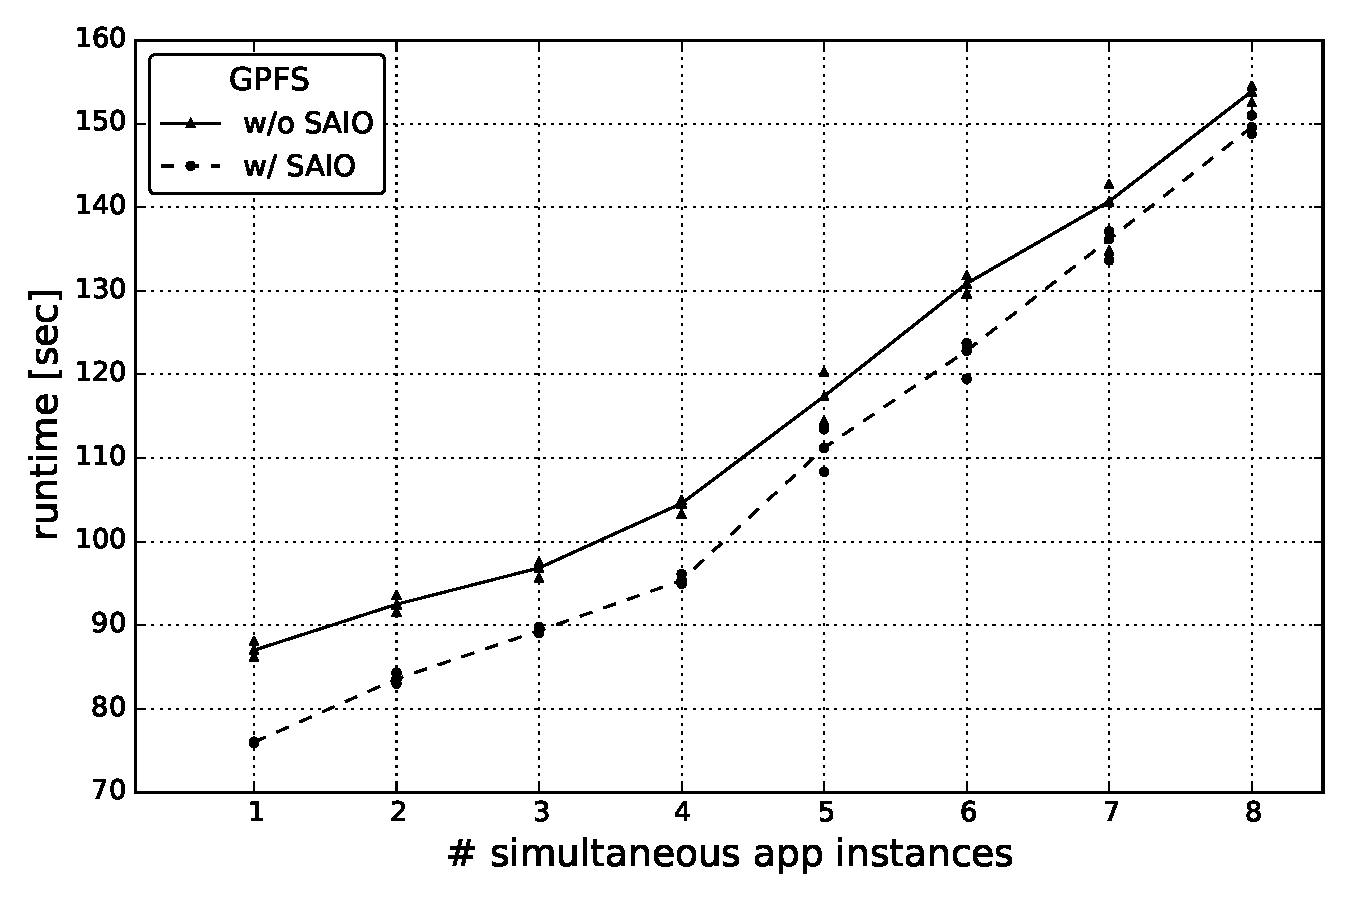
\includegraphics[width=\textwidth]{figures/simult_instance_gpfs_test_cluster}
%    \caption{\textit{}}
%    \label{figure: gpfs_2}
%  \end{subfigure}
%  \begin{subfigure}[b]{0.48\textwidth}
%    \centering
%    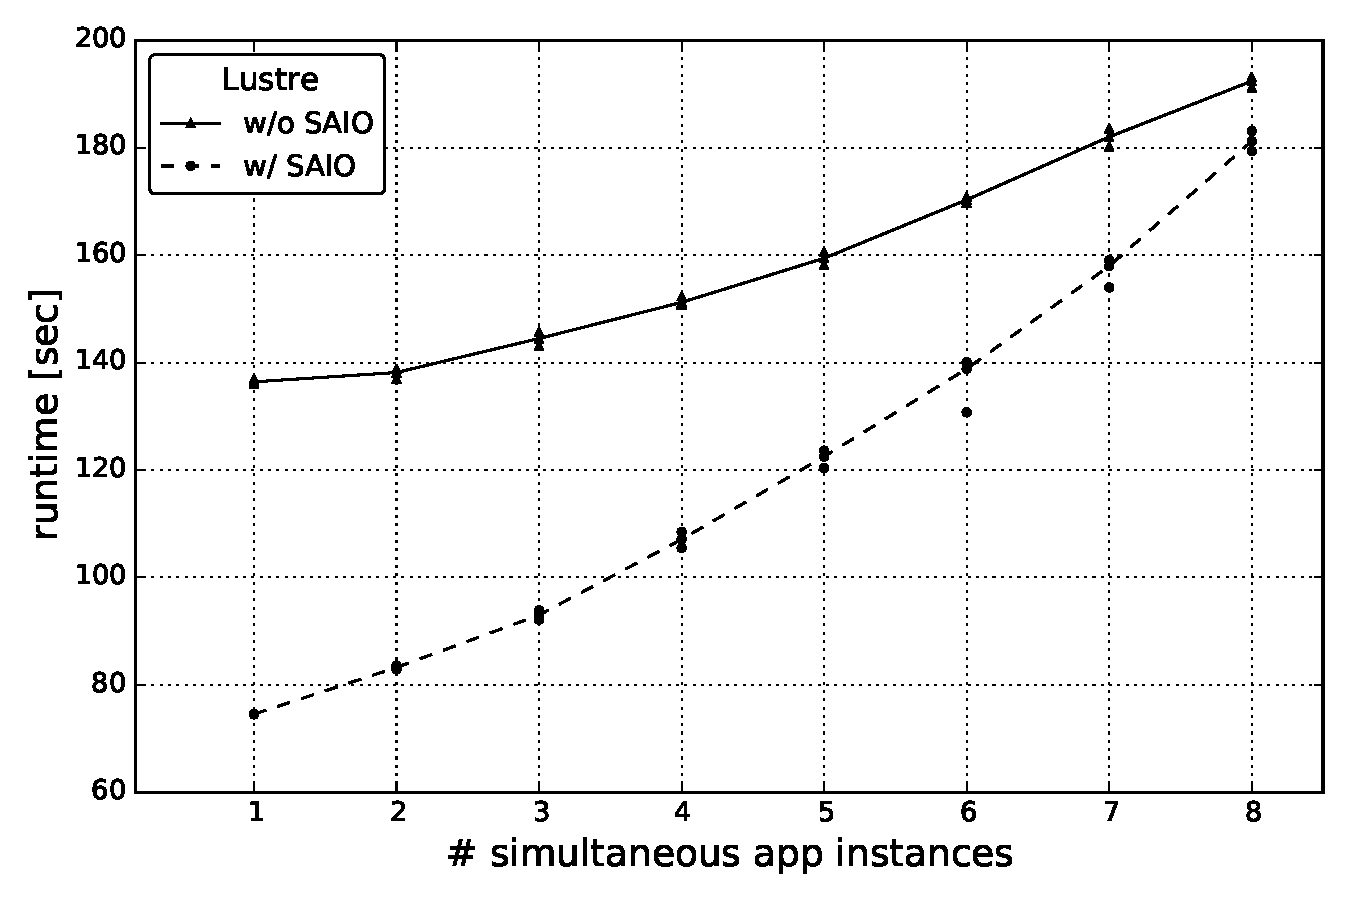
\includegraphics[width=\textwidth]{figures/multiple_simult_procs_Lustre_testcluster}
%    \caption{\textit{}}
%    \label{figure: lustre_2}
%  \end{subfigure}
%  \caption{Running time of the ROOT application for the three file system under study using different of application instances accessing a file of 5 GB (\ref{figure: ext4_2},~\ref{figure: gpfs_2} and~\ref{figure: lustre_2}).}
%  \label{figure: run-time_2}
%\end{figure}
%
%\begin{figure}[!htb]
%  \centering
%  \begin{subfigure}[t]{0.48\textwidth}
%    \centering
%    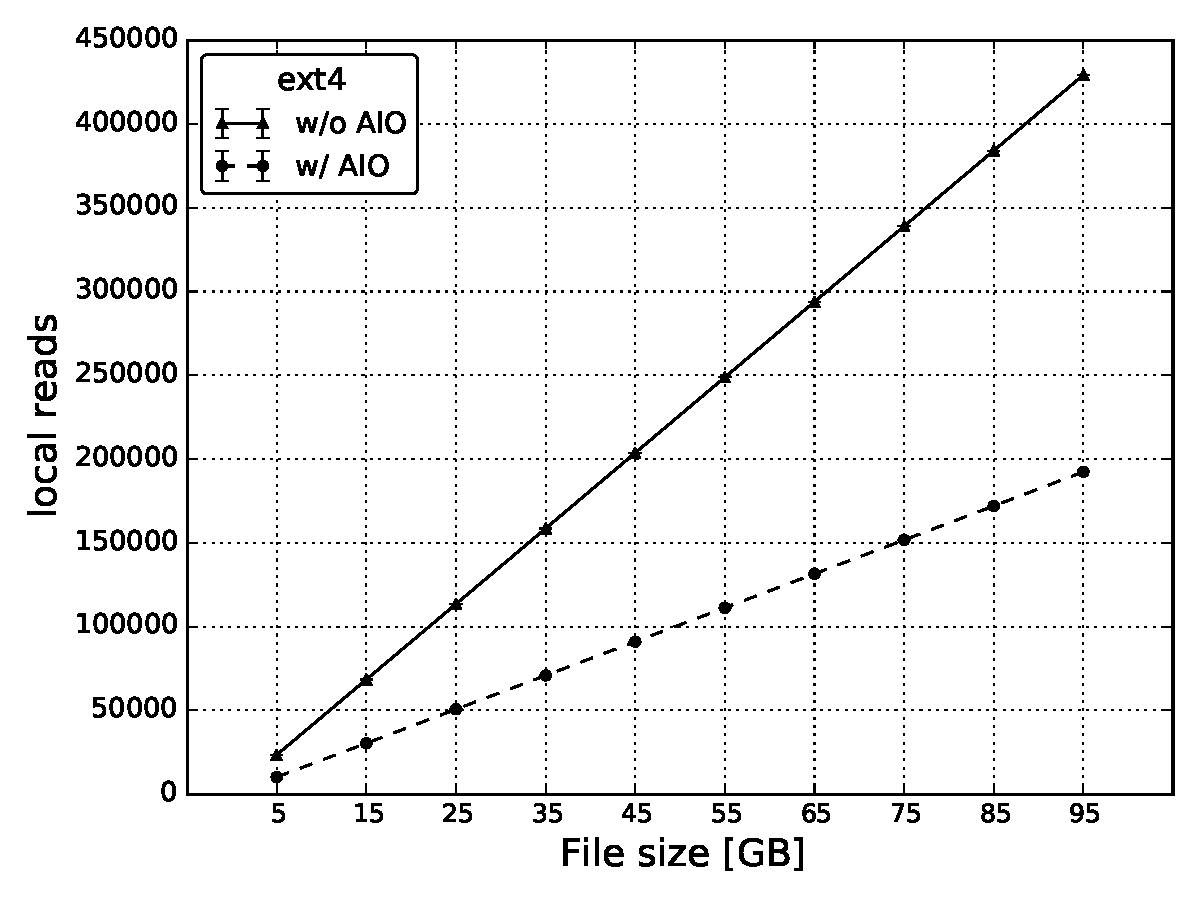
\includegraphics[width=\textwidth]{figures/ext4/reads}
%    \caption{\textit{}}
%    \label{figure: ext4_3}
%  \end{subfigure}
%  \begin{subfigure}[t]{0.48\textwidth}
%    \centering
%    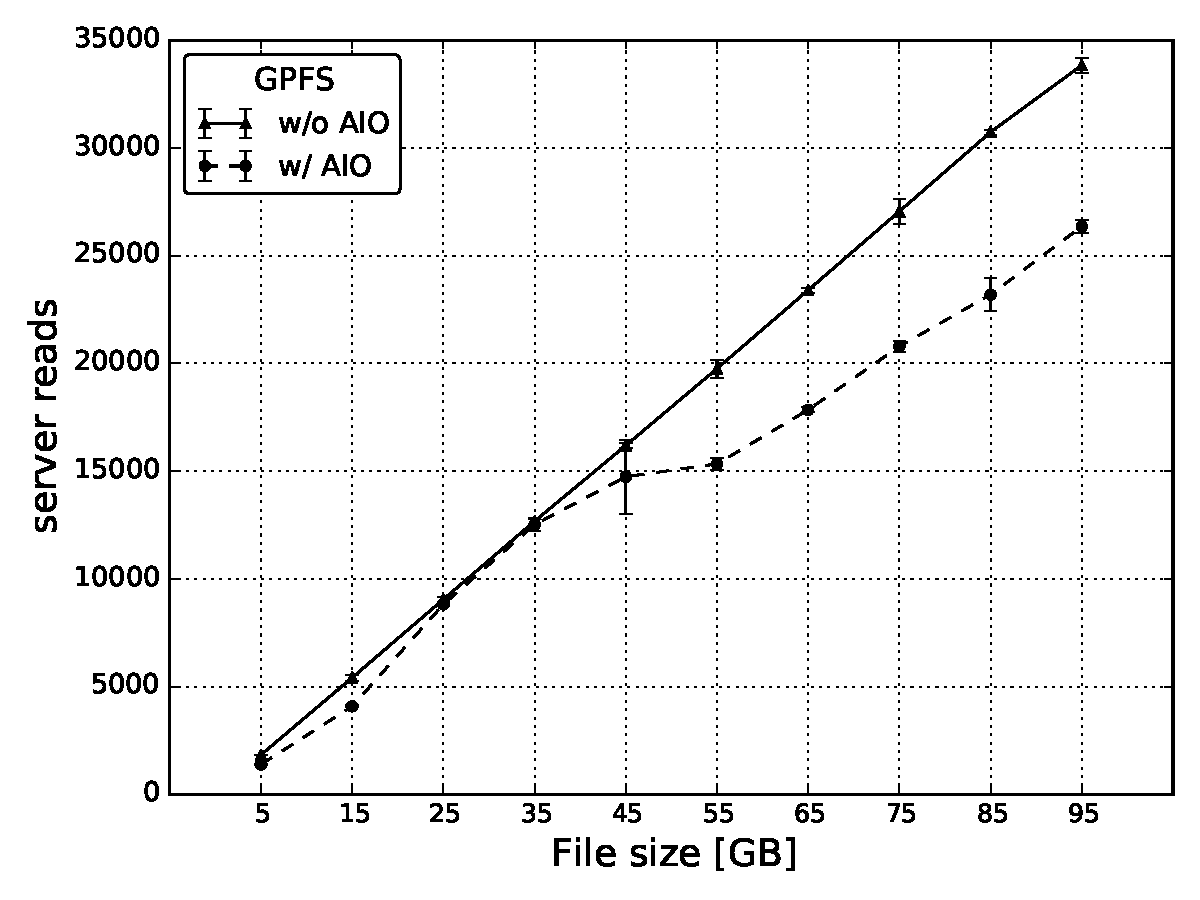
\includegraphics[width=\textwidth]{figures/gpfs/server_reads}
%    \caption{\textit{}}
%    \label{figure: gpfs_3}
%  \end{subfigure}
%  \begin{subfigure}[t]{0.48\textwidth}
%    \centering
%    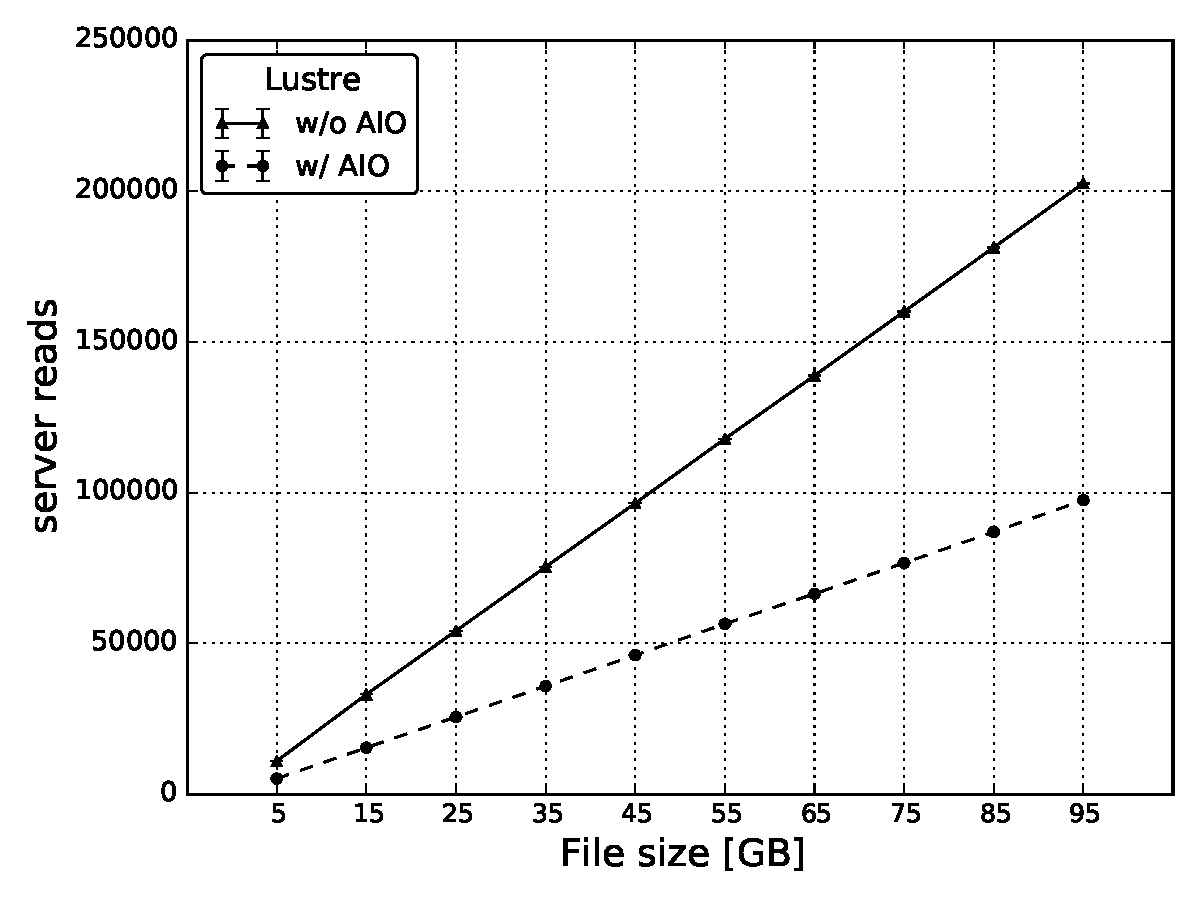
\includegraphics[width=\textwidth]{figures/Lustre/server_reads}
%    \caption{\textit{}}
%    \label{figure: lustre_3}
%  \end{subfigure}
%  \caption{Reads processed by local ext4, GPFS and Lustre I/O servers for various input file sizes (\ref{figure: ext4_3},~\ref{figure: gpfs_3} and~\ref{figure: lustre_3}).}
%  \label{figure: read_1}
%\end{figure}
%
%\begin{figure}[!htb]
%  \centering
%  \begin{subfigure}[b]{0.48\textwidth}
%    \centering
%    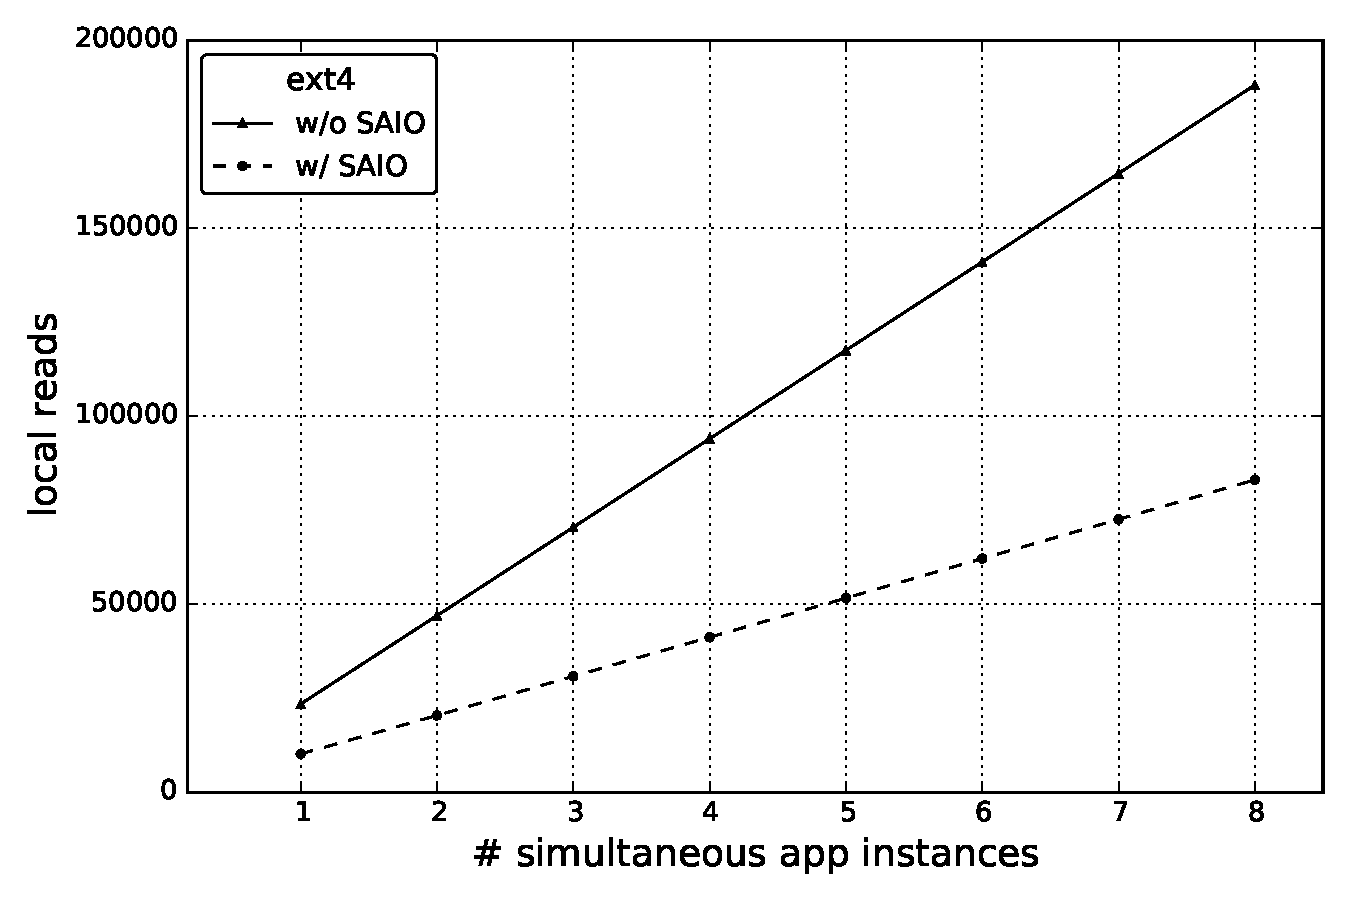
\includegraphics[width=\textwidth]{figures/reads_simult_instance_ext4_test_cluster}
%    \caption{\textit{}}
%    \label{figure: ext4_4}
%  \end{subfigure}
%  \begin{subfigure}[b]{0.48\textwidth}
%    \centering
%    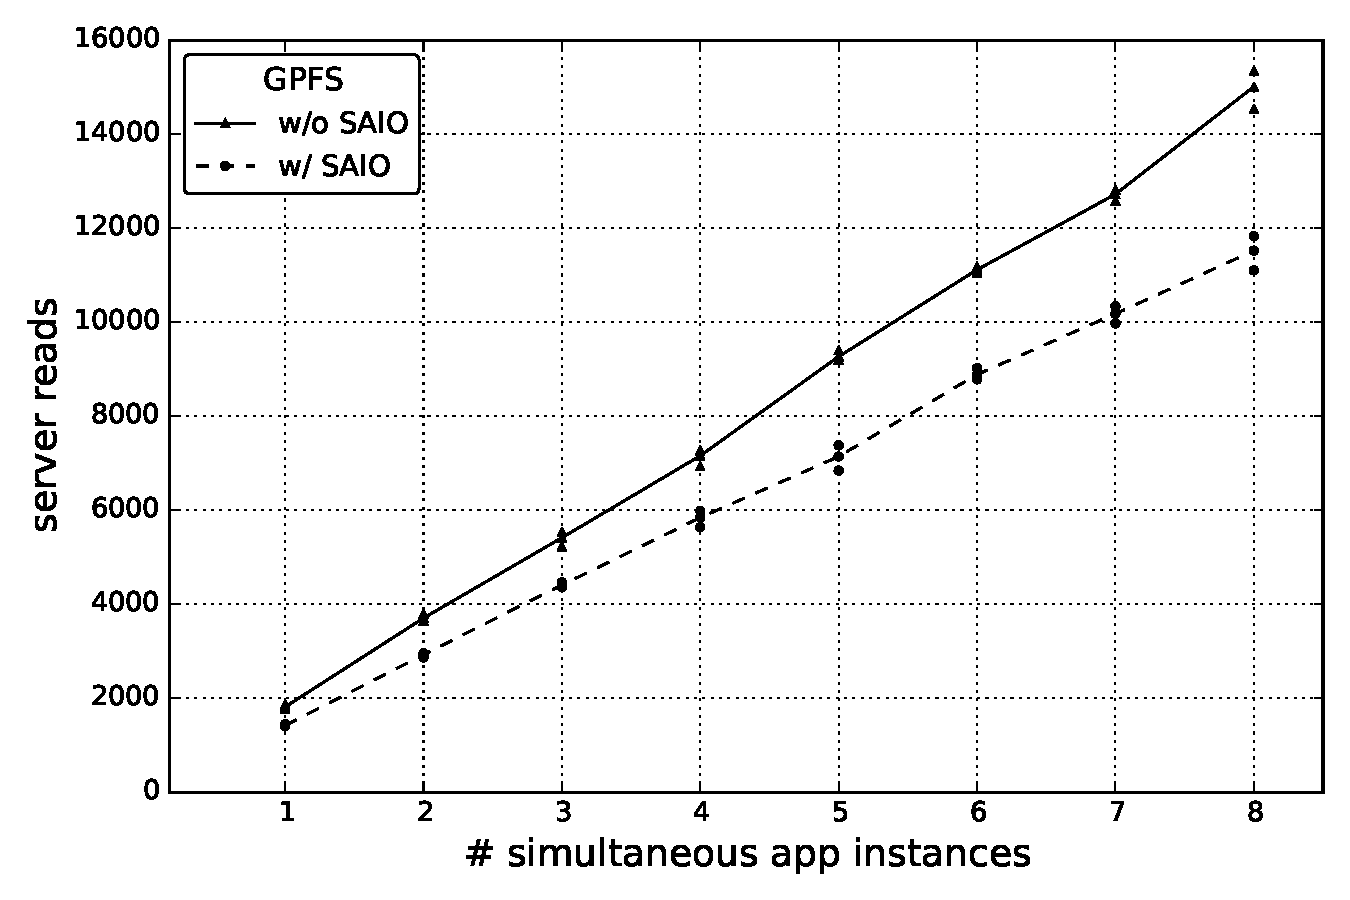
\includegraphics[width=\textwidth]{figures/reads_simult_instance_gpfs_test_cluster}
%    \caption{\textit{}}
%    \label{figure: gpfs_4}
%  \end{subfigure}
%  \begin{subfigure}[b]{0.48\textwidth}
%    \centering
%    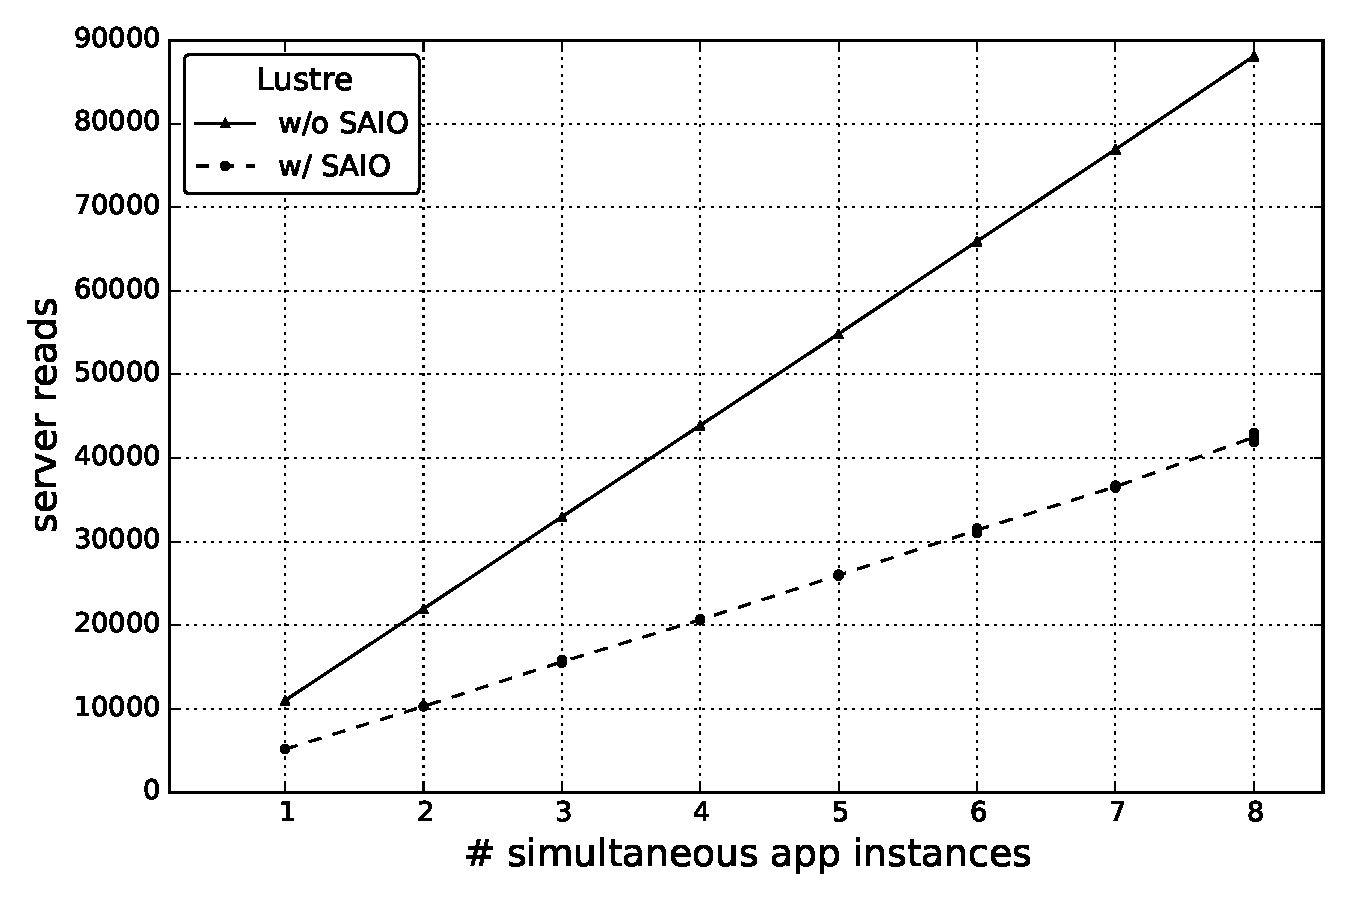
\includegraphics[width=\textwidth]{figures/reads_multiple_simult_procs_Lustre_testcluster}
%    \caption{\textit{}}
%    \label{figure: lustre_4}
%  \end{subfigure}
%  \caption{Reads processed by local ext4, GPFS and Lustre I/O servers for multiple instances of ROOT accessing a file of 5 GB (\ref{figure: ext4_4},~\ref{figure: gpfs_4} and~\ref{figure: lustre_4}).}
%  \label{figure: read_2}
%\end{figure}

\begin{figure*}[]
  \centering
  \begin{subfigure}[]{0.70\textwidth}
    \centering
    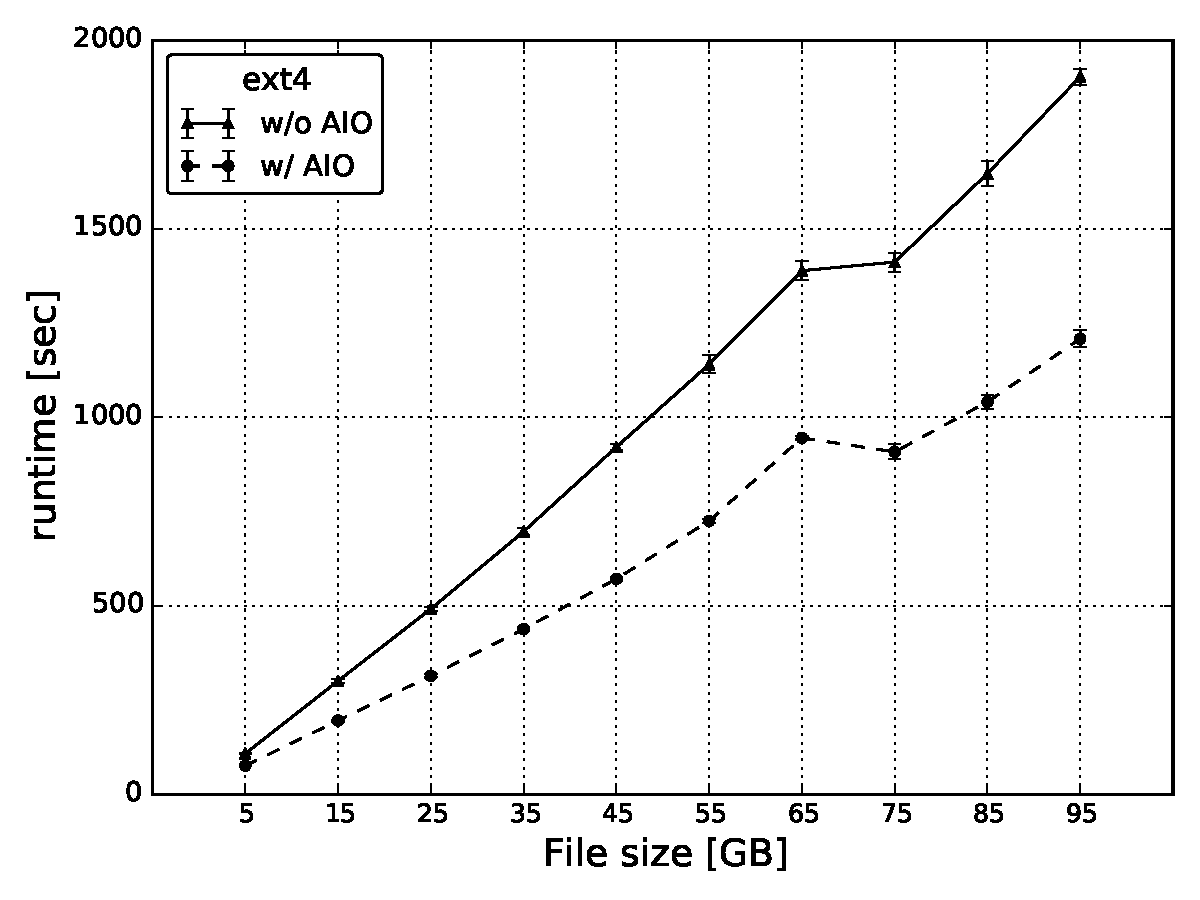
\includegraphics[width=\textwidth]{figures/ext4/runtime}
    \caption{\textit{}}
    \label{figure: ext4_1}
  \end{subfigure}
  \begin{subfigure}[]{0.70\textwidth}
    \centering
    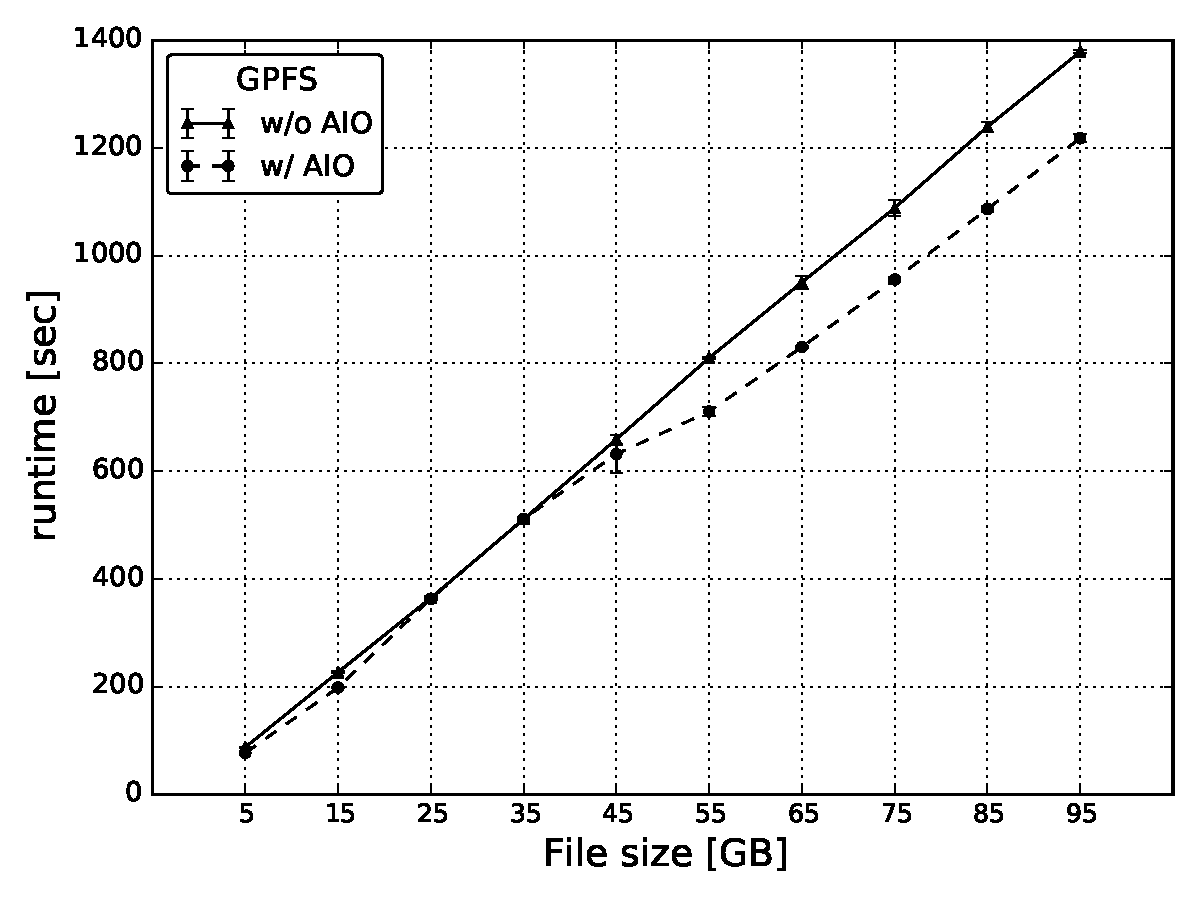
\includegraphics[width=\textwidth]{figures/gpfs/runtime}
    \caption{\textit{}}
    \label{figure: gpfs_1}
  \end{subfigure}
  \begin{subfigure}[]{0.70\textwidth}
    \centering
    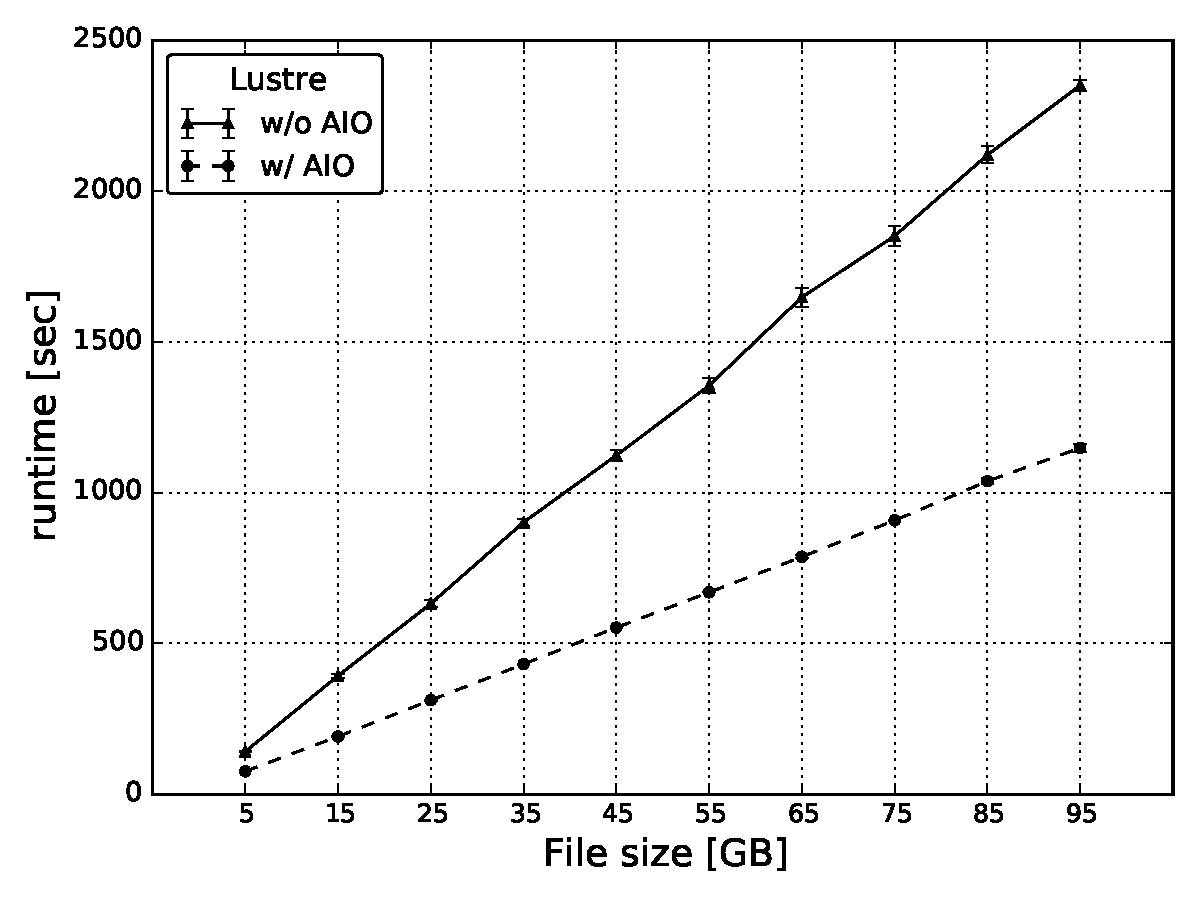
\includegraphics[width=\textwidth]{figures/Lustre/runtime}
    \caption{\textit{}}
    \label{figure: lustre_1}
  \end{subfigure}
  \caption{Running time of the ROOT application for the three file systems under study using different input file sized (\ref{figure: ext4_1},~\ref{figure: gpfs_1} and~\ref{figure: lustre_1}).}
  \label{figure: run-time_1}
\end{figure*}

\begin{figure*}[]
  \centering
  \begin{subfigure}[]{0.70\textwidth}
    \centering
    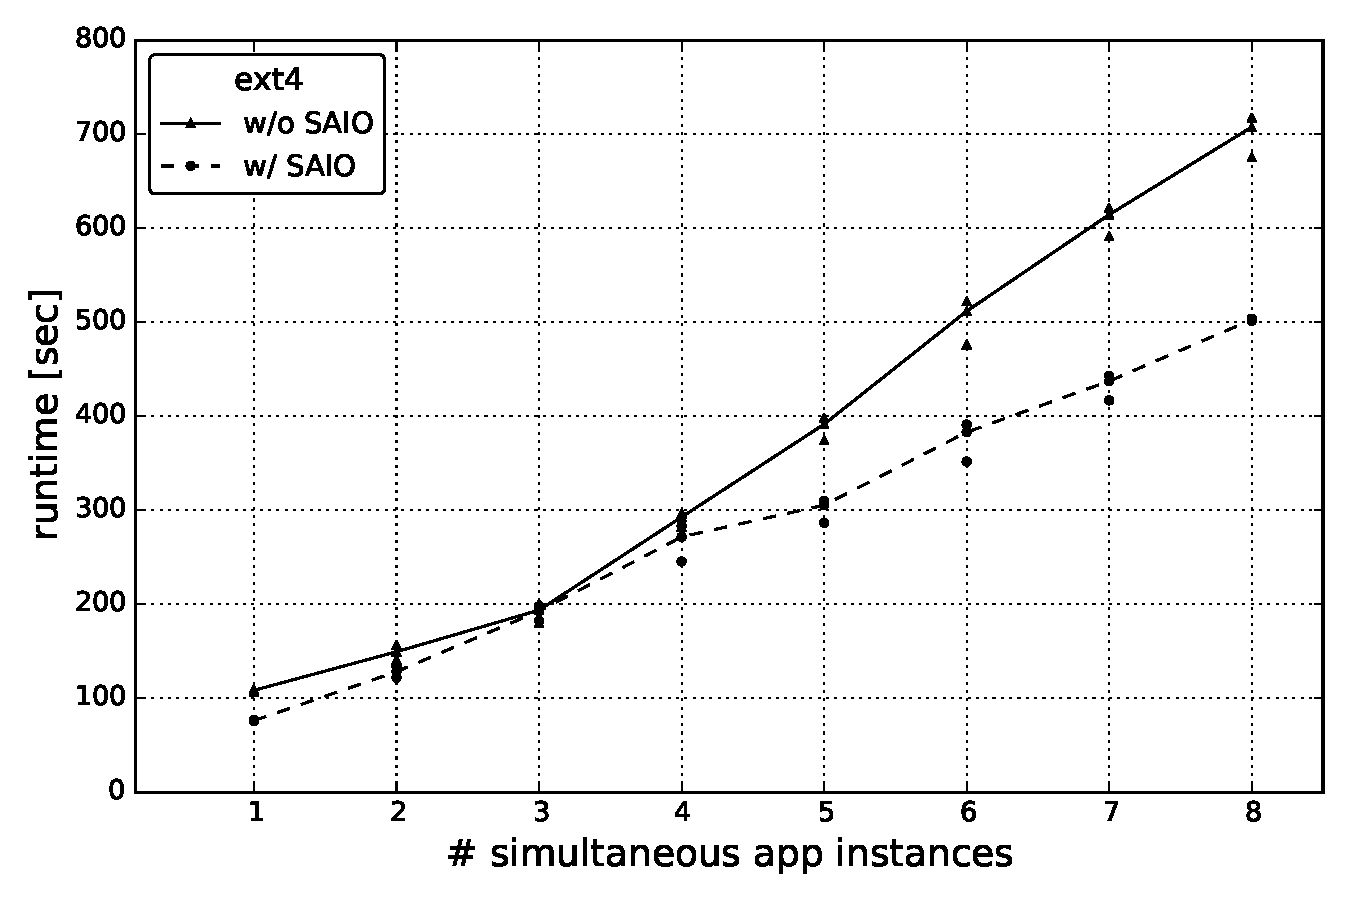
\includegraphics[width=\textwidth]{figures/simult_instance_ext4_test_cluster}
    \caption{\textit{}}
    \label{figure: ext4_2}
  \end{subfigure}
  \begin{subfigure}[]{0.70\textwidth}
    \centering
    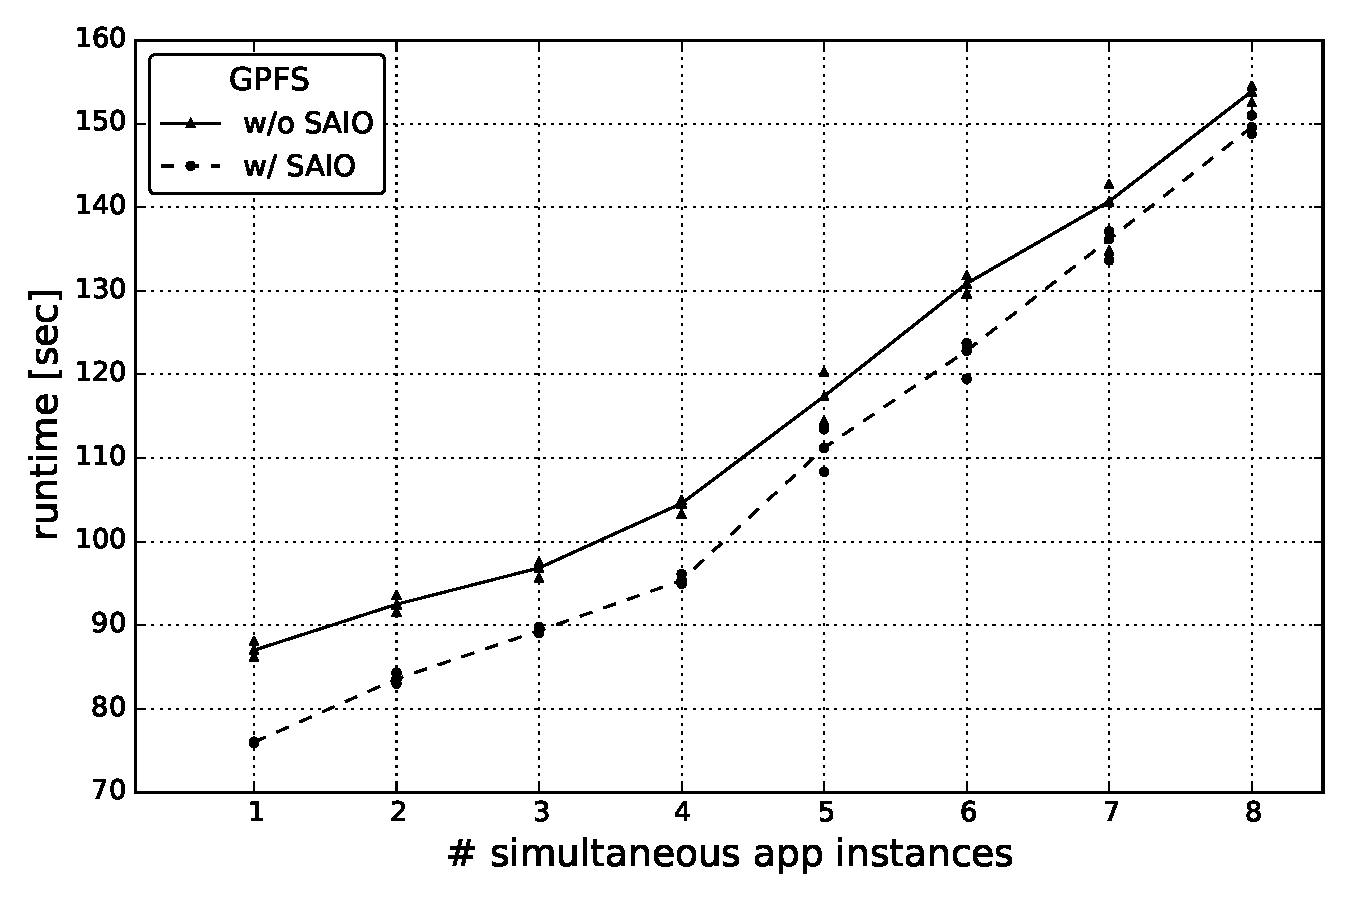
\includegraphics[width=\textwidth]{figures/simult_instance_gpfs_test_cluster}
    \caption{\textit{}}
    \label{figure: gpfs_2}
  \end{subfigure}
  \begin{subfigure}[]{0.70\textwidth}
    \centering
    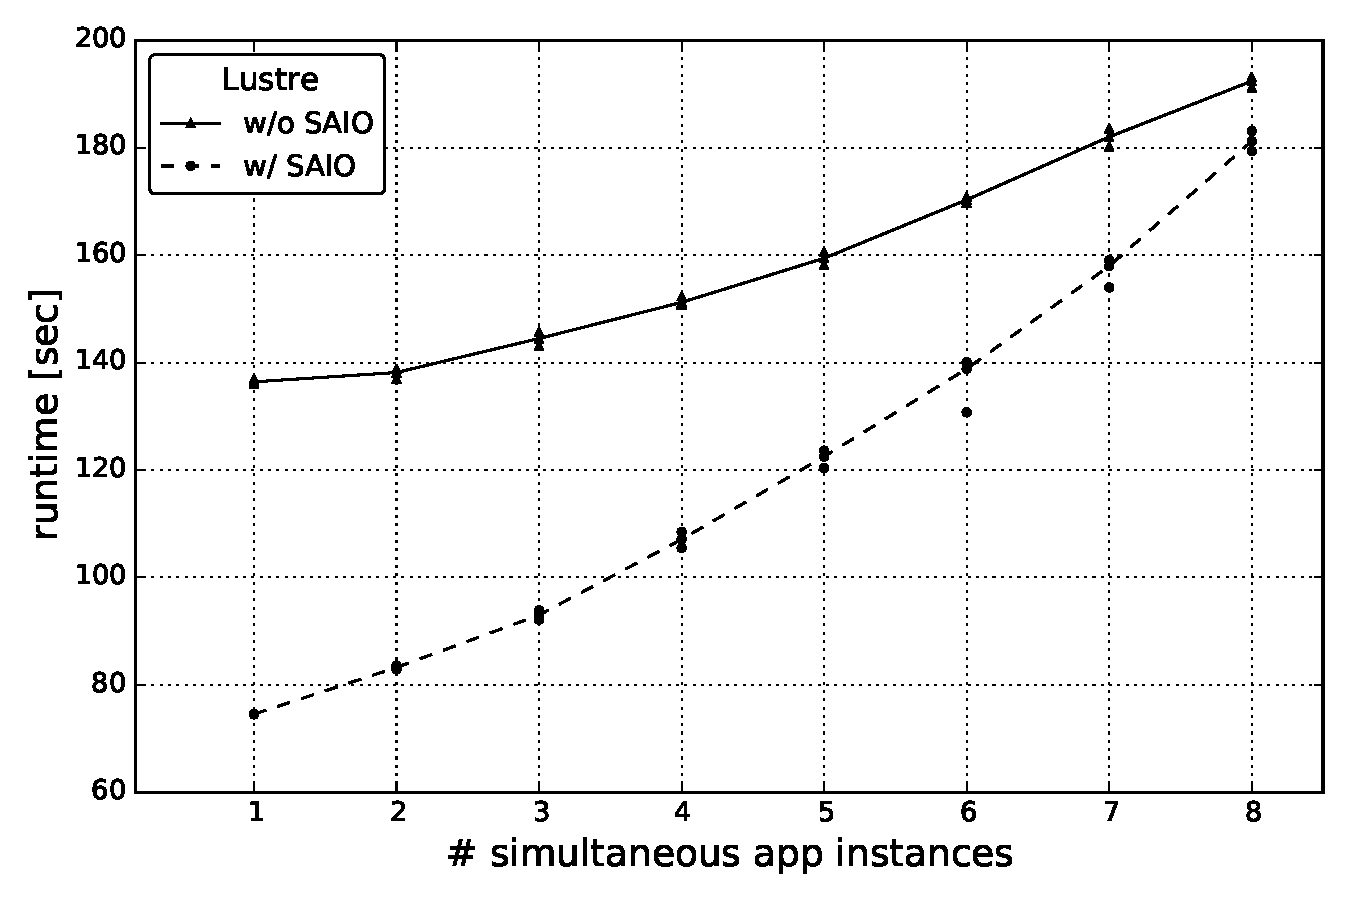
\includegraphics[width=\textwidth]{figures/multiple_simult_procs_Lustre_testcluster}
    \caption{\textit{}}
    \label{figure: lustre_2}
  \end{subfigure}
  \caption{Running time of the ROOT application for the three file system under study using different of application instances accessing a file of 5 GB (\ref{figure: ext4_2},~\ref{figure: gpfs_2} and~\ref{figure: lustre_2}).}
  \label{figure: run-time_2}
\end{figure*}

\begin{figure*}[]
  \centering
  \begin{subfigure}[]{0.70\textwidth}
    \centering
    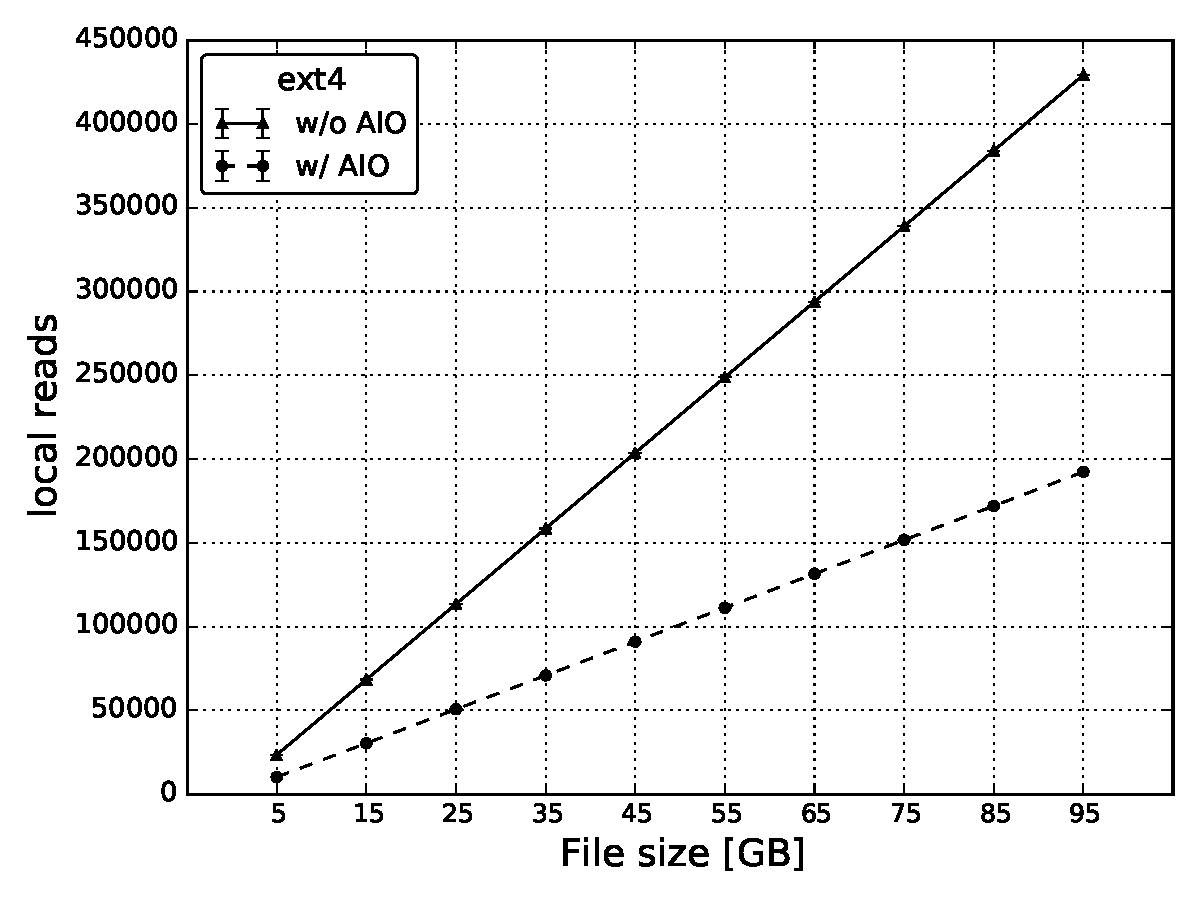
\includegraphics[width=\textwidth]{figures/ext4/reads}
    \caption{\textit{}}
    \label{figure: ext4_3}
  \end{subfigure}
  \begin{subfigure}[]{0.70\textwidth}
    \centering
    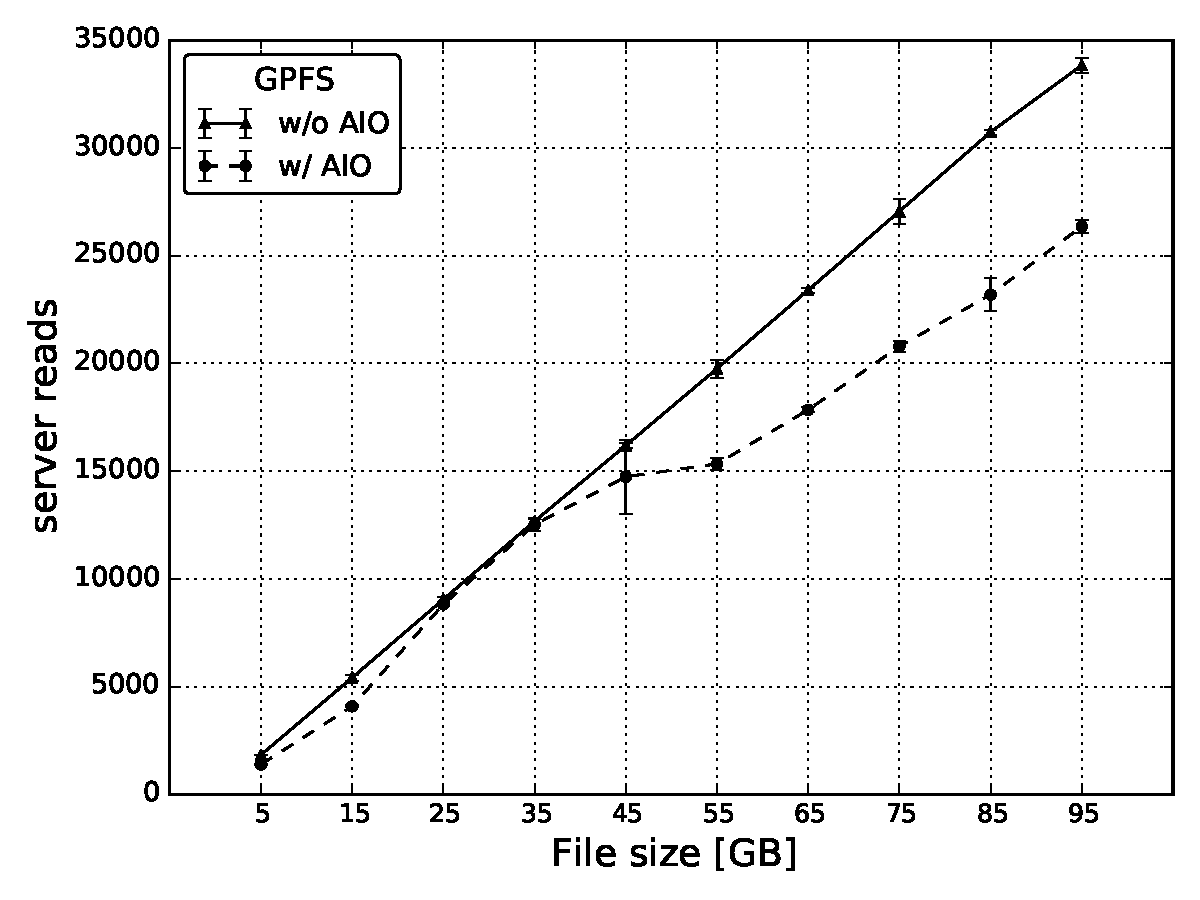
\includegraphics[width=\textwidth]{figures/gpfs/server_reads}
    \caption{\textit{}}
    \label{figure: gpfs_3}
  \end{subfigure}
  \begin{subfigure}[]{0.70\textwidth}
    \centering
    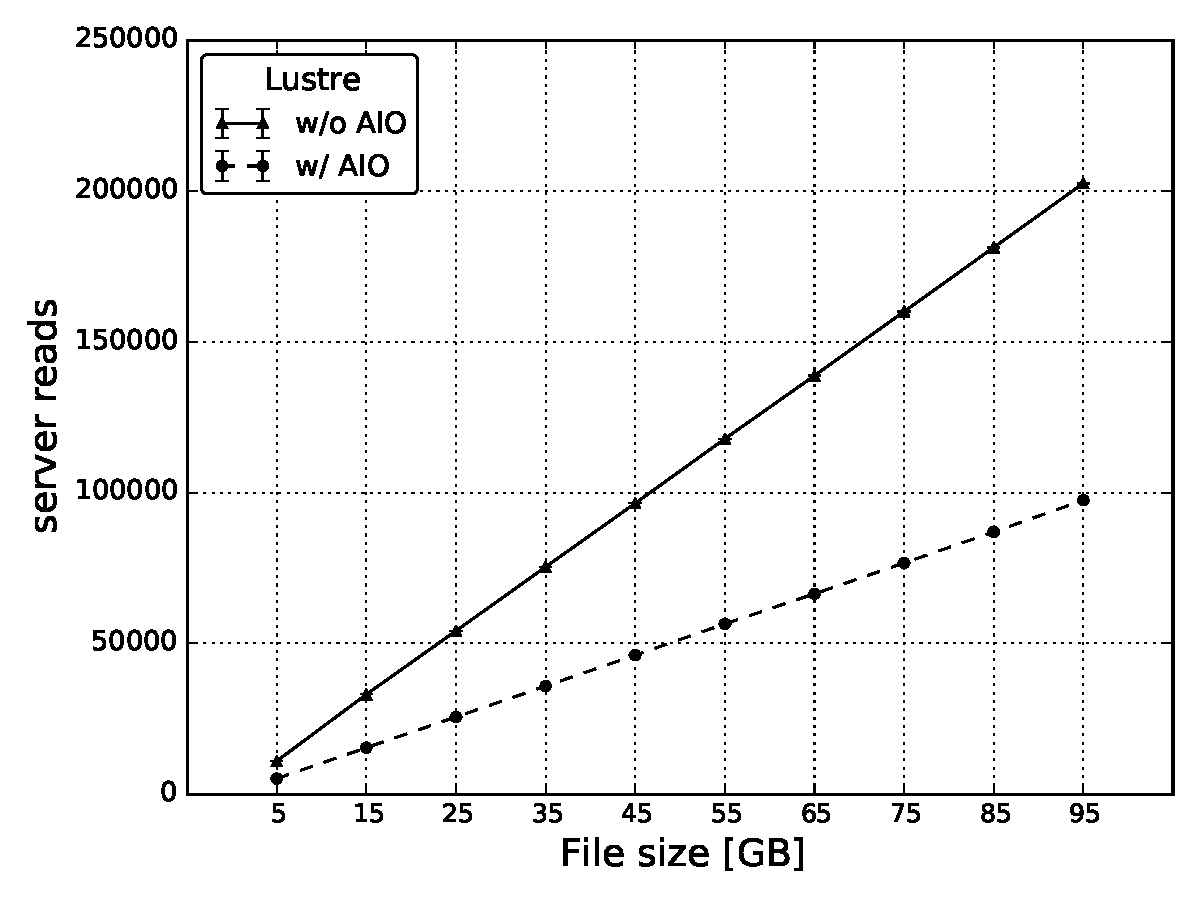
\includegraphics[width=\textwidth]{figures/Lustre/server_reads}
    \caption{\textit{}}
    \label{figure: lustre_3}
  \end{subfigure}
  \caption{Reads processed by local ext4, GPFS and Lustre I/O servers for various input file sizes (\ref{figure: ext4_3},~\ref{figure: gpfs_3} and~\ref{figure: lustre_3}).}
  \label{figure: read_1}
\end{figure*}

\begin{figure*}[]
  \centering
  \begin{subfigure}[]{0.70\textwidth}
    \centering
    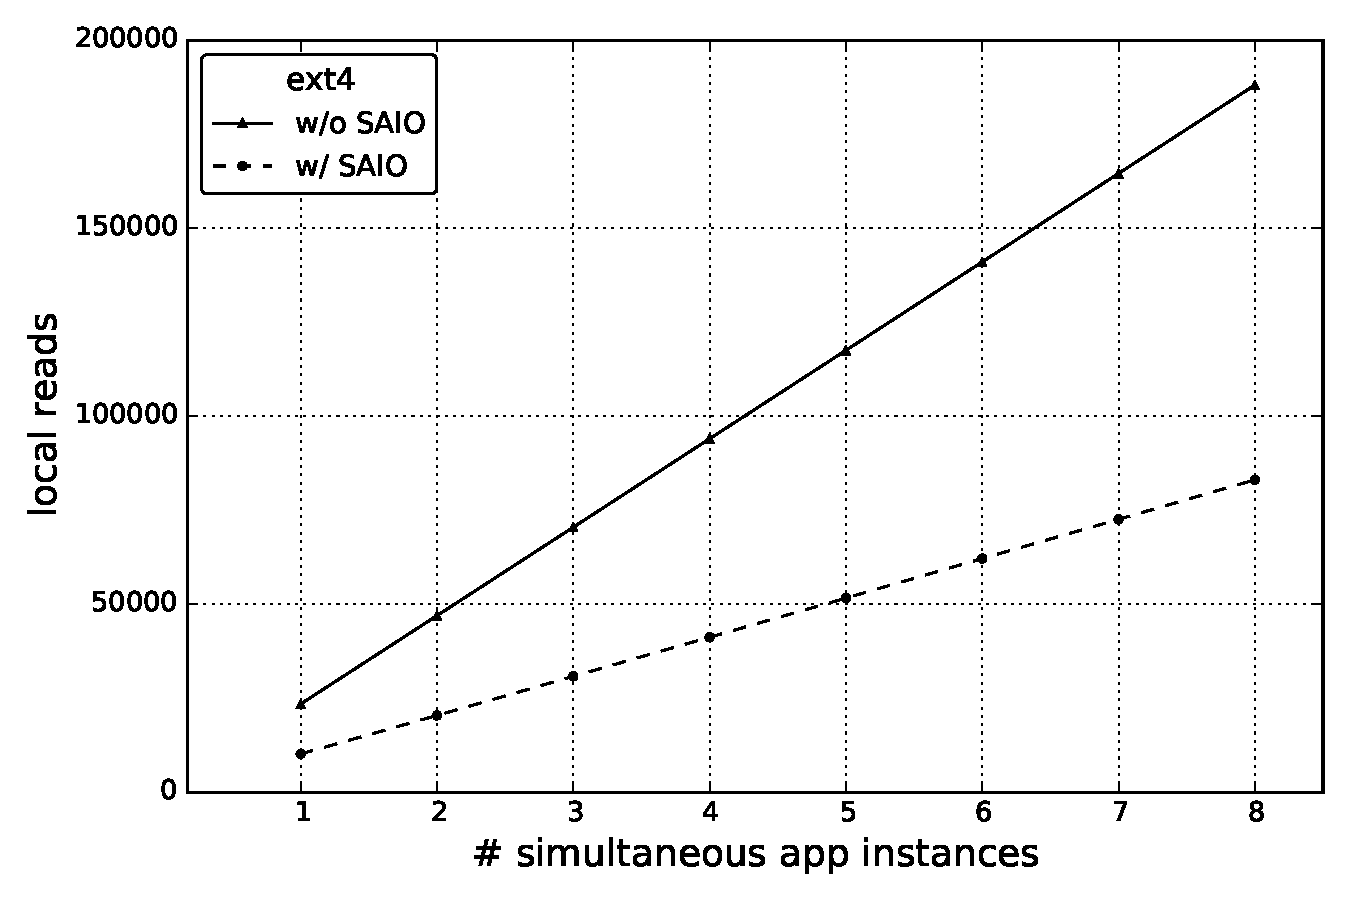
\includegraphics[width=\textwidth]{figures/reads_simult_instance_ext4_test_cluster}
    \caption{\textit{}}
    \label{figure: ext4_4}
  \end{subfigure}
  \begin{subfigure}[]{0.70\textwidth}
    \centering
    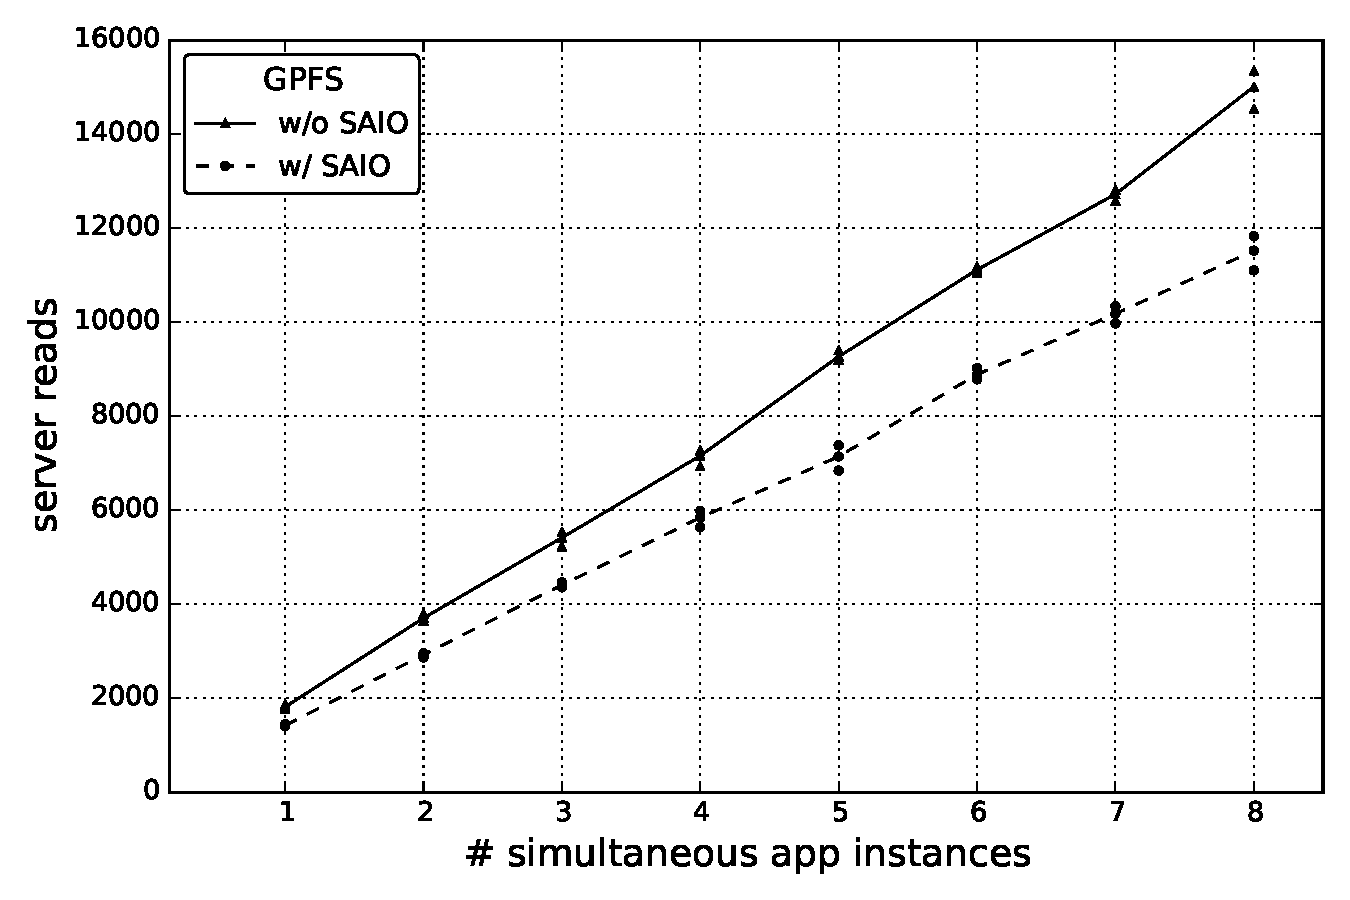
\includegraphics[width=\textwidth]{figures/reads_simult_instance_gpfs_test_cluster}
    \caption{\textit{}}
    \label{figure: gpfs_4}
  \end{subfigure}
  \begin{subfigure}[]{0.70\textwidth}
    \centering
    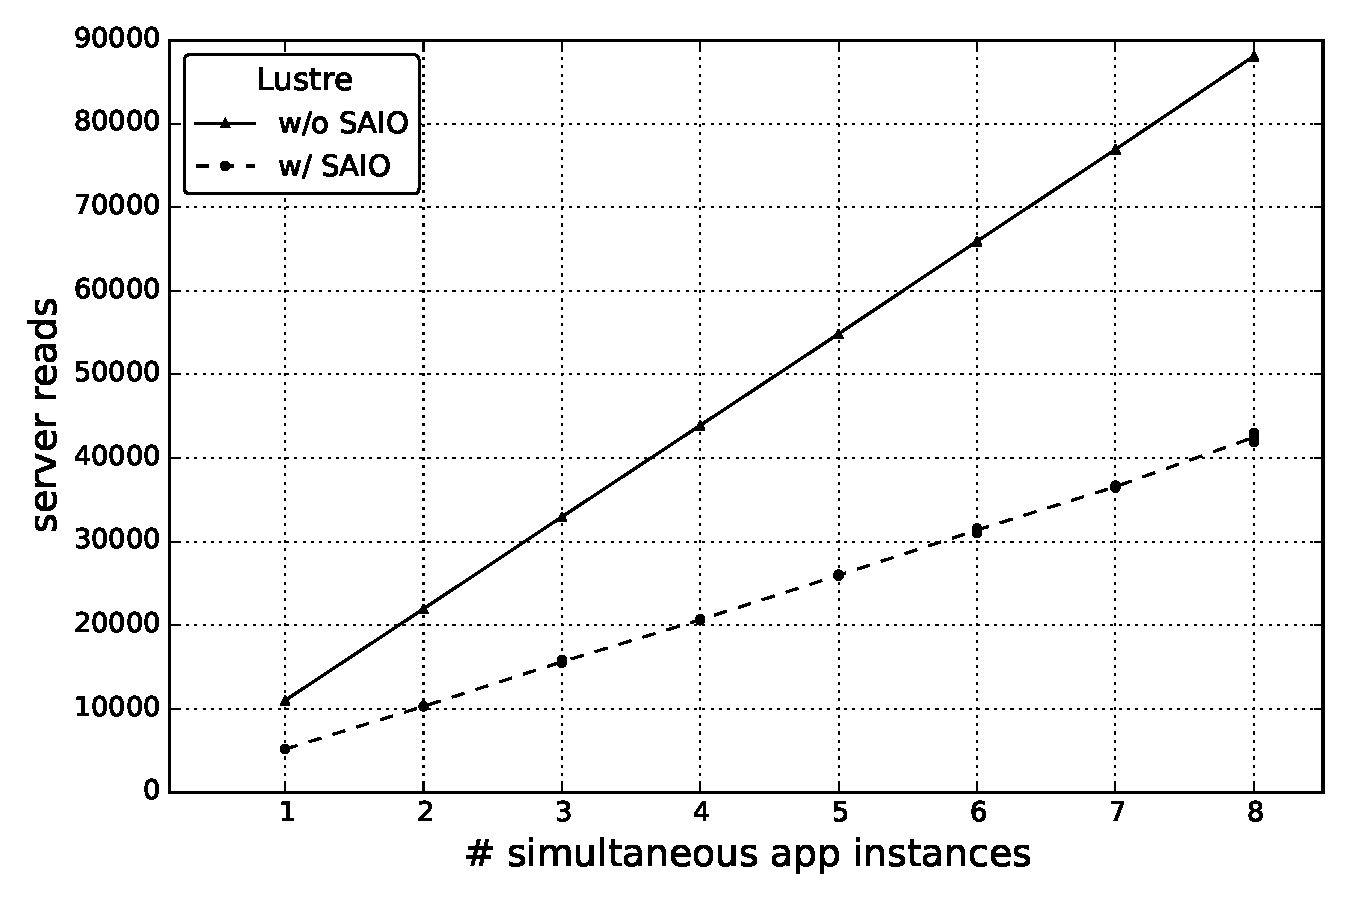
\includegraphics[width=\textwidth]{figures/reads_multiple_simult_procs_Lustre_testcluster}
    \caption{\textit{}}
    \label{figure: lustre_4}
  \end{subfigure}
  \caption{Reads processed by local ext4, GPFS and Lustre I/O servers for multiple instances of ROOT accessing a file of 5 GB (\ref{figure: ext4_4},~\ref{figure: gpfs_4} and~\ref{figure: lustre_4}).}
  \label{figure: read_2}
\end{figure*}

As far as Figures~\ref{figure: ext4_2},~\ref{figure: gpfs_2} and~\ref{figure: lustre_2} are concerned, these account for the effect of processes' concurrency on the file system. 
Before continuing with the discussion we have to make a note here. In our architecture, only one process per file system's client issues (through multiple \textit{Advisor Thread}s) 
hints on behalf of running applications. This introduces some overhead, since we have to pass the access information from the \textit{Assisted I/O library} to the \textit{Advice Manager}, 
but has the advantage of better coordinating accesses to the same file from multiple processes. Nevertheless, we found that in the case of GPFS, despite the fact of having multiple 
\textit{Advisor Thread}s, only one process among the many was receiving a benefit from the prefetching hints; the reason is that GPFS seems to have the restriction of hinting only one 
file per process. For this reason, we developed another variant of Mercury in which the AIO library, now renamed \textit{Self Assisted I/O library} (SAIO), internally provides the 
creation and the handling of multiple \textit{Advisor Thread}s. 

Looking at the figures generated with the new SAIO library we can assess the effectiveness of the prefetching hints for 
the three file systems considered. In particular, Lustre provides the best run-time improvements compared to the case in which no hints were used. GPFS shows a more contained improvement 
since the I/O time is already small compared to Lustre and ext4. Finally, ext4 can really benefit from prefetching hints especially for high process counts. Overall, excluding ext4, when 
we increase the number of processes the run-time improvements shrink. Because ext4 transfers data directly from the local SATA HDD, in which I/O time is dominated by disk latency, we can 
still improve performance as the number of application instances increases by making efficient use of the cache to hide such latency. GPFS and Lustre servers, on the other hand, have much 
higher transfer performance compared to single disk ext4 and both use a network link to move data across the network; GPFS uses the NSD protocol while Lustre uses the LNET protocol. For GPFS
and Lustre network bandwidth becomes critical and, in fact, as the number of instances increases the run-time decreases because of the saturation of the network link in the node.

Figure~\ref{figure: ext4_3},~\ref{figure: gpfs_3} and~\ref{figure: lustre_3} report the number of read requests accounted for by the different file systems under study. More specifically, 
the figures show how the number of reads at the I/O server side for both GPFS and Lustre can be substantially reduced with our approach. This has a significant impact in HPC cluster in 
which the file system may be accessed by many thousand of processes at the same time. Reducing the number of requests for an application can increase the number of IOPS available for others. 
This result is also confirmed for multiple instances of the `ROOT' application running concurrently (Figure~\ref{figure: ext4_4},~\ref{figure: gpfs_4} and~\ref{figure: lustre_4}).

\subsection{Conclusions}
Our experiments have focused on prefetching performance in a real scenario setup. In particular we have considered the cache utilization by a single application's instance as well as the
combined cache utilization by multiple application's instances. We have shown how in both cases we can reduce the application runtime by aggressively prefetching data into main memory using
our transparent approach. However, since our strategy is bandwidth bound we have seen that in the case of multiple application's instances such approach leads to the saturation of the
network link in the case of networked file systems and ultimately to the shrinking of the performance gain.

%One important aspect to consider in HPC is that although nodes typically run only a single application at a time, there might
%be still multiple instances of it operating on different parts of the input dataset (SPMD model). As we have mentioned in Chapter~\ref{chapt: introduction} the number of cores in HPC nodes
%is increasing faster than the amount of available memory per core. This, combined with the fact that prefetching performance are limited by the saturation of the network link in the case of
%intense I/O activity, poses a further criticality on optimal cache management policies. In this sense, our solution provides effective control over the cache utilization to the user, that can
%thus make sure that unneeded pages are explicitly evicted from the cache using hints, saving up space for more valuable pages and reducing the network traffic from the network file system.

\section{Write Behind in Collective I/O}
To evaluate the proposed MPI-IO hints we use three popular I/O benchmarks frequently adopted to profile collective I/O performance in other research works: 
coll\_perf\footnote{Collective I/O benchmark distributed with the MPICH package.}, Flash-IO and IOR. The main difference between these three benchmarks is 
the amount of data written per I/O and access pattern. In fact, coll\_perf writes all the strided data (32~GB) in a single collective I/O operation using 
\texttt{MPI\_File\_write\_all()}, Flash-IO writes small amounts of strided data (in the order of few MB) over multiple collective I/O operations using 
\texttt{MPI\_File\_write\_at\_all()}, and finally IOR writes larger amounts of contiguous data than Flash-IO (4~GB) over multiple collective I/O operations.

Minor changes to the source code of the three benchmarks have been made to adapt them to our needs. For example, coll\_perf and Flash-IO did not support writing 
to multiple files or the emulation of computing time between writes. Thus, we modified them to reproduce a workflow similar to the one shown in Figure~\ref{figure: workflow}. 
The number of written files and a compute time are now parameters that can be passed from the command line. In all our tests we used 512 MPI processes distributed over 
64 nodes (8 procs/node), fixed the file stripe size to 4~MB and the stripe count to 4. Moreover, for simplicity, we also fixed the size of the cache synchronisation 
buffer (i.e. \codeword{ind\_wr\_buffer\_size}) to 512~KB, which corresponds to the standard independent I/O buffer size. On the other hand, we varied the collective 
I/O parameters, i.e., the number of aggregators (from 8 to 64) and the collective buffer size (from 4~MB to 64~MB). 
For every combination of the described parameters (<aggregators>\_<coll\_bufsize>) each benchmark writes four files of the same size (32~GB) with a compute delay of 30 seconds, 
which is in most cases enough to hide the synchronisation time. We compute the bandwidth as the average bandwidth over the four collective write operations (Equation~\ref{formula: abw}). 

The different contributions within the collective I/O write path shown in Figure~\ref{figure: coll_io_impl} are extracted from the ROMIO layer using MPE profiling
~\cite{Gropp2014}. Whenever the compute delay is not enough to hide synchronisation cost (e.g. when a small number of aggregators is used), the remaining synchronisation 
time is added to the total write time, thus reducing the bandwidth.

\subsection{Testbed}
Our testbed is a research cluster designed and developed in the context of the DEEP/-ER~\cite{Eicker2013} projects (Dynamic Exascale Entry Platform/-Extended Reach). The 
DEEP/-ER cluster has 2048 cores distributed over 128 computing nodes (dual socket Sandy Bridge architecture). The storage system is composed of 6 Dell PowerEdge 
R520 servers equipped with 2 Intel Xeon Quad-core CPUs and 32~GB of memory and run the BeeGFS file system from Fraunhofer ITWM~\cite{Heichler2014}
(formerly known as FhGFS). The servers are connected to a SGI JBOD with 45 2TB SAS drives through a SAS switch using two 4x ports at 6~GB/s, for a total of four 
8+2 RAID6 storage targets and 2 RAID1 targets for metadata and management data (1 drive is left as spare). One of the six I/O servers is dedicated as metadata 
server, one as management server and the remaining four as data I/O servers.
Additionally, every compute node is equipped with 32~GB of RAM memory and a 80~GB SATA SSD containing the operating system plus an additional 30~GB ext4 partition 
(mounted under `/scratch') for general purpose storage. This partition, in our case, is used to locally cache collective writes. Finally, all the computing nodes 
are connected through an Infiniband QDR network and use ParaStation MPI\footnote{\url{http://www.par-tec.com/products/parastation-mpi.html}.} (PSMPI) version 5.1.0-1 
as message passing library.

\subsection{Performance Results}
We measured collective I/O performance using Formula~\ref{formula: bw} and~\ref{formula: abw} for the application perceived bandwidth. Additionally, we also measured
the effect of the single ext2ph contributions to collective I/O, as reported in Figure~\ref{figure: coll_io_impl}. In the rest of this section we present our findings
for the three target benchmarks.

\subsubsection{Coll\_perf}
Coll\_perf is a synthetic benchmark that performs collective I/O to a shared file using a single collective write operation. The application uses a three-dimensional
dataset partitioned and assigned to available processes using a block-block strategy~\cite{Bordawekar1993}, that is, the original input domain is divided into a number of blocks equal to the 
number of processes, and each is assigned to a process. Each block is afterwards written to the file using a row-major order. In our configuration we use 512 processes 
distributed over 64 nodes of the 128 available in the DEEP cluster. Every process handles a block with $256 \times 256 \times 256$ integer elements, for a total 64~MB of data
per process and 32~GB for the whole file.

In our experiments we measured three values of write bandwidth: 

\begin{itemize}
\item the bandwidth when the cache is disabled (this is the default case) and collective I/O writes data to the global file system directly (\textit{BW Cache Disable}); 
\item the bandwidth when the cache is enabled and data is flushed immediately to the global file system (\textit{BW Cache Enable}); and 
\item the bandwidth when the cache is enabled but data is not flushed to the global file system (\textit{TBW Cache Enable}). 
\end{itemize}

The latter gives us a theoretical bandwidth figure (TBW) that we can use to estimate how well the cached collective I/O implementation is doing. In order to measure the potential 
benefits of our cached approach we modify the workflow in Figure~\ref{figure: workflow} moving the write phase before the compute phase. In this way we can always overlap cache 
synchronization with compute.

\begin{figure*}[]
  \centering
  \begin{subfigure}[]{0.7\textwidth}
  \centering
  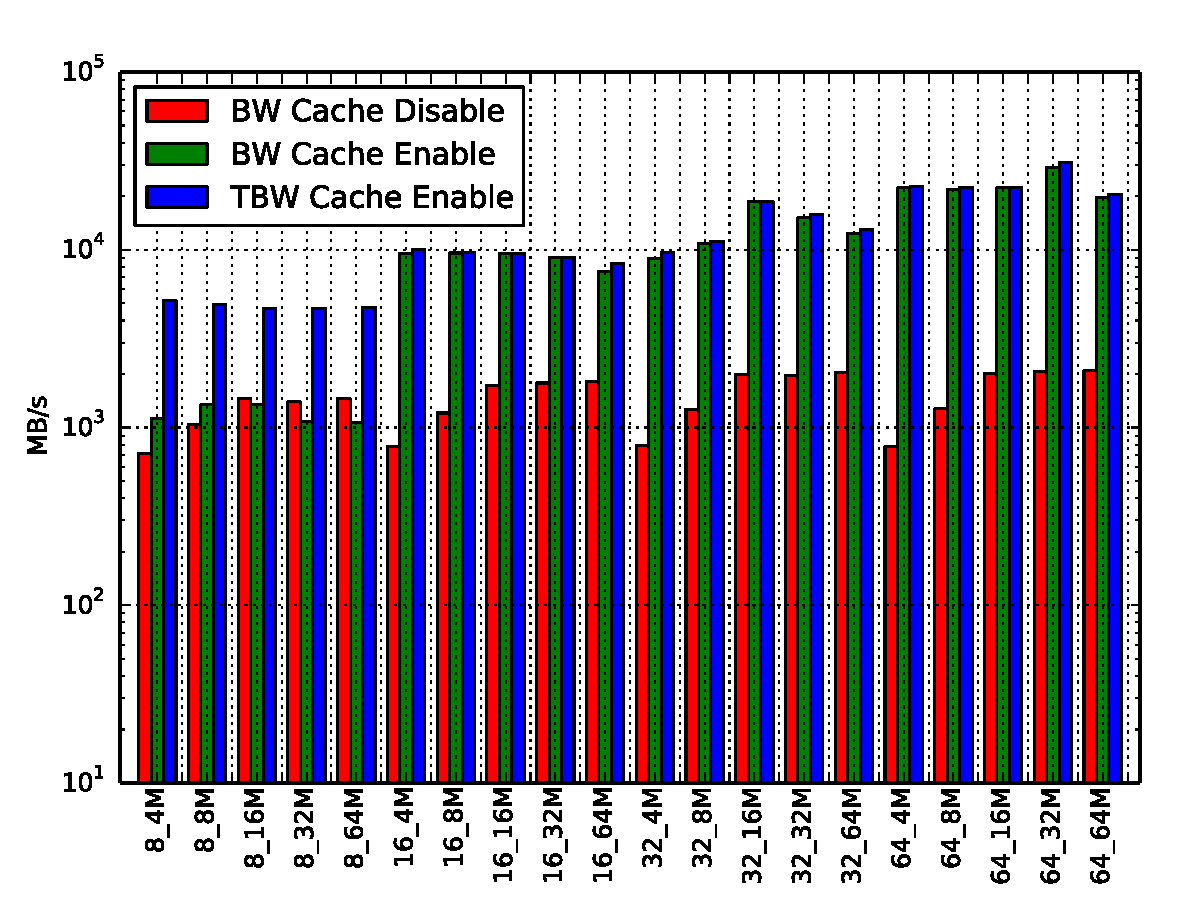
\includegraphics[width=\textwidth]{figures/coll_perf_32GB_30sec_bw}
  \caption{}
  \label{figure: collperf-bw}
  \end{subfigure}
  \begin{subfigure}[]{0.7\textwidth}
  \centering
  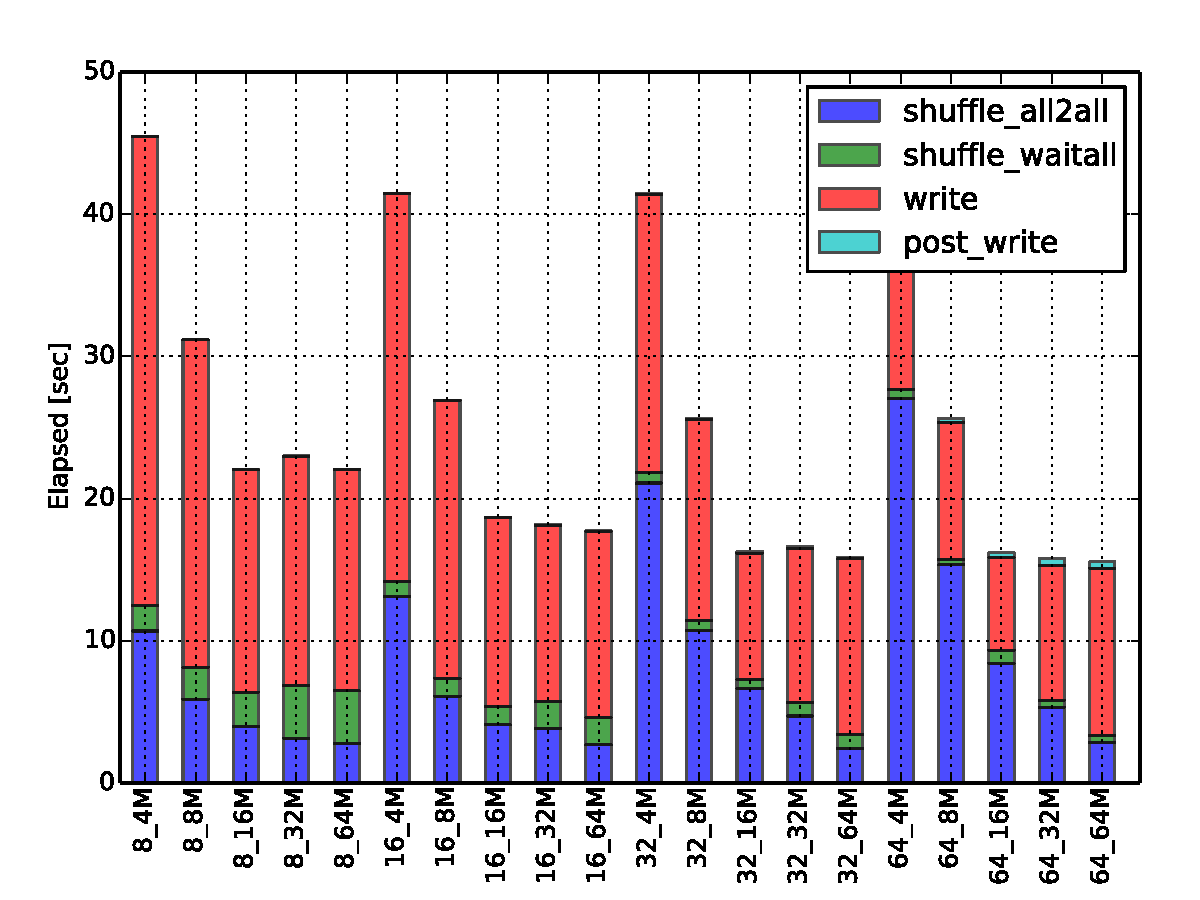
\includegraphics[width=\textwidth]{figures/coll_perf_32GB_30sec_elapsed_disable}
  \caption{}
  \label{figure: collperf-elaps-disable}
  \end{subfigure}
  \begin{subfigure}[]{\textwidth}
  \centering
  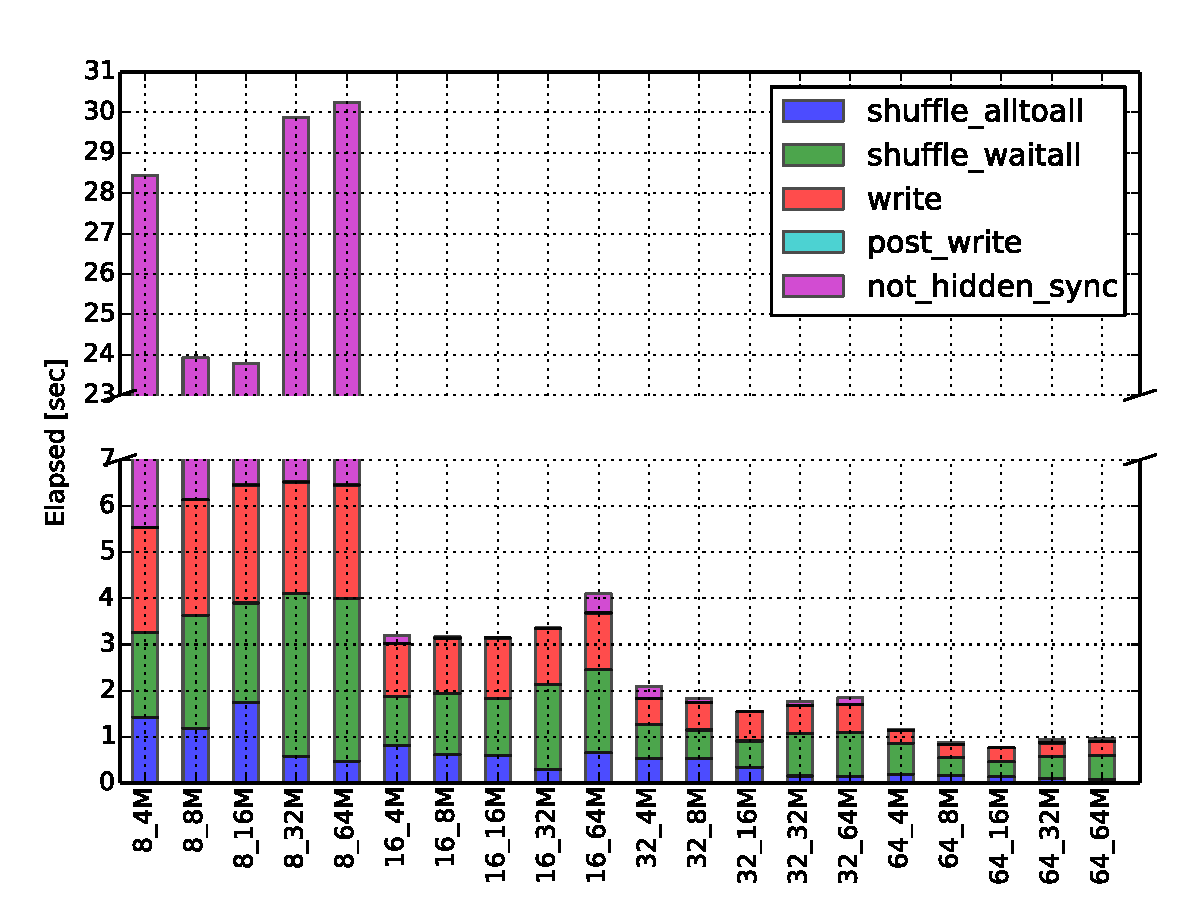
\includegraphics[width=0.7\textwidth]{figures/coll_perf_32GB_30sec_elapsed_enable}
  \caption{}
  \label{figure: collperf-elaps-enable}
  \end{subfigure}
  \caption{Perceived and theoretical write bandwidth for all combinations of aggregators and collective buffer sizes (\ref{figure: collperf-bw}); 
  collective I/O contribution breakdown when cache is disabled (\ref{figure: collperf-elaps-disable}); collective I/O contribution breakdown when cache is 
  enabled (\ref{figure: collperf-elaps-enable}).}
  \label{figure: collperf-results}
\end{figure*}

Figure~\ref{figure: collperf-results} shows the results for the perceived and theoretical write bandwidth (\ref{figure: collperf-bw}), as well as the single 
performance contributions for standard collective I/O (\ref{figure: collperf-elaps-disable}) and cached collective I/O (\ref{figure: collperf-elaps-enable}). 
We start by analyzing the behaviour of standard collective I/O in Figure~\ref{figure: collperf-elaps-disable}.

Let us start by considering the effect of different collective buffer sizes on the collective write time. To this purpose we fix the number of aggregators and look at 
the time contributions when increasing the buffer size from 4~MB to 64~MB. We first observe that the global synchronization cost (\textit{shuffle\_all2all}) decreases.
This is consistent with the ext2ph algorithm behaviour because, as we have already said, increasing the collective buffer size decreases the number of two phase I/O rounds
and therefore the number of global synchronization events (\texttt{MPI\_Alltoall()}). The write cost associated to POSIX write operations also decreases because we are
writing to more I/O servers at the same time (recall that we are using four I/O servers and a stripe size of 4~MB). When the buffer size is 4~MB we only write to one
I/O server, when the buffer size is 16~MB we write to all of them. This also explains why further increasing the buffer size does not reduce the write cost. The
communication cost (\textit{shuffle\_waitall}), on the other hand, increases with the buffer size. This happens because, although the total amount of data shuffled remains
constant, the amount of data shuffled during every round of two phase I/O increases, saturating the aggregators network bandwidth. When we use 8 aggregators, for example, 
up to 32~MB of data are shuffled across the network when using 4~MB buffers, up to 512~MB with 64~MB buffers. Finally, we can look at what happens when we keep the
buffer size constant and increase the number of aggregators. In this case we notice that the global synchronization cost increases. This is due to the increased network 
concurrency at the I/O servers. Finally, \textit{post\_write} time, represented by \texttt{MPI\_Allreduce()}, does not contribute considerably to overall performance because
the corresponding global synchronization event is only encountered once.

We now look at what happens to the ext2ph contributions when we use the cache (Figure~\ref{figure: collperf-elaps-enable}). The global synchronization cost can be still reduced
by increasing the collective buffer size, but because local SSDs are not shared with other nodes across the network, I/O requests can be served in a more predictable way. This
allows aggregators to complete I/O faster and consequently reduces the global synchronization overhead related to collective communications. Write time is not affected visibly
by larger buffers because every aggregator writes data locally. Communication cost is not affected because the communication pattern does not change with respect to the non-cached
collective I/O case. Additionally, we now have a new contribution representing the cache synchronization time that cannot be overlapped with computation (\textit{not\_hidden\_sync}).
We can observe that this contribution is consistent only for 8 aggregators. In fact, when using 8 aggregators the aggregated bandwidth provided by the local SSD
devices cannot match the parallel file system.

The described behaviours are reflected on the perceived write bandwidth shown in Figure~\ref{figure: collperf-bw}. In particular we observe that only the 8 aggregators
configuration achieves worse performance than the standard collective I/O case. All the remaining configurations always achieve better performance and can provide up to
30~GB/s when using 64 aggregators and 32~MB buffer size, an improvement of 15 times. We also observe that the aggregated bandwidth can be scaled by increasing the number 
of aggregators and thus the number of available SSD devices. Finally, when using the cache, the buffer size has limited impact on write bandwidth meaning that we can achieve 
good performance with small buffer sizes, reducing the pressure of collective I/O on system memory.

\subsubsection{Flash-IO}
Flash-IO is the I/O kernel of the Flash application~\cite{Rosner2000}. The Flash-IO benchmark writes three different
files, a checkpoint file a plot file with centered data and a plot file with corner data. The checkpoint file is written using either parallel HDF5 or PnetCDF. We modified the
benchmark to only write the checkpoint file using parallel HDF5. In our configuration, every process in the Flash application writes 80 blocks. Each block contains 16 zones, and 
each zone has 24 variables encoded with 8~bytes, for a total of 768~KBs/block/proc, for a total file size of about 30~GB. Blocks are not written to the checkpoint file with a 
single collective write operation, like in coll\_perf, but instead using multiple collective operations through \texttt{MPI\_File\_write\_at\_all()}. Similarly to coll\_perf we 
have modified the Flash-IO workflow to completely hide the cache synchronization cost.

\begin{figure*}[]
  \centering
  \begin{subfigure}[]{0.7\textwidth}
  \centering
  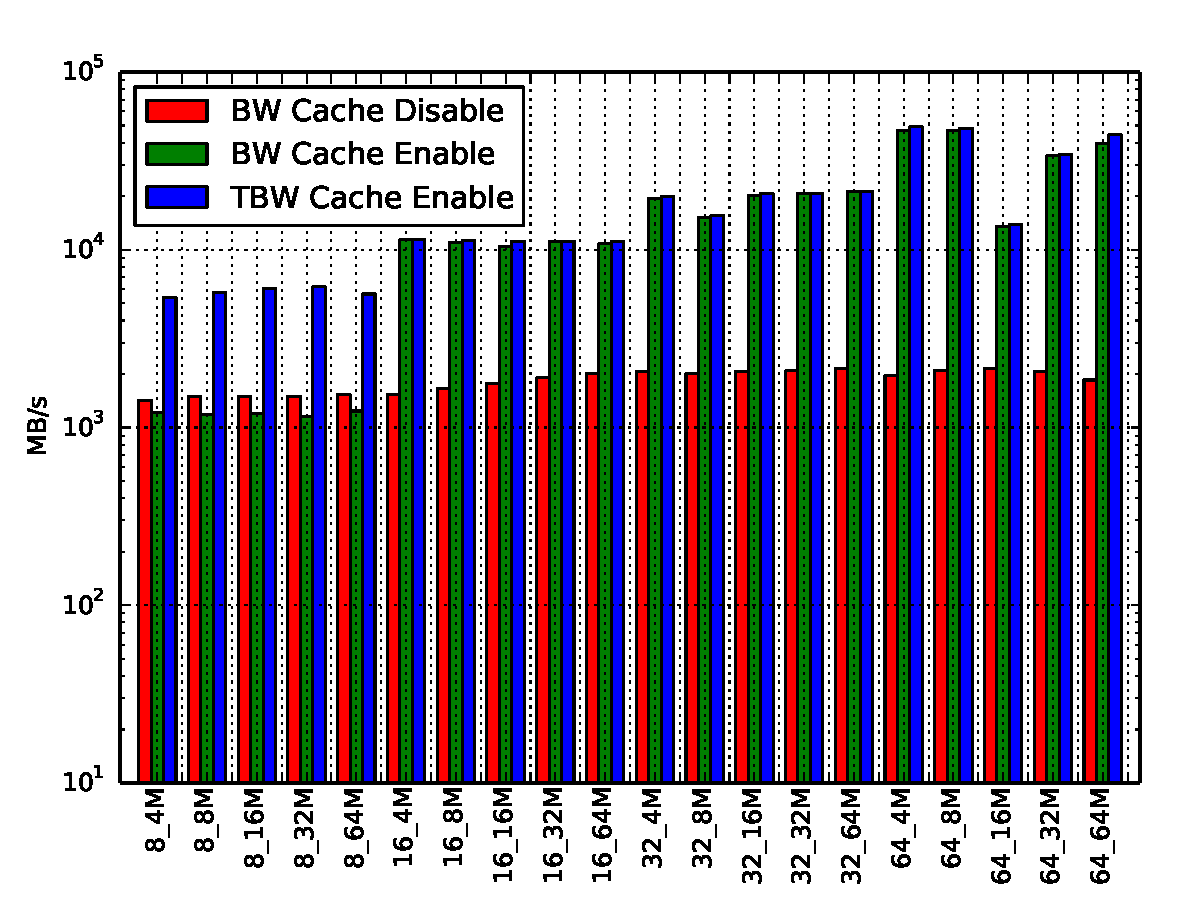
\includegraphics[width=\textwidth]{figures/flash_32GB_30sec_bw}
  \caption{}
  \label{figure: flash-bw}
  \end{subfigure}
  \begin{subfigure}[]{0.7\textwidth}
  \centering
  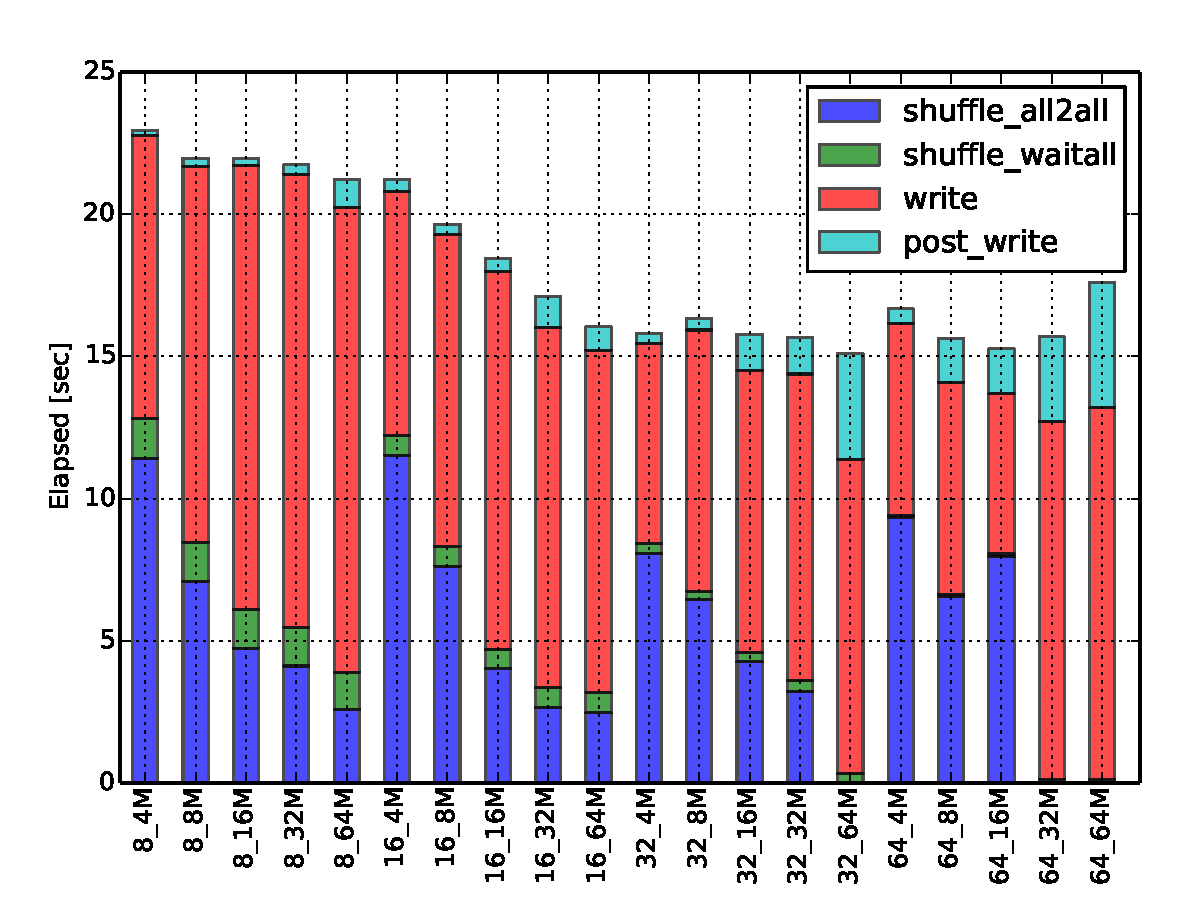
\includegraphics[width=\textwidth]{figures/flash_32GB_30sec_elapsed_disable}
  \caption{}
  \label{figure: flash-elaps-disable}
  \end{subfigure}
  \begin{subfigure}[]{\textwidth}
  \centering
  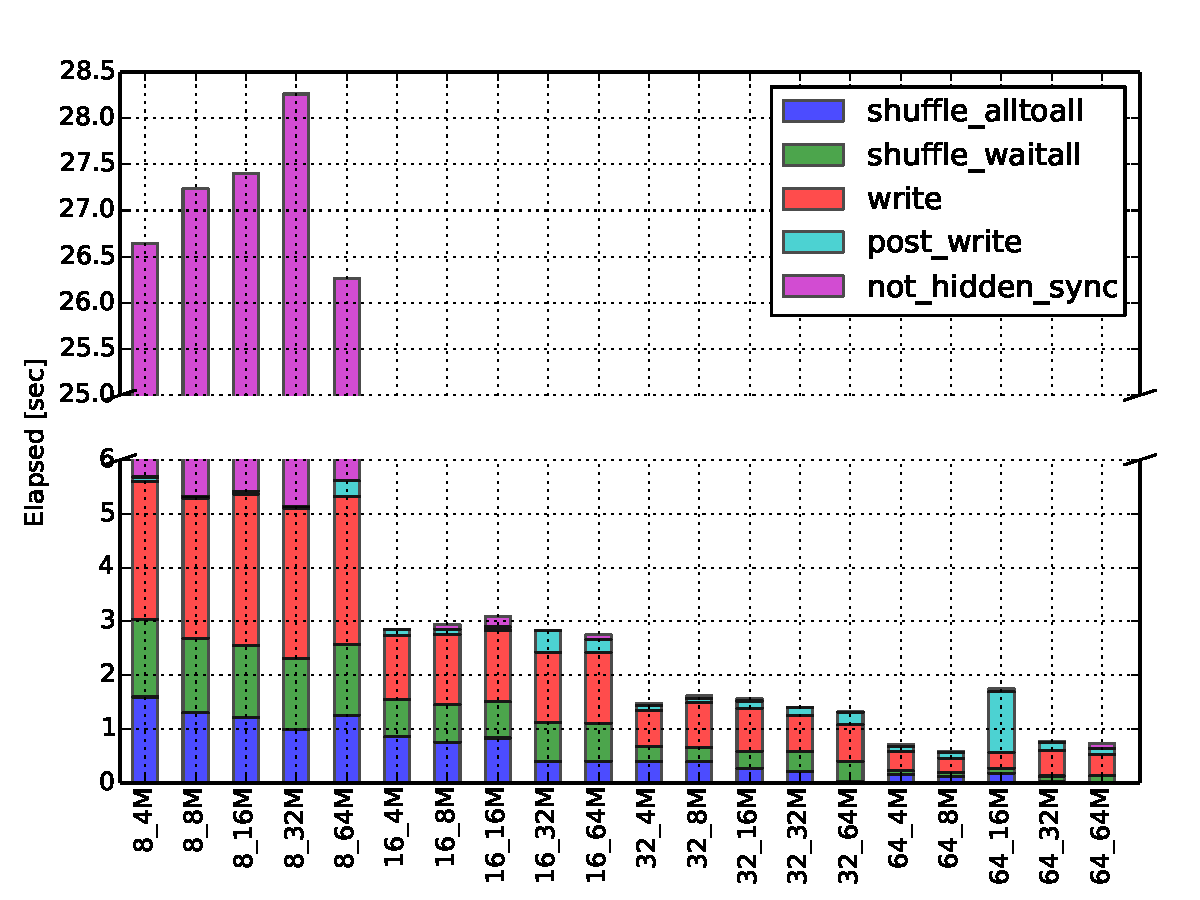
\includegraphics[width=0.7\textwidth]{figures/flash_32GB_30sec_elapsed_enable}
  \caption{}
  \label{figure: flash-elaps-enable}
  \end{subfigure}
  \caption{Perceived I/O bandwidth for all combinations of aggregators and collective buffer sizes (\ref{figure: flash-bw}); collective I/O contribution breakdown 
  when cache is disabled (\ref{figure: flash-elaps-disable}); collective I/O contribution breakdown when cache is enabled (\ref{figure: flash-elaps-enable}).}
  \label{figure: flash-results}
\end{figure*}

Like in coll\_perf, for Flash-IO we measured the same performance parameters varying the number of aggregators and collective buffer size. Results are shown in Figure~\ref{figure:
flash-results}. When the cache is disabled, again we observe reduction of the global synchronization cost for increasing buffer sizes. Communication cost this time does not increase 
with the buffer size. In fact, the file domain size varies from about 49~MB to 6~MB, for 8 and 64 aggregators respectively. This is much less than the amount of data exchanged in 
coll\_perf and thus can be better served by the network infrastructure. Write performance, on the other hand, get worse as the buffer size increases. This behaviour is probably due 
to the fact that, unlike in coll\_perf, writes are not multiple of the stripe size and therefore there might be additional locking overhead at the file system level.
Finally, we observe that the \textit{post\_write} contribution is more consistent this time. The reason, as already anticipated, is that Flash-IO does not write data with a single
collective operation but instead uses multiple operations, thus increasing the number of \texttt{MPI\_Allreduce()} calls at the end of the ext2ph algorithm.

When the cache is enabled we can observe much better performance. Once again, 8 aggregators are not sufficient to completely hide cache synchronization cost to the application. As last
note, we see that in the case of 64 aggregators and 16~MB buffer size there is a drop of write bandwidth in Figure~\ref{figure: flash-bw} due to a peak in the \textit{post\_write}
contribution in Figure~\ref{figure: flash-elaps-enable}. This tells us that when using the cache, although we can minimize the scheduling effects on I/O requests, a small variation 
in the I/O time across aggregators can produce substantial effects on the perceived bandwidth. Indeed, we can see a drop of about 25~GB/s with respect to the 64 aggregators and 
32~MB buffer size.

\begin{figure*}[]
  \centering
  \begin{subfigure}[]{0.7\textwidth}
  \centering
  \includegraphics[width=\textwidth]{figures/ior_32GB_30sec_bw}
  \caption{}
  \label{figure: ior-bw}
  \end{subfigure}
  \begin{subfigure}[]{0.7\textwidth}
  \centering
  \includegraphics[width=\textwidth]{figures/ior_32GB_30sec_disable}
  \caption{}
  \label{figure: ior-elaps-disable}
  \end{subfigure}
  \begin{subfigure}[]{\textwidth}
  \centering
  \includegraphics[width=0.7\textwidth]{figures/ior_32GB_30sec_enable}
  \caption{}
  \label{figure: ior-elaps-enable}
  \end{subfigure}
  \caption{Perceived I/O bandwidth for all combinations of aggregators and collective buffer sizes (\ref{figure: ior-bw}); collective I/O contribution breakdown when cache is 
  disabled (\ref{figure: ior-elaps-disable}); collective I/O contribution breakdown when cache is enabled (\ref{figure: ior-elaps-enable}).}
  \label{figure: ior-results}
\end{figure*}

\subsubsection{IOR}
IOR\footnote{\url{http://www.nersc.gov/users/computational-systems/cori/nersc-8-procurement/trinity-nersc-8-rfp/nersc-8-trinity-benchmarks/ior/}.} is a parallel I/O benchmark that supports 
both independent and collective I/O operations using a variety of interfaces including POSIX-IO, MPI-IO and HDF5. Although IOR supports collective I/O operations it does not allow
users to define strided patterns (like the one in coll\_perf) using file views. Strided layouts can be built by reading or writing multiple data segments. A segment is a contiguous byte 
range in the file accessed by only one process. For example, if we have four processes and each of them writes three segments of 64~MB, the first process writes its first segment
starting at 0~MB and ending at 64~MB, the second process writes its first segment starting at 64~MB and ending at 128~MB, and so on.
When all the processes have written the first segment they initiate another write operation for the second segment starting at offset 256~MB. Every segment is written with an independent
collective write operation.

In our experiments we used 8 segments and each of the 512 processes writes 8~MB for segment, for a total of 32~GB file. Unlike the previous two cases, in IOR we follow the workflow
depicted in Figure~\ref{figure: workflow}; meaning that for the last write phase cache synchronization will not be hidden by any following compute phase. This allows us to show what 
a real world use case would look like.

Figure~\ref{figure: ior-results} shows the obtained results. These results are similar to the previous except for the fact that now the \textit{not\_hidden\_sync} contribution is
visible for every collective I/O configuration. The cache synchronization cost represents a huge part of the total I/O time. Although, absolute bandwidth performance are lower 
than previous results we still have that writing data to local SSD devices can give advantages over the baseline ext2ph strategy. In fact, on average we can at least triple the 
perceived write bandwidth going from about 2~GB/s to 6~GB/s.

The reduction of the cache synchronization cost has not been explored in our work and therefore leaves opening for future optimizations that will be discussed in the conclusion
chapter.

\subsection{Conclusions}
In this section we have analyzed collective write performance using a range of different benchmarks that use both synthetic and real I/O patterns to transfer large checkpoint buffers
to the parallel file system. Our tests show how collective I/O is mainly limited by the ext2ph algorithm global synchronization overhead and how the use of fast local non-volatile
memories is effective in reducing the impact that global file system latency has on such synchronization by taking it out of the critical I/O path. Our work practically proves
how next generation I/O systems can benefits from multi tier storage and how first tier non-volatile storage devices can be leveraged by giving the user more control over them.

%!TEX root = ../main.tex
\section{Conclusion \& Future Work}
\label{sec: mercury_conclusion}

In this chapter we presented a guided I/O framework prototype that can be used to set POSIX advice and GPFS hints on behalf of applications transparently to the user. This is done by adding annotations regarding which regions of a file to prefetch into a configuration file that is afterwards fed to the \textit{Assisted I/O library} and \textit{Advice Manager} modules. %We demonstrated that using our prototype the non-optimal I/O pattern of a real application can be adapted to the underlying storage system to improve performance. %This is useful for all those applications that access their data using an immutable I/O pattern, like the `ROOT' application here presented.

%We focused predominantly on read patterns which characterize a class of scientific applications known as big data science analytics. These class of applications differ from HPC applications in the type of I/O pattern they use. Indeed, HPC applications are dominated by writing of large amounts of checkpoint data to a shared (N-1 pattern) or multiple files (N-N pattern) for restart purposes or, more generally, for post processing. Big data analytics applications, on the other hand, read large amounts of input data for processing and write very little volumes of output data (results) to the file system. Currently, there is a convergence of these two paradigms that brings big data analytics applications to run on high-end computing clusters, typically as post processing phase for data generated by HPC applications such as, e.g., climate and earthquake simulations. Here we considered `ROOT' as representative for big data science analytics and we demonstrated that by using the hints API provided by the file system in an appropriate way it is possible to improve the storage system usage and ultimately the application performance.  
 
In the future we plan to further explore the problem of data science analytics applications in HPC, studying more profusely the different types of existing I/O patterns and how hints can be used to improve the cache utilization efficiency and thus applications' performance. Moreover, although not explicitly treated here, we recognise how important is to automatically extract information concerning the application's I/O pattern profile. Almost all the current analysis tools, including the ones we have used, approach the I/O pattern analysis problem from an ultra fine-grain point of view (i.e. considering the offset and length requests) with the result of having a very specific file per application characterization. On the other hand, in this work we have observed that a course-grain approach (i.e. considering blocks instead of single requests) can be more beneficial when trying to extract the general application behaviour. The study of an automatic I/O pattern analysis tool with the described features will be thus part of future work. 
%In the future we plan to extend the \textit{Advice Manager} to provide support for MPI I/O hints that currently have to be hard coded into the application. In this way administrators could use our mechanism to change, for instance, the striping policy of a specific file to adapt it to the underlying storage system configuration, without modifying the application. The integration of cluster aware I/O support will also compensate for the lack of file access global scope in the current version. 

%TODO: consider a comment about how this won't work as a cluster-aware installation - open files are not shared between nodes, they have an independent view. 

%TODO: a criticism may be that 'we never run the application with the same data', and 'changing the data changes the applications behaviour', so the learning approach isn't valid. A sentence or two to explain that while the data may change, the manner in which the program accesses it does not. A good example of this is a climate simulator.

\cleardoublepage

%*******************************************************************************************
% END OF CHAPTERS
%*******************************************************************************************

%*******************************************************************************************
% BIBLIOGRAPHY
%*******************************************************************************************
\cleardoublepage
\addcontentsline{toc}{chapter}{Bibliography}

\bibliographystyle{alpha}
\bibliography{bibliography}

%*******************************************************************************************
% LIST OF FIGURES
%*******************************************************************************************
\listoffigures
\cleardoublepage

%*******************************************************************************************
% LIST OF TABLES
%*******************************************************************************************
\listoftables
\cleardoublepage

%*******************************************************************************************
%END BIBLIOGRAFIA
%*******************************************************************************************
\end{document}
%*******************************************************************************************
%*******************************************************************************************
%  END   DOCUMENT 
%*******************************************************************************************
%*******************************************************************************************
